%======================================================================
%  CSE 450 Capstone Project -- Report
%  Department of Computer Science and Engineering, BUET
%
%  1. Fill in the block below.
%  2. Write each chapter in chapters/*.tex, replacing every gray italic
%     \guidance{...} note with your content.
%  3. Add more chapters to best present your work, if needed.
%  4. Build:  latexmk -pdf template.tex   (or Overleaf, compiler: pdfLaTeX)
%======================================================================
\documentclass[12pt,a4paper,oneside]{report}
\usepackage{cse-capstone}
\usepackage{longtable}
\usepackage{array}
\usepackage{booktabs}
\usepackage{tikz}
\usetikzlibrary{calc}
\usetikzlibrary{arrows.meta, positioning, fit, backgrounds}

% ---------------------------------------------------------------------
\newcommand{\ProjectTitle}{Project Intelligence Platform for Software Quality and Performance Tracking}
\newcommand{\Session}{Session 2024--2025}
\newcommand{\SubmissionDate}{Sep 2026}
\newcommand{\Supervisors}{%
  Mohammad Sadat Hossain\\
  Lecturer, Department of CSE, BUET}
% Team members are listed in frontmatter/titlepage.tex and declaration.tex
% ---------------------------------------------------------------------

\hypersetup{pdftitle={\ProjectTitle}}

\begin{document}

\pagenumbering{gobble}
\thispagestyle{empty}
\begin{center}

{\large CSE450 Capstone Project Report}

\vspace*{\stretch{2}}
{\LARGE\bfseries \ProjectTitle}

\vspace*{\stretch{4}}
{\large Submitted by}\\[10pt]
\begin{tabular}{ll}
  Afham Adian & 2105119 \\
  Abdullah Al Mahmud & 2105120 \\
  Arafat Rahman & 2105118 \\
  Tahmidul Islam Omi & 2105115 \\
  Arnab Sarker & 2105099
\end{tabular}

\vspace*{\stretch{3}}
{\large Supervised by}\\[10pt]
\Supervisors

\vspace*{\stretch{3}}
\includegraphics[width=30mm]{buet_logo.png}\\[8pt]
\textbf{Department of Computer Science and Engineering}\\
{\large\bfseries Bangladesh University of Engineering and Technology}\\
Dhaka, Bangladesh

\vspace*{\stretch{1}}
\Session\\
\SubmissionDate

\end{center}
\clearpage

\pagenumbering{roman}
\begin{center}
  {\Large\bfseries CANDIDATES' DECLARATION}
\end{center}
\addcontentsline{toc}{chapter}{Candidates' Declaration}

\vspace{20pt}
We declare that the work presented in this report, titled
``\ProjectTitle'', is the outcome of the engineering work carried out by us
under the supervision named on the title page.

All prior work, third-party code, libraries, data, copyrighted material, and
tools used in the project have been properly acknowledged. Any use of
generative AI tools has been disclosed. We accept accountability and
responsibility for the accuracy and integrity of this report and for our
individual contributions to the project.

\vspace{15mm}
\begin{tabular}{>{\raggedright\arraybackslash}p{0.45\textwidth} >{\raggedright\arraybackslash}p{0.45\textwidth}}
  \rule{0.4\textwidth}{0.4pt} & \rule{0.4\textwidth}{0.4pt} \\
  Afham Adian (2105119) & Abdullah Al Mahmud (2105120) \\[15mm]
  \rule{0.4\textwidth}{0.4pt} & \rule{0.4\textwidth}{0.4pt} \\
  Arafat Rahman (2105118) & Tahmidul Islam Omi (2105115) \\[15mm]
  \rule{0.4\textwidth}{0.4pt} & \\
  Arnab Sarker (2105099) &
\end{tabular}
\clearpage

\chapter*{ACKNOWLEDGEMENT}
\addcontentsline{toc}{chapter}{Acknowledgement}

From the bottom of our hearts, we thank our supervisor, \textbf{Mohammad Sadat
Hossain}, Lecturer, Department of Computer Science and Engineering, BUET, whose
guidance, patience and steady encouragement carried this project through the semesters. Our supervisor helped us turn a broad problem into a focused piece of
engineering, questioned our assumptions when they needed questioning, and kept
us moving forward when progress was slow. This work would not have taken its
present shape without that support.

We are equally and deeply grateful to the \textbf{Chief Technical Officer of
Spectrum Software \& Consulting Pvt.\ Ltd.\ (SSCL)}, who brought us the problem
this project set out to solve and generously gave time throughout development.
Each major stage of the system was reviewed with SSCL's CTO, and that candid
direction shaped Pulse's audience, its commitment to anonymous surveys, how and
how often surveys reach developers, and the adoption of the action log. This
industry perspective gave the project a purpose beyond the classroom, and we
offer our sincere thanks for the trust and support we received.
\clearpage

\chapter*{ABSTRACT}
\addcontentsline{toc}{chapter}{Abstract}

Software organisations run each project through separate tools for version
control, issue tracking, static code analysis and CI/CD, and each tool reports
its own metrics on its own scale. Judging whether a project is healthy therefore
means reconciling four or five dashboards by hand. At Spectrum Software \&
Consulting Pvt.\ Ltd.\ (SSCL), the industry partner that raised the problem,
this is done rarely. Projects cannot be compared like for like, and a slowly
deteriorating project is noticed only once deadlines slip. The tools also
capture nothing about how the team is faring, or about what management did in
response and whether it helped.

This project designed and built \emph{Pulse}, a multi-tenant engineering-health
platform. Scheduled and on-demand synchronisation pulls metrics through a
connector abstraction into immutable snapshots. A deterministic rule-based model
converts them into seven health scores and an overall score on a common 0--100
scale. An absent metric is excluded and the remaining weights are renormalised,
and every score decomposes into the signals, weights and contributions that
produced it. AI-generated surveys, delivered by email, collect team feedback
without storing any respondent identity. An action log records management
interventions and prompts a later review of their effectiveness. The system is
built with TypeScript, PostgreSQL, Redis and React. It is deployed on free-tier
services at no monetary cost.

Verification combined 142 automated tests enforced as a required CI check,
inspection, end-to-end demonstration on the team's own repositories, and four
targeted investigations. The system was also reviewed with SSCL's Chief
Technical Officer in five meetings. Of 41 functional requirements, 38 are met;
of 26 non-functional requirements, 21 are met. The investigations showed that
renormalisation stops a project being penalised for an unconnected tool (a
score of 80 rather than 12 in a worked example). They also found that no stored
record links a survey response to its author. Six connectors across the four
tool categories were delivered, two more than planned. The main limitations are
that AI-assisted action search does not fall back automatically when its
provider is unavailable, and that the rate-limit capacity per shared credential
is unquantified. Overall test coverage is also low, with no frontend tests.

\vspace{12pt}
\noindent\textbf{Keywords:} software project health; engineering metrics;
explainable scoring; anonymous surveys; tool integration
\clearpage

\tableofcontents
\listoffigures
\listoftables

\clearpage
\pagenumbering{arabic}
% Chapter 1 -- Rubric: PO1 (1.1), PO2 (problem identification), PO3 (3.2 objectives)
\chapter{Problem Identification and Formulation}
\label{ch:problem}

\section{Background and Motivation}
\label{sec:background}

A software organisation runs each of its projects through several specialised
tools: a version-control platform for source code and code review, an
issue-tracking platform for planning and sprint management, a static
code-analysis service for code quality, and a CI/CD service for builds and
deployments. Each tool exposes its own dashboard, reports its own metrics in its
own vocabulary, and answers questions only about its own slice of the work.
None of them answers the question that engineering leadership actually asks:
\emph{is this project, taken as a whole, healthy, and is it improving or
deteriorating?}

The consequence, as described by Spectrum Software \& Consulting Pvt.\ Ltd.\
(SSCL), the industry partner that originated this project, is that assessing the state of a single project means opening
four to five dashboards in turn and reconciling their readings by judgement.
Doing this across a whole portfolio is impractical, so it is done
infrequently. As a result, a project that is gradually deteriorating is often
noticed only after the damage has become visible as missed deadlines or failing
builds.

Two further gaps compound this. First, tool metrics describe what the code and
the pipeline are doing, but not how the team is doing; low morale, persistent
blockers, and loss of confidence in a plan are often the earliest signals of a
project in trouble, and they appear in no dashboard. Second, when a manager does
identify a problem and acts on it, the action is recorded nowhere, so there is
no later way to tell whether the intervention worked.

Pulse addresses these gaps. It ingests metrics from the separate tools,
normalises them into comparable health scores on a single scale, keeps every
score explainable in terms of the metrics that produced it, collects anonymous
team feedback that metrics cannot capture, and records the management actions
taken in response so that their effectiveness can be reviewed. It is designed as
a trend indicator, revealing how projects move over weeks and months, rather
than as a real-time monitor.

\section{Problem Statement}
\label{sec:problem-statement}

Engineering leadership and project managers at software organisations such as
SSCL oversee many projects at once, and each project produces its data in
several independent tools: version control, issue tracking, static code
analysis and CI/CD. Every tool reports its own metrics on its own scale, and
none of them offers a common notion of whether a project is healthy. To judge a
project's condition, a manager has to gather readings from each tool separately
and reconcile them by hand, and the tools capture nothing about how the team
itself is faring or about what management did when a problem was found.

Because this reconciliation is slow and manual, it is done infrequently and
inconsistently; projects cannot be compared on a like-for-like basis; and a
project that is gradually deteriorating is usually recognised only once the
damage has become visible. The early warning signs that only the team is aware of, such
as people losing motivation or work that keeps getting stuck, never reach any
dashboard, and because
interventions are not recorded, whether they helped is never known. What is
missing is a single, comparable and explainable view of project health that
draws on all of these tools, that captures the team's own signal without
exposing individuals, and that connects management action to measured outcome.
Closing that gap is the problem this project addresses.

\section{Complexity of the Problem}
\label{sec:complexity}

\begin{longtable}{
  >{\raggedright\arraybackslash}p{0.05\textwidth}
  >{\raggedright\arraybackslash}p{0.38\textwidth}
  >{\raggedright\arraybackslash}p{0.45\textwidth}
}
\caption{Complex engineering problem characteristics (P1--P7) and evidence from this project}
\label{tab:complexity}\\
\toprule
\textbf{Code} & \textbf{Definition} & \textbf{Evidence from this project} \\
\midrule
\endfirsthead
\toprule
\textbf{Code} & \textbf{Definition} & \textbf{Evidence from this project} \\
\midrule
\endhead
\bottomrule
\endlastfoot
P1 & \textbf{Depth of knowledge required.} Cannot be resolved without in-depth engineering knowledge at the level of one or more of K3, K4, K5, K6, or K8, which allows a fundamentals-based, first-principles analytical approach. &
K3: the weighted-normalisation scoring model, its handling of missing inputs, and its exact decomposition into per-metric contributions.
K4 and K6: asynchronous job processing with retries and idempotent scheduling; rate-limit-aware integration with third-party REST and GraphQL APIs; credential encryption, password hashing and session security.
K5: the connector abstraction that isolates provider-specific ingestion from scoring, and the snapshot-based data model that makes every score reproducible. \\
\addlinespace
P2 & \textbf{Range of conflicting requirements.} Involves wide-ranging or conflicting technical, engineering, and other issues. &
\guidance{To be completed after discussion with the team} \\
\addlinespace
P3 & \textbf{Depth of analysis required.} Has no obvious solution and requires abstract thinking and originality in analysis to formulate suitable models. &
There is no established mapping from heterogeneous tool metrics to a single comparable scale. The team had to derive, per metric, a normalisation function and weight, define how absent metrics are treated, and design the scores so that they remain exactly explainable; and had to design survey aggregation that yields team-level insight without any per-respondent record. \\
\addlinespace
P4 & \textbf{Familiarity of issues.} Involves infrequently encountered issues. &
\guidance{To be completed after discussion with the team} \\
\addlinespace
P6 & \textbf{Extent of stakeholder involvement and conflicting requirements.} Involves diverse groups of stakeholders with widely varying needs. &
Seven stakeholder groups (\Cref{tab:stakeholders}): the client's leadership, its managers, its developers as data subjects, the tenant administrator, the academic supervisor, external service providers as constraint setters, and the development team, whose needs conflict as set out under P2. \\
\addlinespace
P7 & \textbf{Interdependence.} Is a high-level problem including many component parts or sub-problems. &
Authentication and tenancy; workspace and connector configuration; metric ingestion and scheduling; scoring; survey generation, distribution and analysis; and the action log. These are dependent: scoring requires ingestion, survey generation is driven by scores and their trends, actions are recorded against both, and scheduling must space projects that share a credential to stay within rate limits. \\
\end{longtable}

\begin{longtable}{
  >{\raggedright\arraybackslash}p{0.08\textwidth}
  >{\raggedright\arraybackslash}p{0.80\textwidth}
}
\caption{Knowledge profiles referenced by P1}
\label{tab:knowledge-profile}\\
\toprule
\textbf{Code} & \textbf{Description} \\
\midrule
\endfirsthead
\toprule
\textbf{Code} & \textbf{Description} \\
\midrule
\endhead
\bottomrule
\endlastfoot
K3 & A systematic, theory-based formulation of engineering fundamentals required in the engineering discipline. \\
\addlinespace
K4 & Engineering specialist knowledge that provides theoretical frameworks and bodies of knowledge for the accepted practice areas in the engineering discipline; much is at the forefront of the discipline. \\
\addlinespace
K5 & Knowledge that supports engineering design in a practice area. \\
\addlinespace
K6 & Knowledge of engineering practice (technology) in the practice areas in the engineering discipline. \\
\addlinespace
K8 & Engagement with selected knowledge in the research literature of the discipline. \\
\end{longtable}

\section{Project Objectives and Scope}
\label{sec:objectives}

The project set out to achieve the following objectives:

\begin{enumerate}
  \item \textbf{Consolidate} the metrics of a project's version-control,
  issue-tracking, code-analysis and CI/CD tools into a single dashboard, so
  that routine status assessment needs none of the tools' own dashboards.
  \item \textbf{Normalise} those heterogeneous metrics into seven health scores
  on a common 0--100 scale, plus an overall score, so that any two projects
  can be compared directly.
  \item \textbf{Explain} every score on request: which metrics produced it,
  their measured values, their weights, and each one's contribution.
  \item \textbf{Capture} qualitative team feedback through anonymous surveys,
  with no stored link between a respondent and their answers.
  \item \textbf{Record} the management actions taken in response to identified
  problems, and prompt for a review of their effectiveness after a set
  interval.
  \item \textbf{Accumulate} health history automatically on a fixed schedule,
  so that trends build up without anyone triggering a synchronisation.
  \item \textbf{Remain extensible}, so that a further tool provider can be
  added without changing the scoring logic.
\end{enumerate}

\textbf{Scope.} The following is within the scope of the project:

\begin{itemize}
  \item One connector for each tool category: GitHub (version control), Jira
  (issue tracking), SonarCloud (code quality) and GitHub Actions (CI/CD).
  \item Multi-tenant organisations with administrator and member roles;
  workspaces bound to a version-control organisation and access token; import
  of repositories as projects.
  \item On-demand and scheduled synchronisation, an immutable snapshot
  history, and portfolio and per-project dashboards with trends and score
  breakdowns.
  \item Automatically generated, editable survey questions; one scheduled
  survey per project per month plus on-demand surveys; anonymous responses;
  and survey analysis.
  \item A management action log with keyword and semantic search and
  effectiveness review.
  \item Email delivery of verification codes, password resets, invitations and
  surveys, and broadcast of survey links to Slack and Discord.
\end{itemize}

The following is explicitly outside the scope:

\begin{itemize}
  \item Real-time monitoring; the system is a trend indicator operating on a
  scheduled cadence.
  \item Version-control providers other than GitHub and CI/CD systems other
  than GitHub Actions; the connector abstraction allows them, but they were
  not implemented.
  \item Any per-individual performance measurement, ranking or surveillance of
  developers.
\end{itemize}

% Chapter 2 -- Rubric: PO1 (1.1), PO2 (research literature), feeds PO3 and PO11
\chapter{Preliminary Research}
\label{ch:research}

\section{Literature Review}
\label{sec:literature}
A formal literature review is not applicable to this project, which is an
applied engineering effort rather than a research contribution.

\section{Existing Solutions and Technologies}
\label{sec:related}
SSCL, like most software organisations, already relies on a set of
specialised tools that each cover one part of this problem: GitHub for
version control, Jira for issue tracking, SonarQube for static code
analysis, and GitHub Actions for CI/CD. Each is capable and widely adopted,
but each is scoped to its own concern and reports through its own dashboard;
none aggregates across the others, which is exactly the gap described in
Chapter 1.

A category of commercial ``engineering intelligence'' platforms --
LinearB, Swarmia, Faros AI, and Jellyfish among them -- does aggregate
metrics across the delivery pipeline, mostly throughput and cycle-time
figures pulled from version control and issue tracking. They integrate with
the same tools SSCL already uses and produce cross-tool dashboards. However,
they focus almost entirely on delivery velocity and code metrics: none
incorporates the team's own qualitative signal through anonymous surveys,
none records management actions taken in response to a decline or tracks
whether they worked, and all are priced per seat. Static-analysis and CI
dashboards (SonarCloud, GitHub Actions) remain confined to their own tool
with no cross-tool scoring at all.

The gap is a single, explainable health score spanning all four tool
categories, combined with anonymous team feedback and a record of
management action and its effectiveness.

\section{Market and User Research}
\label{sec:market}
The primary users are engineering leaders and project managers at software
organisations that run multiple concurrent projects across a mix of
specialised tools -- version control, issue tracking, static analysis, and
CI/CD -- for each one. SSCL, the project's industry partner, is
representative of this user base and was the direct source of evidence for
the need: its engineering leadership described project-health assessment as
a routine but repetitive task of opening several dashboards on a fixed
cadence and reconciling them by judgement, with no tool available to
aggregate them and no channel through which a team's own sense of how a
project was going ever reached management.

Because SSCL was the only source of user evidence available to the team, no
formal market sizing was attempted. The underlying situation, however, is not
specific to SSCL: any organisation running comparable multi-tool,
multi-project engineering operations faces the same fragmentation, which
suggests demand extends beyond the immediate industry partner.

\section{Feasibility Study}
\label{sec:feasibility}
\textbf{Technical.} GitHub, Jira, SonarCloud and GitHub Actions each expose
documented REST or GraphQL APIs with free-tier rate limits sufficient for a
handful of pilot projects, so all the data the scoring model needs was
obtainable without purchasing access. The team's existing experience with
Node.js, TypeScript, Supabase Postgres and Redis/BullMQ meant the pipeline
could be built on a stack already familiar to it. The main technical risk,
rate limits shared across projects on the same credential, was manageable by
spacing scheduled syncs. Free hosting tiers covered the API and frontend; the
one exception is the background worker, which must run continuously rather
than on demand and currently has no equivalent free serverless option, so it
remains unhosted.

\textbf{Economic.} The system was built entirely on free tiers -- Supabase,
Vercel, Upstash Redis, and the free quotas of the integrated tools -- so
development introduced no cost beyond the team's time. For SSCL, the
expected benefit is reducing the recurring manual effort of dashboard
reconciliation across its portfolio, which comes at no licensing cost to
adopt.

\textbf{Operational.} Adoption only requires the access tokens SSCL already
holds for GitHub, Jira and SonarCloud and a short one-time setup per
project; the underlying tools continue to be used exactly as before, so
operational disruption is minimal.

\textbf{Legal and regulatory.} Access tokens are stored encrypted, and
survey responses are collected with no stored link to a respondent, so no
personally identifiable data is introduced beyond ordinary account
information.

The project was judged feasible on the assumption that SSCL continues to
provide the access tokens and project structure it already uses; the
completed build, delivered within the team's two-semester timeline, confirms
that assessment.

% Chapter 3 -- Rubric: PO2 (2.1), PO3 (3.1, 3.2)
\chapter{Requirements Analysis}
\label{ch:requirements}

\section{Project Objectives and Constraints}
\label{sec:requirements}
% \guidance{Identify all stakeholders (users, client or industry partner,
% administrators, regulators) and their expectations, including conflicting
% ones. Then clearly state the objectives, the functional and non-functional
% requirements, and the constraints (time, budget, platform, data,
% deployment), taking those expectations into account.}

\subsection{Problem Context and Origin}
\label{subsec:problem-context}

The project originated with Spectrum Software \& Consulting Pvt. Ltd. (SSCL), a software development organisation. Engineering leadership at
SSCL monitored the health of their software projects through four to five
separate tool dashboards such as a version control platform (e.g., Github), an issue-tracking and sprint-planning platform (e.g., Jira), a static code-analysis service (e.g., SonarQube), and a CI/CD service (e.g., Jenkins). Each dashboard presented its own metrics in its
own vocabulary, with no shared notion of whether a project was, overall, in good
or poor health. Assessing the state of a single project required visiting every
dashboard in turn and mentally reconciling the results; assessing a portfolio of
projects this way was impractical.

SSCL proposed a platform that would ingest data from these separate tools,
translate heterogeneous raw metrics into a common, comparable scale, and present
the result in a single view. The system described in this report addresses that
problem. It is explicitly positioned as a trend indicator system rather
than a real-time monitoring tool. Its purpose is to reveal how projects and teams
are trending over weeks and months, not to report the state of a build in the
last five minutes.

\subsection{Requirements Elicitation}
\label{subsec:elicitation}

Requirements were gathered through three complementary channels. The primary
channel was a series of meetings with the Chief Technical Officer of
SSCL, who originated the concept and articulated the operational pain point,
the tools in use, and the decisions the system was intended to support. A
secondary channel was an intern at SSCL with prior exposure to the concept,
who provided practical grounding on how the organisation's teams actually work
day to day. The third channel was the team's own analysis such as study of the public
APIs exposed by the candidate tools to establish which metrics were obtainable in
practice, and derivation of a scoring model from that feasible metric set.
Throughout, the university supervisor provided guidance on scope, methodology and
academic rigour.

\subsection{Stakeholders and Their Expectations}
\label{subsec:stakeholders}

\begin{longtable}{
  >{\raggedright\arraybackslash}p{0.08\textwidth}
  >{\raggedright\arraybackslash}p{0.19\textwidth}
  >{\raggedright\arraybackslash}p{0.17\textwidth}
  >{\raggedright\arraybackslash}p{0.40\textwidth}
}
\caption{Stakeholders and their principal expectations}
\label{tab:stakeholders}\\
\toprule
\textbf{ID} & \textbf{Stakeholder} & \textbf{Role} & \textbf{Principal expectations} 
\\
\midrule                                                                             
\endfirsthead
\toprule                                                                             
\textbf{ID} & \textbf{Stakeholder} & \textbf{Role} & \textbf{Principal expectations} \\
\midrule
\endhead
\bottomrule
\endlastfoot
SH-01 & SSCL leadership & Client; originator; primary requirement source
& A single consolidated view replacing four to five dashboards; comparable scores
across projects; early visibility of declining projects \\
\addlinespace
SH-02 & Engineering managers and project managers & Primary end users & Status at a glance; the ability to drill into a score that looks wrong; low operational overhead \\
\addlinespace
SH-03 & Developers employed by SSCL & Data subjects and survey respondents & Assurance that the system is not an instrument of individual surveillance or ranking; minimal interruption; the ability to answer candidly without attribution \\
\addlinespace
SH-04 & Company administrator & Tenant and credential owner & Control over access tokens, workspace membership and tool configuration; assurance that credentials are not exposed \\
\addlinespace
SH-05 & University supervisor & Academic oversight & Methodological rigour, documented decision-making, demonstrable evaluation \\
\addlinespace
SH-06 & External tool and service providers & Constraint setters & Adherence to their authentication models, rate limits, free-tier quotas and terms of service \\
\addlinespace
SH-07 & Development team & Implementers & A scope deliverable by five students within two semesters\\
\end{longtable}

\subsection{Conflicting Expectations and Their Resolution}
\label{subsec:conflicts}

Several stakeholder expectations are in genuine tension. Each conflict was
resolved by an explicit requirement rather than left to implementation judgement.

\begin{longtable}{
  >{\raggedright\arraybackslash}p{0.04\textwidth}
  >{\raggedright\arraybackslash}p{0.34\textwidth}
  >{\raggedright\arraybackslash}p{0.34\textwidth}
  >{\raggedright\arraybackslash}p{0.13\textwidth}
}
\caption{Conflicting stakeholder expectations and their resolution}
\label{tab:conflicts}\\
\toprule
\textbf{\#} & \textbf{Conflict} & \textbf{Resolution} & \textbf{Encoded by} \\
\midrule
\endfirsthead
\toprule
\textbf{\#} & \textbf{Conflict} & \textbf{Resolution} & \textbf{Encoded by} \\
\midrule
\endhead
\bottomrule
\endlastfoot
1 & SH-01 seeks insight into how teams are performing; SH-03, the same
organisation's employees, require that the system not attribute opinions to
individuals & Qualitative feedback is collected anonymously, with no stored link
between a respondent and their answers, and aggregate insight is withheld below a
minimum response count & NFR-07, NFR-08 \\
\addlinespace
2 & SH-01 and SH-02 would benefit from frequent team feedback; SH-03 experience
repeated surveys as interruption and survey fatigue & Survey frequency is capped per
project per month, and a cooldown is enforced per developer across all projects, with
fair rotation for developers on several projects & FR-33, FR-31 \\
\addlinespace
3 & SH-01 expects current data; SH-06 impose rate limits that make continuous polling
infeasible under free-tier quotas & The product is positioned as a trend indicator
on a scheduled cadence rather than a real-time monitor, with on-demand sync available
when a current reading is needed & FR-13, FR-18, NFR-16 \\
\addlinespace
4 & SH-01 expects every project to carry a comparable score; in practice most
projects have only a subset of the four tool categories configured & Scores are
computed from whichever inputs are available, with the weight of absent inputs
redistributed proportionally rather than treated as zero & FR-22 \\
\addlinespace
5 & SH-04 must be able to verify and rotate access tokens; the same tokens must never
be casually exposed & Credentials are masked by default in all responses and
revealed only through an explicit, administrator-restricted action, and are encrypted
at rest & FR-12, NFR-01, NFR-04 \\
\addlinespace
6 & SH-01 expects the analytical capability that AI features provide; C-03 (in Section~\ref{subsec:constraints}) permits no
expenditure, and external AI services may be unavailable & AI-dependent features are
optional, the system degrades to non-AI behaviour when such services are
unconfigured or unavailable, rather than failing & NFR-13 \\
\addlinespace
7 & SH-01 requested coverage of their full toolchain; SH-07 capacity permits only a
subset within the available time & A representative connector from each of the four
tool categories was implemented, behind an abstraction that permits further providers
to be added without altering scoring logic & NFR-21 \\
\addlinespace
8 & SH-05 values methodological rigour and documentation; SH-01 values a working,
maintainable product & Both were treated as delivery criteria: design decisions are
documented and the scoring rules are specified and unit-tested, which serves the
academic requirement while improving maintainability for the client & NFR-22, NFR-23
\\
\end{longtable}

\subsection{Project Objectives}
\label{subsec:objectives}

\begin{longtable}{
  >{\raggedright\arraybackslash}p{0.08\textwidth}
  >{\raggedright\arraybackslash}p{0.78\textwidth}
}
\caption{Project objectives}
\label{tab:objectives}\\
\toprule
\textbf{ID} & \textbf{Objective} \\
\midrule
\endfirsthead
\toprule
\textbf{ID} & \textbf{Objective} \\
\midrule
\endhead
\bottomrule
\endlastfoot
O-01 & Consolidate engineering metrics from independent tools into a single
dashboard, removing the need to consult each tool's own dashboard for routine status
assessment \\
\addlinespace
O-02 & Normalise heterogeneous raw metrics into comparable, interpretable health
scores on a uniform 0--100 scale across seven quality dimensions \\
\addlinespace
O-03 & Keep every score explainable and auditable, so that a manager can determine
which underlying metrics produced a score and how much each contributed \\
\addlinespace
O-04 & Capture qualitative team signal via survey that quantitative metrics cannot express,
without compromising the anonymity of individual respondents \\
\addlinespace
O-05 & Close the management loop by recording the actions taken in response to
identified problems and reviewing their effectiveness after a defined interval \\
\addlinespace
O-06 & Accumulate project health history automatically on a fixed schedule, so that trend data is evenly spaced and does not depend on users manually triggering synchronisation. \\
\addlinespace
O-07 & Remain extensible to additional tools and providers without modification of
the core scoring logic \\
\end{longtable}

Objectives O-03 and O-05 distinguish the system from a conventional metrics
dashboard, the first makes scores accountable rather than opaque, and the second
records the managerial response alongside the measurement, enabling later
assessment of whether interventions worked.

\subsection{Functional Requirements}
\label{subsec:functional-requirements}

\subsubsection{Authentication, Tenancy and Access Control}

\begin{longtable}{
  >{\raggedright\arraybackslash}p{0.08\textwidth}
  >{\raggedright\arraybackslash}p{0.78\textwidth}
}
\caption{Functional requirements: authentication, tenancy and access control}
\label{tab:fr-auth}\\
\toprule
\textbf{ID} & \textbf{Requirement} \\
\midrule
\endfirsthead
\toprule
\textbf{ID} & \textbf{Requirement} \\
\midrule
\endhead
\bottomrule
\endlastfoot
FR-01 & The system shall allow a new organisation to register, creating a company and
an initial administrator account, with the administrator's email address verified by
a one-time code before the account is created \\
\addlinespace
FR-02 & The system shall authenticate users by email address and password and
maintain an authenticated session \\
\addlinespace
FR-03 & The system shall allow a user to reset a forgotten password through a
single-use emailed link, and shall invalidate all of that user's existing sessions
upon reset \\
\addlinespace
FR-04 & The system shall allow an administrator to invite a person to a project by
email address, using a single-use invitation that the recipient accepts either by
registering or by accepting while already authenticated \\
\addlinespace
FR-05 & The system shall support two roles, administrator and member, where a member
may access only the projects to which they are assigned and an administrator may
access all projects within their company \\
\addlinespace
FR-06 & The system shall allow an administrator to remove a member from a project \\
\end{longtable}

\subsubsection{Workspace and Project Configuration}

\begin{longtable}{
  >{\raggedright\arraybackslash}p{0.08\textwidth}
  >{\raggedright\arraybackslash}p{0.78\textwidth}
}
\caption{Functional requirements: workspace and project configuration}
\label{tab:fr-workspace}\\
\toprule
\textbf{ID} & \textbf{Requirement} \\
\midrule
\endfirsthead
\toprule
\textbf{ID} & \textbf{Requirement} \\
\midrule
\endhead
\bottomrule
\endlastfoot
FR-07 & The system shall allow an administrator to create a workspace defined by a
version-control provider, an organisation identifier and an access token \\
\addlinespace
FR-08 & The system shall list the repositories reachable with a supplied access token
before any data is stored, so the administrator can confirm the token's scope \\
\addlinespace
FR-09 & The system shall import selected repositories as projects belonging to the
workspace \\
\addlinespace
FR-10 & The system shall allow further repositories to be imported into an existing
workspace, excluding those already imported \\
\addlinespace
FR-11 & The system shall allow an administrator to configure per-project integrations
for project management, code quality and CI/CD tools, with the
version-control credential inherited from the workspace \\
\addlinespace
FR-12 & The system shall mask credential values in all responses by default, and
shall reveal a credential only through an explicit administrator-restricted request
\\
\end{longtable}

\subsubsection{Metric Ingestion}

\begin{longtable}{
  >{\raggedright\arraybackslash}p{0.08\textwidth}
  >{\raggedright\arraybackslash}p{0.78\textwidth}
}
\caption{Functional requirements: metric ingestion}
\label{tab:fr-ingestion}\\
\toprule
\textbf{ID} & \textbf{Requirement} \\
\midrule
\endfirsthead
\toprule
\textbf{ID} & \textbf{Requirement} \\
\midrule
\endhead
\bottomrule
\endlastfoot
FR-13 & The system shall allow a user to trigger an immediate synchronisation of a
project across all of its configured tools \\
\addlinespace
FR-14 & The system shall retrieve metrics from a version-control platform, an
issue-tracking platform, a static code-analysis service and a CI/CD
service \\
\addlinespace
FR-15 & The system shall record each synchronisation as an immutable, timestamped
project snapshot with the metrics retrieved from each tool \\
\addlinespace
FR-16 & The system shall report synchronisation progress to the user interface in
real time, indicating the status of each tool individually \\
\addlinespace
FR-17 & The system shall allow a user to navigate away from or reload the page during
a synchronisation and reattach to its progress \\
\addlinespace
FR-18 & The system shall automatically synchronise every configured project on a
configurable daily schedule without user intervention \\
\addlinespace
FR-19 & The system shall complete a synchronisation and record the data successfully
retrieved when one or more individual tools fail, reporting the outcome as partial \\
\end{longtable}

\subsubsection{Health Scoring and Presentation}

\begin{longtable}{
  >{\raggedright\arraybackslash}p{0.08\textwidth}
  >{\raggedright\arraybackslash}p{0.78\textwidth}
}
\caption{Functional requirements: health scoring and presentation}
\label{tab:fr-scoring}\\
\toprule
\textbf{ID} & \textbf{Requirement} \\
\midrule
\endfirsthead
\toprule
\textbf{ID} & \textbf{Requirement} \\
\midrule
\endhead
\bottomrule
\endlastfoot
FR-20 & The system shall compute seven health scores per snapshot --- security,
reliability, maintainability, CI/CD and deployment health, team health, engineering
process, and planning and execution --- each on a 0--100 scale where a higher value
indicates better health \\
\addlinespace
FR-21 & The system shall compute an overall health score for each snapshot from the
seven dimension scores \\
\addlinespace
FR-22 & The system shall compute scores from the metrics actually available for a
snapshot, redistributing the weight of unavailable metrics across those present \\
\addlinespace
FR-23 & The system shall persist computed scores against the snapshot from which they
were derived \\
\addlinespace
FR-24 & The system shall present a portfolio view listing all accessible projects
with their overall score, dimension scores and trend \\
\addlinespace
FR-25 & The system shall present a per-project dashboard showing the current score,
its trend, the dimension scores and their history over time \\
\addlinespace
FR-26 & The system shall present, on request, a breakdown of any dimension score
identifying the contributing metrics, their measured values, their applied weights
and their individual contributions \\
\end{longtable}

\subsubsection{Team Feedback Surveys}

\begin{longtable}{
  >{\raggedright\arraybackslash}p{0.08\textwidth}
  >{\raggedright\arraybackslash}p{0.78\textwidth}
}
\caption{Functional requirements: team feedback surveys}
\label{tab:fr-surveys}\\
\toprule
\textbf{ID} & \textbf{Requirement} \\
\midrule
\endfirsthead
\toprule
\textbf{ID} & \textbf{Requirement} \\
\midrule
\endhead
\bottomrule
\endlastfoot
FR-27 & The system shall generate survey questions automatically, informed by the
project's current health scores, their trend since the previous synchronisation, and notable operational conditions detected in the latest metrics \\
\addlinespace FR-28 & The system shall filter generated questions for duplication and assess their
quality, discarding those below a configurable quality threshold \\
\addlinespace
FR-29 & The system shall allow an authorised reviewer to edit the generated questions before dispatch, and shall prevent further editing once the survey has been distributed \\ \addlinespace                                                               FR-30 & The system shall distribute one scheduled pulse survey per project per month, at a time selected within a configurable window and fixed once assigned \\
\addlinespace FR-31 & The system shall allow an authorised user to dispatch an additional survey on
demand, subject to a configurable monthly limit per project \\
\addlinespace
FR-32 & The system shall distribute a survey as a single anonymous link, broadcast to
configured team communication channels and emailed to eligible project developers \\
\addlinespace                                                                        
FR-33 & The system shall not email a developer a survey within a configurable
cooldown period of their previous survey email, and shall rotate fairly between the  
projects a developer belongs to \\
\addlinespace                                                                        
FR-34 & The system shall accept anonymous responses through the time-limited link that
expires at a configurable deadline \\                                                
\addlinespace
FR-35 & The system shall close a survey at its deadline or on demand and produce an  
analysis comprising dimension scores, recurring themes, a narrative summary and a
per-question summary \\                                                              
\addlinespace
FR-36 & The system shall flag a project as due for a survey when defined health      scores fall below configured thresholds \\
\end{longtable}

\subsubsection{Management Action Log}

\begin{longtable}{
  >{\raggedright\arraybackslash}p{0.08\textwidth}
  >{\raggedright\arraybackslash}p{0.78\textwidth}
}
\caption{Functional requirements: management action log}
\label{tab:fr-actions}\\
\toprule
\textbf{ID} & \textbf{Requirement} \\
\midrule
\endfirsthead
\toprule
\textbf{ID} & \textbf{Requirement} \\
\midrule
\endhead
\bottomrule
\endlastfoot
FR-37 & The system shall allow a user to record a management action comprising the
problem observed, its assessed cause, the action taken, the date, and the projects
affected \\
\addlinespace
FR-38 & The system shall list recorded actions per project and across the company,
scoped to the user's role \\
\addlinespace
FR-39 & The system shall allow actions to be searched by keyword, and shall
additionally offer a semantic search that retrieves conceptually related actions \\
\addlinespace
FR-40 & The system shall prompt the author of an action to rate its effectiveness
after a defined review interval, and shall allow that review to be deferred \\
\addlinespace
FR-41 & The system shall allow a member to modify or delete actions they recorded,
and an administrator to do so for any action within their company \\
\end{longtable}

\subsection{Non-Functional Requirements}
\label{subsec:non-functional-requirements}

\begin{longtable}{
  >{\raggedright\arraybackslash}p{0.10\textwidth}
  >{\raggedright\arraybackslash}p{0.75\textwidth}
}
\caption{Non-functional requirements}
\label{tab:nfr}\\
\toprule
\textbf{ID} & \textbf{Requirement} \\
\midrule
\endfirsthead
\toprule
\textbf{ID} & \textbf{Requirement} \\
\midrule
\endhead
\bottomrule
\endlastfoot
\multicolumn{2}{l}{\textit{Security}} \\
\addlinespace
NFR-01 & Access tokens and credential material shall be encrypted at rest \\
\addlinespace
NFR-02 & User passwords shall be stored only as salted cryptographic hashes and shall
never be recoverable \\
\addlinespace
NFR-03 & Session identifiers shall be transmitted in cookies inaccessible to
client-side scripts, shall expire after a defined period of inactivity, and shall be
revocable \\
\addlinespace
NFR-04 & Credential values shall not appear in API responses except through the
explicit reveal action of FR-12, and shall never be written to application logs \\
\addlinespace
NFR-05 & Endpoints accessible without authentication shall be rate-limited \\
\addlinespace
NFR-06 & Survey access links shall be tamper-evident, such that modification of an
embedded identifier or deadline invalidates the link \\
\addlinespace
\multicolumn{2}{l}{\textit{Privacy}} \\
\addlinespace
NFR-07 & A survey response shall not be attributable to the individual who submitted
it, and no stored association between respondent identity and response content shall
exist \\
\addlinespace
NFR-08 & Aggregate survey insight shall be reported only where the number of
responses meets a configured minimum \\
\addlinespace
NFR-09 & Data transmitted to third-party analysis services shall not include the
names of individuals or identifiers of specific work items \\
\addlinespace
\multicolumn{2}{l}{\textit{Reliability}} \\
\addlinespace
NFR-10 & The failure of one tool during a synchronisation shall not prevent the
remaining tools from being processed and recorded \\
\addlinespace
NFR-11 & Background jobs shall be retried automatically on failure with an increasing
delay between attempts \\
\addlinespace
NFR-12 & Scheduled synchronisation shall be idempotent, such that a repeated or
retried schedule trigger does not duplicate work for the same project and time slot
\\
\addlinespace
NFR-13 & The system shall degrade gracefully when optional external services are
unconfigured or unavailable, substituting reduced functionality rather than failing
\\
\addlinespace
NFR-14 & Multi-step operations that cannot be performed atomically shall reverse
their partial effects on failure \\
\addlinespace
\multicolumn{2}{l}{\textit{Performance and Efficiency}} \\
\addlinespace
NFR-15 & Calls to external APIs shall be issued with bounded concurrency \\
\addlinespace
NFR-16 & The system shall observe the rate limits published by external providers,
and shall stagger projects that share a credential so that a scheduled run does not
exhaust a single credential's quota \\
\addlinespace
NFR-17 & Dashboard views shall be served from stored snapshot data and shall not
block on live calls to external tools \\
\addlinespace
\multicolumn{2}{l}{\textit{Usability}} \\
\addlinespace
NFR-18 & A manager shall be able to assess routine project status without opening any
of the underlying tools \\
\addlinespace
NFR-19 & The progress of a running synchronisation shall be visible to the user, with
per-tool status \\
\addlinespace
NFR-20 & Any presented score shall be explainable on demand in terms of its
contributing metrics \\
\addlinespace
\multicolumn{2}{l}{\textit{Maintainability}} \\
\addlinespace
NFR-21 & Support for an additional tool provider shall be addable without
modification of the scoring logic \\
\addlinespace
NFR-22 & The scoring rules for each health dimension shall be documented and covered
by automated tests \\
\addlinespace
NFR-23 & Every change shall be validated automatically for type correctness, static
analysis compliance, successful build and passing tests before it is merged \\
\addlinespace
\multicolumn{2}{l}{\textit{Portability and Deployability}} \\
\addlinespace
NFR-24 & All environment-specific configuration shall be supplied externally, with no
credential or endpoint hard-coded in source \\
\addlinespace
NFR-25 & The server components shall be deployable as containers \\
\addlinespace
NFR-26 & Scheduling shall be configurable to an arbitrary named time zone,
independent of the host's clock \\
\end{longtable}

\subsection{Constraints}
\label{subsec:constraints}

\begin{longtable}{
  >{\raggedright\arraybackslash}p{0.06\textwidth}
  >{\raggedright\arraybackslash}p{0.13\textwidth}
  >{\raggedright\arraybackslash}p{0.67\textwidth}
}
\caption{Project constraints}
\label{tab:constraints}\\
\toprule
\textbf{ID} & \textbf{Category} & \textbf{Constraint and implication} \\
\midrule
\endfirsthead
\toprule
\textbf{ID} & \textbf{Category} & \textbf{Constraint and implication} \\
\midrule
\endhead
\bottomrule
\endlastfoot
C-01 & Time & Development spanned two academic semesters, approximately twelve
months, undertaken alongside concurrent coursework rather than full-time. This
required incremental delivery and forced explicit deferral of lower-priority
capability \\
\addlinespace
C-02 & Human resources & The team comprised five students with no dedicated
operations, quality-assurance or design specialists; all such responsibilities were
absorbed by the same five members \\
\addlinespace
C-03 & Budget & No monetary budget was available. Every external service ---
database, cache, hosting, AI inference, email delivery and code analysis --- had to
operate within a free service tier. This constrained hosting to a single application
instance without redundancy, and bounded the volume of AI inference and external API
traffic the system could consume \\
\addlinespace
C-04 & Platform & The implementation targets a Node.js runtime with TypeScript.
Persistence uses a managed PostgreSQL service accessed through a REST client, which
does not expose multi-statement transactions across tables; operations spanning
several tables therefore require explicit compensating logic. An in-memory data store
is required for both job queuing and session storage, making it a hard runtime
dependency \\
\addlinespace
C-05 & Data availability & The system can only measure what the external tools
expose. Several intended metrics are unobtainable in practice such as security alert counts
are unavailable where the repository has not enabled the relevant scanning feature,
test coverage is reported only where the project's pipeline publishes a coverage
report, and certain issue-tracker fields are instance-specific custom fields whose
identifiers vary between organisations \\
\addlinespace
C-06 & Data history & No historical backfill is possible from the source tools for most metrics. Trend data therefore accumulates only from the first synchronisation onward, meaning the system's analytical value increases over time and is limited immediately after adoption \\
\addlinespace
C-07 & Integration access & The system operates strictly read-only against the partner's tools using access tokens, with no ability to install agents, configure webhooks or otherwise modify the partner's infrastructure \\
\addlinespace
C-08 & Deployment & The system is deployed to managed cloud platforms which includes a container platform for the server components, a static hosting platform for the client application, and managed cache and database services. At the time of writing it is hosted and operational but has not yet been handed over to SSCL for production use \\
\addlinespace
C-09 & Confidentiality & Work is conducted under a non-disclosure agreement with SSCL, which governs the handling of their data and the disclosure of information in this report. The obligations arising from it are addressed in Section~\ref{sec:standards} \\
\end{longtable}

\section{Regulatory Requirements and Standards}
\label{sec:standards}
% \guidance{Identify all relevant regulatory requirements, engineering standards, and
% codes of practice (e.g. data-protection law, WCAG, OWASP, ISO/IEC/IEEE
% standards, industry rules, partner policies). For each, state why it applies
% and how the design complies.}

\subsection{Scope and Approach}
\label{subsec:standards-approach}

This section identifies the legal obligations, engineering standards and codes of
practice that govern the system, states why each applies, and records how the
design responds to it. Three categories are distinguished, because they bind the
project with differing force. Contractual obligations arising from the agreement
with SSCL are binding without qualification. Statutory data-protection
obligations are treated as a reference model rather than a directly binding
regime, for the reasons given in Section~\ref{subsec:data-protection}. Engineering
standards are adopted voluntarily as recognised good practice, and conformance to
them is claimed only where it can be evidenced.

Where a standard is only partially satisfied, this is stated explicitly rather
than omitted. Section~\ref{subsec:compliance-summary} consolidates the identified
gaps, each of which is either mitigated, accepted with justification, or carried
forward as work required before the system is handed over for production use.

\subsection{Data Protection and Privacy}
\label{subsec:data-protection}

\paragraph{Why it applies.}
The system processes data derived from identifiable individuals. Version-control
metrics attribute commits, reviews and pull requests to named contributors;
issue-tracker metrics reference assignees, and the survey subsystem collects
free-text opinions authored by SSCL's employees. For data protection and privacy, we followed GDPR principles from the start, since building to the stricter rule was safer than redesigning the system later.

\paragraph{How the design complies.}
Five GDPR principles were treated as design constraints. 
\begin{itemize}
  \item \textbf{Data minimisation:} It governs what leaves the system. The prompts submitted to the external language
model are constructed so as to exclude personal names and work-item identifiers,
carrying only aggregate scores and depersonalised descriptions of operational
conditions. 
  \item \textbf{Purpose limitation:} It is reflected in the metric set, which was
restricted to indicators of project and process health rather than measures of
individual productivity. 
  \item \textbf{Storage limitation and integrity:} These are served by
encrypting credential material at rest and restricting its retrieval
(NFR-01, NFR-04). 
  \item \textbf{Anonymisation:} It is enforced structurally rather than by
policy. The survey response record carries a randomly generated submission
identifier and holds no foreign key to any user, so responses cannot be
re-associated with respondents even by an administrator with full database
access. 
  \item \textbf{Lawfulness and transparency:} In respect of automated
processing, these were addressed by disclosing to SSCL that project health context
is transmitted to a third-party language-model service operating under free-tier
terms (Section~\ref{subsec:third-party-terms}).
\end{itemize}

\paragraph{Identified gaps.}
The system provides no data-subject access, rectification or erasure mechanism,
and defines no retention schedule for collected metrics or survey responses. Both
are recorded as G-01 and G-02 in Section~\ref{subsec:compliance-summary}.

% \begin{verbatim}
% % VERIFY BEFORE SUBMISSION: confirm with your supervisor the current status of
% % domestic data-protection legislation and adjust the framing in this subsection
% % accordingly. The text above is written to remain defensible either way.
% \end{verbatim}

\subsection{Partner Policy and Contractual Obligations}
\label{subsec:partner-policy}

\paragraph{Why it applies.}
Work was conducted under a non-disclosure agreement with SSCL. The agreement
governs the handling of their source-repository data, issue-tracker contents,
access credentials and internal process information, and constrains what may be
disclosed in this report.

\paragraph{How the design complies.}
Access credentials supplied by SSCL are encrypted at rest, masked in all
API responses by default, retrievable only through an explicit
administrator-restricted action, and excluded from application logs
(NFR-01, NFR-04). Where a credential is used as a grouping key during scheduled
synchronisation, it is first reduced to a one-way hash so that the operational
logs never contain the credential itself. The system integrates strictly
read-only, requesting only the API scopes necessary for metric retrieval, and
holds no capability to modify the partner's repositories, pipelines or issue
tracker (C-07). In this report, identifying details of SSCL are handled
according to the disclosure terms of the agreement.

\subsection{Third-Party Terms of Service as Codes of Practice}
\label{subsec:third-party-terms}

\paragraph{Why it applies.}
The system's core function depends on six external services, each imposing
contractual usage terms, authentication requirements and quota limits. Because
all are consumed under free service tiers (C-03), their terms constrain the
design directly rather than being a matter of billing.

\paragraph{How the design complies.}
Rate limits published by the version-control provider are respected through a
shared throttled API client that observes the provider's own rate-limit response
headers, applies bounded concurrency, and abandons a request rather than blocking
a worker indefinitely when a limit reset would require an extended wait
(NFR-15, NFR-16). Scheduled synchronisation groups projects that share an access
credential and staggers them in time, so that a single credential's quota is not
exhausted by a burst of concurrent runs.

The terms governing the language-model service warrant specific note. The service
is consumed under its free tier, whose terms permit submitted inputs to be used
by the provider for product improvement. The project responded in three ways:
the content transmitted is constrained by the data-minimisation measures of
Section~\ref{subsec:data-protection}; the limitation was documented in the
project's own technical reference as an explicit operating caution; and
SSCL was informed that the free tier is used for question generation and
response analysis, so that the decision to proceed was made by the data
controller rather than assumed by the development team.

\paragraph{Identified gap.}
Free-text survey responses are authored by developers and cannot be validated
against the data-minimisation rules before transmission; a respondent may
volunteer identifying information within their own answer. This residual risk is
recorded as G-03.

\subsection{Application Security: OWASP}
\label{subsec:owasp}

\paragraph{Why it applies.}
The system is an internet-facing web application that custodies third-party
access credentials and exposes one endpoint family to unauthenticated users. The
OWASP Top~10 (2021) was adopted as the reference catalogue of application
security risks, and the OWASP Application Security Verification Standard (ASVS)
Level~1 as the corresponding verification framework.

\begin{longtable}{
  >{\raggedright\arraybackslash}p{0.20\textwidth}
  >{\raggedright\arraybackslash}p{0.66\textwidth}
}
\caption{Design response to the OWASP Top 10 (2021)}
\label{tab:owasp}\\
\toprule
\textbf{Risk} & \textbf{How the design responds} \\
\midrule
\endfirsthead
\toprule
\textbf{Risk} & \textbf{How the design responds} \\
\midrule
\endhead
\bottomrule
\endlastfoot
A01 Broken Access Control & Every data access is scoped to the requesting user's
company; administrative operations verify the administrator role; members are
additionally verified as assigned to the project requested. Where a resource is
addressed by a surrogate identifier, its ownership by the named project is confirmed
before it is served, so that identifiers cannot be enumerated across tenants. \\
\addlinespace
A02 Cryptographic Failures & Credential material is encrypted at rest using
AES-256-GCM with a per-record initialisation vector. Passwords are stored only as
bcrypt hashes. Session cookies are set \texttt{httpOnly}, \texttt{secure} in
production deployments, and \texttt{sameSite}-constrained. Transport encryption is
terminated by the hosting platforms \\
\addlinespace
A03 Injection & Database access is performed exclusively through a parameterised
query builder; no SQL is assembled by string concatenation. User-supplied search
terms are sanitised of pattern metacharacters before use in pattern matching. Any user-supplied text placed into an outgoing HTML email such as a person's
name is escaped first, so that characters with special meaning in HTML are
rendered as plain text rather than interpreted as markup. \\
\addlinespace
A04 Insecure Design & Protection against misuse is built into the design rather than added later. Survey
dispatch is bounded by per-project quotas and per-recipient cooldowns,
unauthenticated endpoints are rate-limited, survey links carry an expiry that is
verified on every use, and respondent anonymity is enforced by the absence of a
linking column rather than by access rules \\
\addlinespace
A05 Security Misconfiguration & Standard security response headers are applied by
middleware. Cross-origin access is restricted to a single configured origin with
credentials enabled; no wildcard origin is used. All secrets and endpoints are
supplied by environment configuration, with none committed to source (NFR-24) \\
\addlinespace
A06 Vulnerable and Outdated Components & Dependency versions are pinned by lockfile
and installed reproducibly in continuous integration. \\
\addlinespace
A07 Identification and Authentication Failures & Authentication failures return an
identical message whether the address is unknown or the password is wrong, preventing
account enumeration. Self-registration requires a one-time emailed verification
code. Password-reset and invitation tokens are single-use. A password reset revokes
every existing session for that user. Sessions expire on a rolling inactivity window
\\
\addlinespace
A08 Software and Data Integrity Failures & Survey access tokens are sealed with an
AES-GCM authentication tag, so that modification of the embedded survey identifier or
deadline causes decoding to fail rather than to succeed with altered values. Every
change is validated by an automated pipeline before merge (NFR-23) \\
\addlinespace
A09 Security Logging and Monitoring Failures & The application emits structured logs
throughout the request and job lifecycle. Credential values are never logged; where a
credential must serve as a grouping key it is reduced to a truncated one-way hash
first. (See gap G-04) \\
\addlinespace
A10 Server-Side Request Forgery & Outbound requests target provider API endpoints.
The issue-tracker base URL is derived from a pasted board URL validated against a
pattern that constrains it to an HTTPS host, and its use is confined to authenticated
API calls whose responses are parsed as structured data and never returned verbatim
to the client. (See gap G-05) \\
\end{longtable}

\subsection{Accessibility: WCAG 2.1 Level AA}
\label{subsec:wcag}

\paragraph{Why it applies.}
The client application is the sole interface through which managers perform
routine assessment (NFR-18). As a web interface intended for daily professional
use, it falls within the scope of the Web Content Accessibility Guidelines,
against which Level~AA is the conventional target for non-public professional
software.

\paragraph{How the design complies.}
Interactive elements that are not natively focusable carry explicit roles, are
included in the tab order, and respond to keyboard activation as well as pointer
input, satisfying the keyboard-operability criteria. State-bearing controls expose
their state programmatically through the corresponding ARIA attributes.
Non-text status is never conveyed by colour alone, every health score is rendered
as a numeric value alongside its colour coding, so that the information survives
both monochrome rendering and colour-vision deficiency. Page structure uses
semantic headings, with a visually hidden heading provided where the visual design
does not call for one.

\paragraph{Identified gap.}
Conformance has not been formally audited, whether by automated tooling or by
assistive-technology testing; contrast ratios have not been measured against the
Level~AA threshold; and the charting library used for trend visualisation offers
limited screen-reader semantics. Conformance is therefore claimed as partial and
unverified, and is recorded as G-06.

\subsection{Software Engineering Standards}
\label{subsec:engineering-standards}

\begin{longtable}{
  >{\raggedright\arraybackslash}p{0.20\textwidth}
  >{\raggedright\arraybackslash}p{0.30\textwidth}
  >{\raggedright\arraybackslash}p{0.36\textwidth}
}
\caption{Engineering standards adopted and their application}
\label{tab:engineering-standards}\\
\toprule
\textbf{Standard} & \textbf{Why it applies} & \textbf{How it is applied} \\
\midrule
\endfirsthead
\toprule
\textbf{Standard} & \textbf{Why it applies} & \textbf{How it is applied} \\
\midrule
\endhead
\bottomrule
\endlastfoot
ISO/IEC 25010 (SQuaRE product quality model) & Provides an accepted vocabulary for
expressing quality requirements, avoiding an ad hoc classification of non-functional
needs & The non-functional requirements of
Section~\ref{subsec:non-functional-requirements} are organised by its quality
characteristics which are security, reliability, performance efficiency, usability,
maintainability and portability \\
\addlinespace
ISO/IEC/IEEE 29148:2018 (Requirements engineering) & Governs how requirements are
expressed, independently of what they require & Requirements are stated individually,
in the imperative, so as to be singular and verifiable, and are uniquely identified
to permit traceability into the design, implementation and testing chapters. This
standard supersedes IEEE~830, which is therefore not cited \\
\addlinespace
ISO 8601 and RFC 3339 (Date and time representation) & The system reasons about time
across zones: it schedules work in a named zone, stores instants from distributed
processes, and renders temporal axes & All instants are stored and exchanged in UTC
using the ISO~8601 profile defined by RFC~3339. A defect arising from zone-naive
storage was identified and corrected by a schema migration converting affected
columns to zone-aware types, after which chart labelling and elapsed-time reporting
became correct irrespective of the reader's locale \\
\addlinespace
OWASP ASVS Level 1 & Supplies verification criteria corresponding to the risk
catalogue of Section~\ref{subsec:owasp} & Adopted as the yardstick against which the
security posture was self-assessed. A formal ASVS assessment was not performed
(see gap G-07) \\
\end{longtable}

\subsection{Compliance Summary and Identified Gaps}
\label{subsec:compliance-summary}

Table~\ref{tab:compliance-gaps} consolidates the shortfalls identified above.
Each is classified as \emph{accepted}, where the gap is justified by a project
constraint and carries tolerable residual risk; or \emph{outstanding}, where
remediation is required before the system is handed over to [PARTNER] for
production use.

\begin{longtable}{
  >{\raggedright\arraybackslash}p{0.06\textwidth}
  >{\raggedright\arraybackslash}p{0.32\textwidth}
  >{\raggedright\arraybackslash}p{0.16\textwidth}
  >{\raggedright\arraybackslash}p{0.32\textwidth}
}
\caption{Identified compliance gaps and their disposition}
\label{tab:compliance-gaps}\\
\toprule
\textbf{ID} & \textbf{Gap} & \textbf{Obligation affected} & \textbf{Disposition} \\
\midrule
\endfirsthead
\toprule
\textbf{ID} & \textbf{Gap} & \textbf{Obligation affected} & \textbf{Disposition} \\
\midrule
\endhead
\bottomrule
\endlastfoot
G-01 & No data-subject access, rectification or erasure mechanism is exposed & Data
protection & Outstanding. Accepted within the project scope for now, but should be  implemented in future.\\
\addlinespace
G-02 & No retention schedule is defined for metrics, snapshots or survey responses &
Data protection & Outstanding. To be agreed with SSCL as the data controller \\
\addlinespace
G-03 & Free-text survey answers may contain identifying information volunteered by
the respondent and cannot be filtered before transmission to the external
language-model service & Data protection; third-party terms & Accepted. Mitigated by
instructing respondents that responses are anonymous and by prompt-level instructions
excluding identifying content from generated output \\
\addlinespace
G-04 & Logs are emitted in structured form but are not aggregated centrally, and no
alerting is configured on security-relevant events & OWASP A09 & Accepted.
Attributable to the absence of budget for log-management infrastructure (C-03) \\
\addlinespace
G-05 & The issue-tracker base URL is user-supplied and constitutes a residual
server-side request forgery surface, constrained but not eliminated by pattern
validation & OWASP A10 & Accepted. Residual risk is limited. The endpoint requires
administrator privileges, responses are parsed rather than relayed, and no response
body is returned to the caller \\
\addlinespace
G-06 & WCAG 2.1 Level AA conformance is partial and has not been audited; contrast
ratios are unmeasured and chart components offer limited assistive-technology
semantics & WCAG 2.1 AA & Accepted. Attributable to the absence of a dedicated design
or accessibility specialist within the team (C-02) \\
\addlinespace
G-07 & No formal OWASP ASVS assessment was conducted; the standard was applied as a self-assessment reference only & OWASP ASVS L1 & Accepted. Proportionate to project scale \\
\end{longtable}

\section{Formulation of Solutions}
\label{sec:alternatives}
\guidance{Formulate multiple genuinely different solutions that could each
functionally meet most requirements. Compare and evaluate them against
explicit criteria from the requirements and constraints, and draw a valid
conclusion that justifies the selected solution.}
% Chapter 4 -- Rubric: PO3 (3.3, 3.4), PO5 (5.1)
\chapter{System Design and Implementation}
\label{ch:design}

% \section{Functional Design and Sub-problem Partitioning}
% \label{sec:architecture}
% \begin{figure}[htbp]
%   \centering
%   \figplaceholder{Architecture diagram}
%   \caption{System architecture}
%   \label{fig:architecture}
% \end{figure}
% \guidance{Partition the problem into sub-problems or modules; explain each one's
% responsibility and how they interact. Show where the standards and codes of
% practice from \Cref{sec:standards} and any health, safety, or environmental
% considerations shaped the design.}

\section{Functional Design and Sub-problem Partitioning}
\label{sec:architecture}

The system was decomposed along two independent axes. The first is a separation
by execution context where work that must answer a user within the lifetime of
an HTTP request is handled by one process, while work that is long-running,
retryable or scheduled is handled by another. The second is a separation by
domain concern where the logic for talking to an external tool, for computing a
score, for queueing a job and for encrypting a credential are each isolated
behind an interface, so that none of them depends on the details of the others.

\Cref{fig:architecture} shows the resulting structure.

\begin{figure}[htbp]
\centering
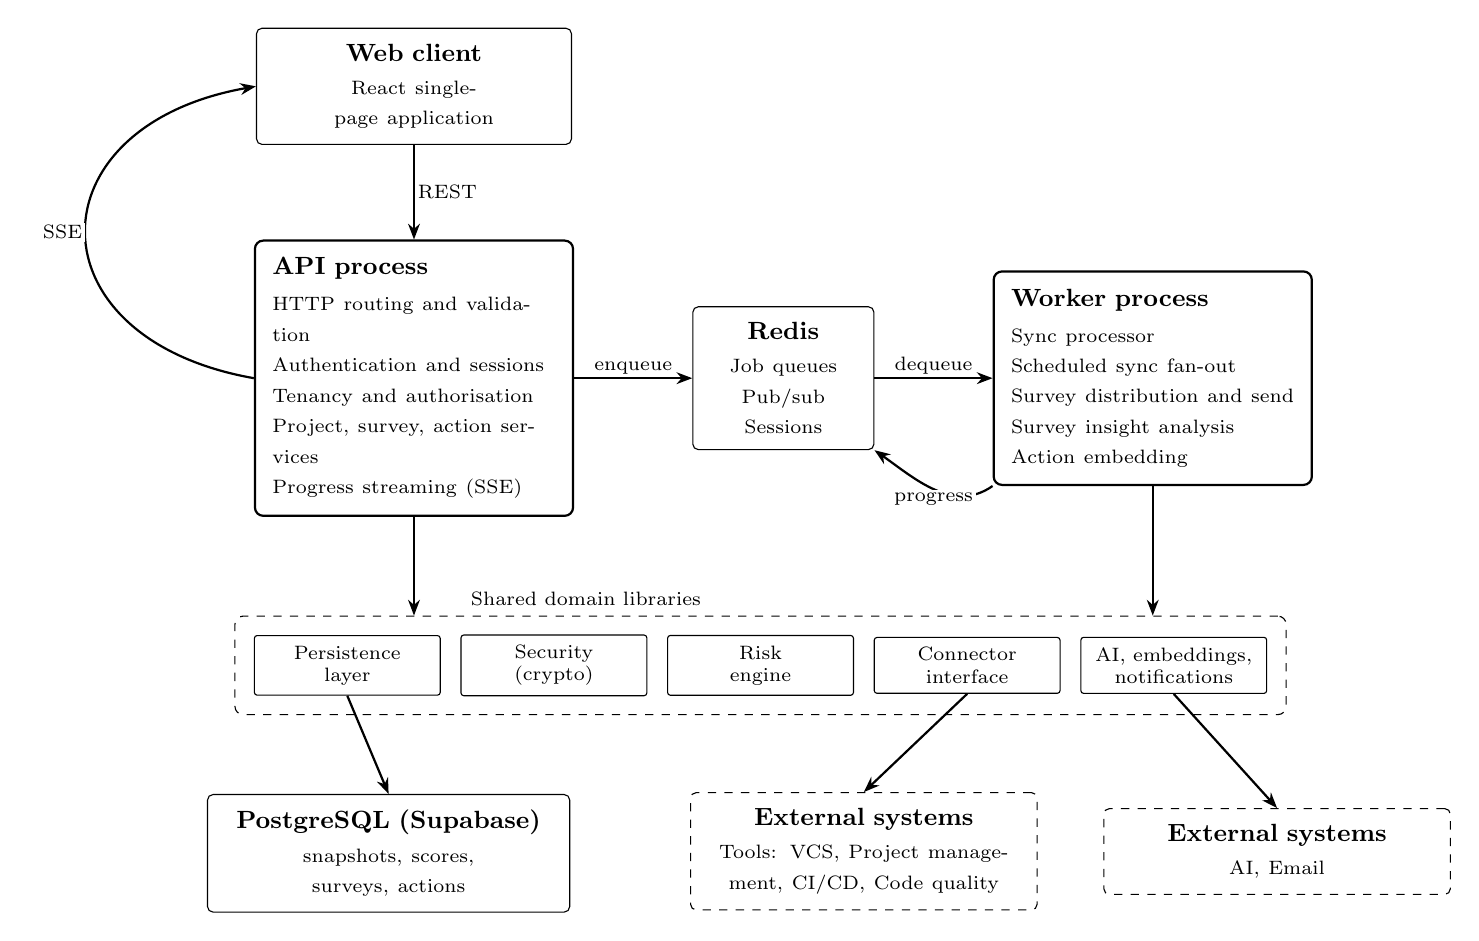
\begin{tikzpicture}[
  font=\small,
  proc/.style={draw, thick, rounded corners=3pt, align=left, inner sep=2.2mm,
               text width=36mm},
  infra/.style={draw, rounded corners=2pt, align=center, inner sep=2mm},
  chip/.style={draw, rounded corners=1pt, align=center, text width=21mm,
               inner sep=1.3mm, font=\scriptsize},
  ext/.style={draw, dashed, rounded corners=2pt, align=center, inner sep=2mm},
  band/.style={draw, dashed, rounded corners=3pt, inner sep=2.4mm},
  arr/.style={-{Stealth[length=2mm]}, thick},
  tag/.style={font=\scriptsize, fill=white, inner sep=1pt}
]

%% ---- processes ----
\node[proc] (api) at (0,0) {\textbf{API process}\\[2pt]
  {\scriptsize HTTP routing and validation}\\
  {\scriptsize Authentication and sessions}\\
  {\scriptsize Tenancy and authorisation}\\
  {\scriptsize Project, survey, action services}\\
  {\scriptsize Progress streaming (SSE)}};

\node[infra, text width=19mm, right=15mm of api] (redis) {\textbf{Redis}\\[1pt]
  {\scriptsize Job queues}\\
  {\scriptsize Pub/sub}\\
  {\scriptsize Sessions}};

\node[proc, right=15mm of redis] (worker) {\textbf{Worker process}\\[2pt]
  {\scriptsize Sync processor}\\
  {\scriptsize Scheduled sync fan-out}\\
  {\scriptsize Survey distribution and send}\\
  {\scriptsize Survey insight analysis}\\
  {\scriptsize Action embedding}};

%% ---- client ----
\node[infra, text width=36mm, above=12mm of api] (client) {\textbf{Web client}\\[1pt]
  {\scriptsize React single-page application}};

%% ---- shared domain libraries ----
\node[chip, below=15mm of api.south west, anchor=north west] (p1)
  {Persistence\\layer};
\node[chip, right=2.5mm of p1] (p2) {Security\\(crypto)};
\node[chip, right=2.5mm of p2] (p3) {Risk\\engine};
\node[chip, right=2.5mm of p3] (p4) {Connector\\interface};
\node[chip, right=2.5mm of p4] (p5) {AI, embeddings,\\notifications};

\begin{scope}[on background layer]
  \node[band, fit=(p1)(p5),
        label={[font=\scriptsize]above left:Shared domain libraries}] (libs) {};
\end{scope}

%% ---- infrastructure and external systems ----
\node[infra, text width=42mm] (db)
  at ($(p1.south)!0.2!(p2.south) + (0,-20mm)$)
  {\textbf{PostgreSQL (Supabase)}\\[1pt]
   {\scriptsize snapshots, scores, surveys, actions}};

\node[ext, text width=40mm] (extsys)
  at ($(p4.south)!-0.5!(p5.south) + (0,-20mm)$)
  {\textbf{External systems}\\[1pt]
   {\scriptsize Tools: VCS, Project management, CI/CD, Code quality}};

\node[ext, text width=40mm] (fxtsys)
  at ($(p4.south)!1.5!(p5.south) + (0,-20mm)$)
  {\textbf{External systems}\\[1pt]
   {\scriptsize AI, Email}};

%% ---- flows ----
\draw[arr] (client) -- node[tag, right] {REST} (api);
\draw[arr] (api.west) to[out=170, in=190, looseness=2]
  node[tag, left] {SSE} (client.west);

\draw[arr] (api) -- node[tag, above] {enqueue} (redis);
\draw[arr] (redis) -- node[tag, above] {dequeue} (worker);
\draw[arr] (worker.south west) to[out=215, in=325]
  node[tag, below] {progress} (redis.south east);

\draw[arr] (api.south) -- (api.south |- libs.north);
\draw[arr] (worker.south) -- (worker.south |- libs.north);

\draw[arr] (p1.south) -- (db.north);
\draw[arr] (p4.south) -- (extsys.north);
\draw[arr] (p5.south) -- (fxtsys.north);
\end{tikzpicture}
\caption{System architecture. The API process serves the client synchronously and
the worker performs all long-running and scheduled work; Redis carries both the
job queues between them and the progress events flowing back. Both processes draw
on the same domain libraries, which are the only components that contact the
database or external systems.}
\label{fig:architecture}
\end{figure}


\subsection{Rationale for the Partition}
\label{subsec:partition-rationale}

Splitting the API and worker into separate processes follows from the nature of
the work. A single synchronisation queries four external APIs, some with
pagination over hundreds of records, and can run for minutes. Performing that
inside a request would hold the connection open far beyond any reasonable
timeout, and a failure part-way through would leave the user with an error and no
record of the partial work. Moving it to a worker allows the request to return
immediately with an acknowledgement, and allows the work itself to be retried,
prioritised and rate-limited independently of any user waiting on it (NFR-11,
NFR-16).

That separation creates a problem of its own: the worker performs the work, but
only the API process holds a connection to the user's browser, so the worker
cannot report progress directly. Redis resolves this by carrying both directions
of the exchange. It holds the job queues through which the API hands work to the
worker, and it carries a publish/subscribe channel per synchronisation session
through which the worker reports progress back. The API subscribes to that
channel and relays each event to the browser over Server-Sent Events. The final
completion event is additionally retained in Redis for a limited period, so that a
client which reloads the page after a synchronisation has finished still receives
its outcome rather than waiting on a channel that will never speak again
(FR-17).

\subsection{Module Responsibilities}
\label{subsec:module-responsibilities}

\begin{longtable}{
  >{\raggedright\arraybackslash}p{0.24\textwidth}
  >{\raggedright\arraybackslash}p{0.34\textwidth}
  >{\raggedright\arraybackslash}p{0.28\textwidth}
}
\caption{Modules, their responsibilities and principal interactions}
\label{tab:modules}\\
\toprule
\textbf{Module} & \textbf{Responsibility} & \textbf{Interacts with} \\
\midrule
\endfirsthead
\toprule
\textbf{Module} & \textbf{Responsibility} & \textbf{Interacts with} \\
\midrule
\endhead
\bottomrule
\endlastfoot
Web client & Presents the portfolio, dashboards, settings and survey interfaces;
consumes the progress stream & API process \\
\addlinespace
HTTP interface layer & Routes requests, validates input, maps domain errors to status
codes & All API-side services \\
\addlinespace
Authentication and session management & Verifies credentials, issues and revokes
sessions, manages verification, invitation and reset tokens & Redis session store,
user data access \\
\addlinespace
Authorisation and tenancy & Restricts every access to the caller's company, and
further to assigned projects for non-administrators & All API-side services \\
\addlinespace
Project and workspace services & Repository import, tool integration configuration,
member management & Data access, connector repository listing \\
\addlinespace
Progress streaming & Subscribes to a session's event channel and relays events to the
browser & Redis pub/sub \\
\addlinespace
Queue abstraction & Declares the job queues, their retry, priority and retention
policies, and the scheduler & API process, worker process, Redis \\
\addlinespace
Sync processor & Orchestrates one synchronisation: fetch, persist, score, report &
Connectors, persistence, risk engine, event store \\
\addlinespace
Scheduled sync fan-out & Expands a scheduler tick into one queued job per project,
staggered by shared credential & Queue abstraction, project data access \\
\addlinespace
Survey processors & Assign monthly pulses, generate questions, dispatch links,
analyse responses on close & AI client, notification clients, survey data access \\
\addlinespace
Connector interface & Presents one interface per tool category; each provider
implementation converts a vendor API into a normalised metric object & Worker
process, external tool APIs \\
\addlinespace
Risk engine & Converts a normalised metric set into the seven health scores, with
weights and null handling & Sync processor, survey health context \\
\addlinespace
AI client abstraction & Question generation, question scoring and response analysis
behind a provider-independent interface & Survey processors \\
\addlinespace
Embedding and search & Produces and stores action vectors; performs semantic
retrieval and reranking & Action services, worker process \\
\addlinespace
Security module & Credential encryption at rest and survey link sealing & Data access
layer, survey dispatch \\
\addlinespace
Notification clients & Delivers survey links to team channels and transactional email
& Survey processors \\
\addlinespace
Persistence layer & All database access, with encryption and decryption applied at
this boundary & Every module above \\
\end{longtable}

Three of these boundaries carry most of the design's extensibility, and are worth
stating explicitly.

The \textbf{connector interface} is what satisfies O-07 and NFR-21. Each
provider implements a single method returning a normalised metric object, and a
registry maps a tool name to its implementation. Nothing downstream of that
interface, not the sync processor, not the persistence layer, not the risk
engine, contains any provider-specific logic. Adding a new version-control
provider is therefore the addition of one class and one registry entry.

The \textbf{risk engine} isolates scoring behind a similar boundary. Each of the
seven dimensions is an independent strategy selected by an enumeration, and every
strategy is built from the same shared set of normalisation functions and a
common null-aware weighting routine. A dimension's rules can be changed, or a
dimension added, without touching ingestion or presentation which is a property that
was exercised in practice when the scoring model was revised, as described in
\Cref{sec:detailed-design}.

The \textbf{persistence layer} is the single point at which credential encryption
is applied. Encryption occurs on write and decryption on read, both inside the
data-access functions, so that every module above this boundary operates on
plaintext and none of them can accidentally persist an unencrypted credential.

\subsection{Interaction: The Synchronisation Path}
\label{subsec:interaction-sync}

The synchronisation flow exercises most of the system and illustrates how the
modules cooperate. A request arrives at the HTTP layer, which validates it and
confirms through the authorisation module that the caller may act on the named
project. The project service resolves the configured integrations, decrypting
each credential at the persistence boundary and resolving the version-control
token from the owning workspace where the project does not carry its own. The
queue abstraction enqueues a job carrying the project, the tool list and the
session identifier, and the request returns an acknowledgement.

The worker dequeues the job and creates one snapshot record for the run. It then
fetches from the configured tools concurrently, subject to a concurrency bound
(NFR-15), publishing a progress event as each tool begins and finishes. Each
tool's normalised output is written against the shared snapshot. A tool that
fails is recorded as failed and the run continues (FR-19, NFR-10). Once
persistence is complete, the risk engine computes the seven scores from whatever
metrics the snapshot actually contains, redistributing the weight of absent
inputs (FR-22), and the scores are stored against the snapshot. A completion
event is published and retained. Throughout, the API process has been relaying
each published event to the browser, which updates per-tool status in place.

\subsection{Influence of Standards and Codes of Practice}
\label{subsec:standards-in-design}

The obligations established in \Cref{sec:standards} were not applied as a review
performed after construction; several of them determined where module boundaries
were drawn in the first place. \Cref{tab:standards-design} records where each
one is realised in the structure.

\begin{longtable}{
  >{\raggedright\arraybackslash}p{0.26\textwidth}
  >{\raggedright\arraybackslash}p{0.60\textwidth}
}
\caption{Where the standards of \Cref{sec:standards} shaped the design}
\label{tab:standards-design}\\
\toprule
\textbf{Obligation} & \textbf{Effect on the design} \\
\midrule
\endfirsthead
\toprule
\textbf{Obligation} & \textbf{Effect on the design} \\
\midrule
\endhead
\bottomrule
\endlastfoot
Access control (OWASP A01) & Tenancy scoping is applied inside the persistence layer
rather than in individual handlers, so that a query cannot omit it by oversight. Role
and project-membership checks sit in the service layer, above it \\
\addlinespace
Cryptographic protection (OWASP A02) & All cryptography is confined to a single
security module, and applied at the persistence boundary. No other module performs
encryption, which keeps the algorithm, key handling and versioning in one auditable
place \\
\addlinespace
Injection resistance (OWASP A03) & A single parameterised data-access client is the
only route to the database; no module composes SQL. One shared helper sanitises
user-supplied search terms, and one escapes values placed into outgoing email \\
\addlinespace
Abuse resistance (OWASP A04) & Rate limiting is applied as middleware at the router
handling unauthenticated requests. Dispatch quotas and recipient cooldowns are
enforced inside the survey dispatch module, not at the call sites that invoke it \\
\addlinespace
Respondent anonymity (NFR-07) & Enforced structurally rather than procedurally: the
survey response table carries no foreign key to a user, so no query can reconstruct
the association. The design places the guarantee in the schema, where application
code cannot circumvent it \\
\addlinespace
Data minimisation & The AI client abstraction is the only module permitted to
transmit data externally for analysis, and the prompt-construction layer strips
personal names and work-item identifiers before transmission, giving a single
chokepoint to audit \\
\addlinespace
Temporal correctness (ISO 8601, RFC 3339) & Timestamp parsing and formatting are
centralised in a shared utility, and the database columns were migrated to zone-aware
types so that instants are unambiguous regardless of the reader's locale \\
\addlinespace
Accessibility (WCAG 2.1 AA) & Interactive elements in the client are built from
shared components that carry role, focus and keyboard behaviour by default, so that
accessibility properties are inherited rather than reapplied per screen \\
\end{longtable}

\subsection{Health, Safety and Environmental Considerations}
\label{subsec:hse-design}

The system performs no physical actuation and controls no equipment, so the
safety considerations that govern cyber-physical systems do not arise. Two
related considerations do apply, and both influenced the design.

The first concerns \textbf{occupational wellbeing}. The system measures the work
of identifiable people, and a monitoring tool of this kind can readily become an
instrument of individual performance assessment with predictable effects on
the behaviour of those measured. Three design decisions deliberately foreclose
that use. Metrics are aggregated to the project level and no per-developer view
exists anywhere in the interface, despite the underlying data making one
technically feasible. Qualitative feedback is anonymous by schema construction,
as described above, so that candour carries no personal risk. And survey dispatch
is bounded by per-project quotas and per-recipient cooldowns, so that
participation does not itself become a burden. These constraints resolve the
conflict between managerial visibility and developer psychological safety
identified in \Cref{subsec:conflicts}, and they are properties of the design rather
than matters of policy.

The second concerns \textbf{resource consumption}. Two choices reduce it
materially. Collection is scheduled rather than continuous, so the system issues
a bounded number of external requests per project per day instead of polling,
and projects sharing a credential are staggered, which flattens the load profile
rather than concentrating it. Both were adopted primarily to respect third-party
rate limits and free-tier quotas, but their effect on energy and network
consumption is the same. The resources the deployment consumes are quantified in
\Cref{sec:deployment}, and their environmental impact assessed in
\Cref{sec:sustainability}.

% \section{Design Refinement and Simulation}
% \label{sec:detailed-design}
% \guidance{Present the detailed design using the views that fit the project (ERD,
% class, sequence, DFD, API, wireframes, circuit, model). Include any design
% calculations or estimates made (e.g. expected load or storage), the
% analyses, prototypes, or simulations used to verify the design against the
% requirements, and how the design was refined to facilitate implementation.}


\section{Design Refinement and Simulation}
\label{sec:detailed-design}

This section presents the detailed design through the views that carry the most
information about this system such as the structure of the two extensible layers, the
data model, the synchronisation sequence, and the external interface. It then
records the storage and load estimates made during design, the means by which the
design was checked against its requirements, and the refinements made to the
design during implementation.

\subsection{Structure of the Connector and Scoring Layers}
\label{subsec:connector-scoring-structure}

\Cref{fig:connector-scoring} shows the internal structure of the two layers that
carry the system's extensibility, and the path by which data travels from one to
the other. External tool APIs are omitted here; they appear in
\Cref{fig:architecture}.

\begin{figure}[htbp]
\centering
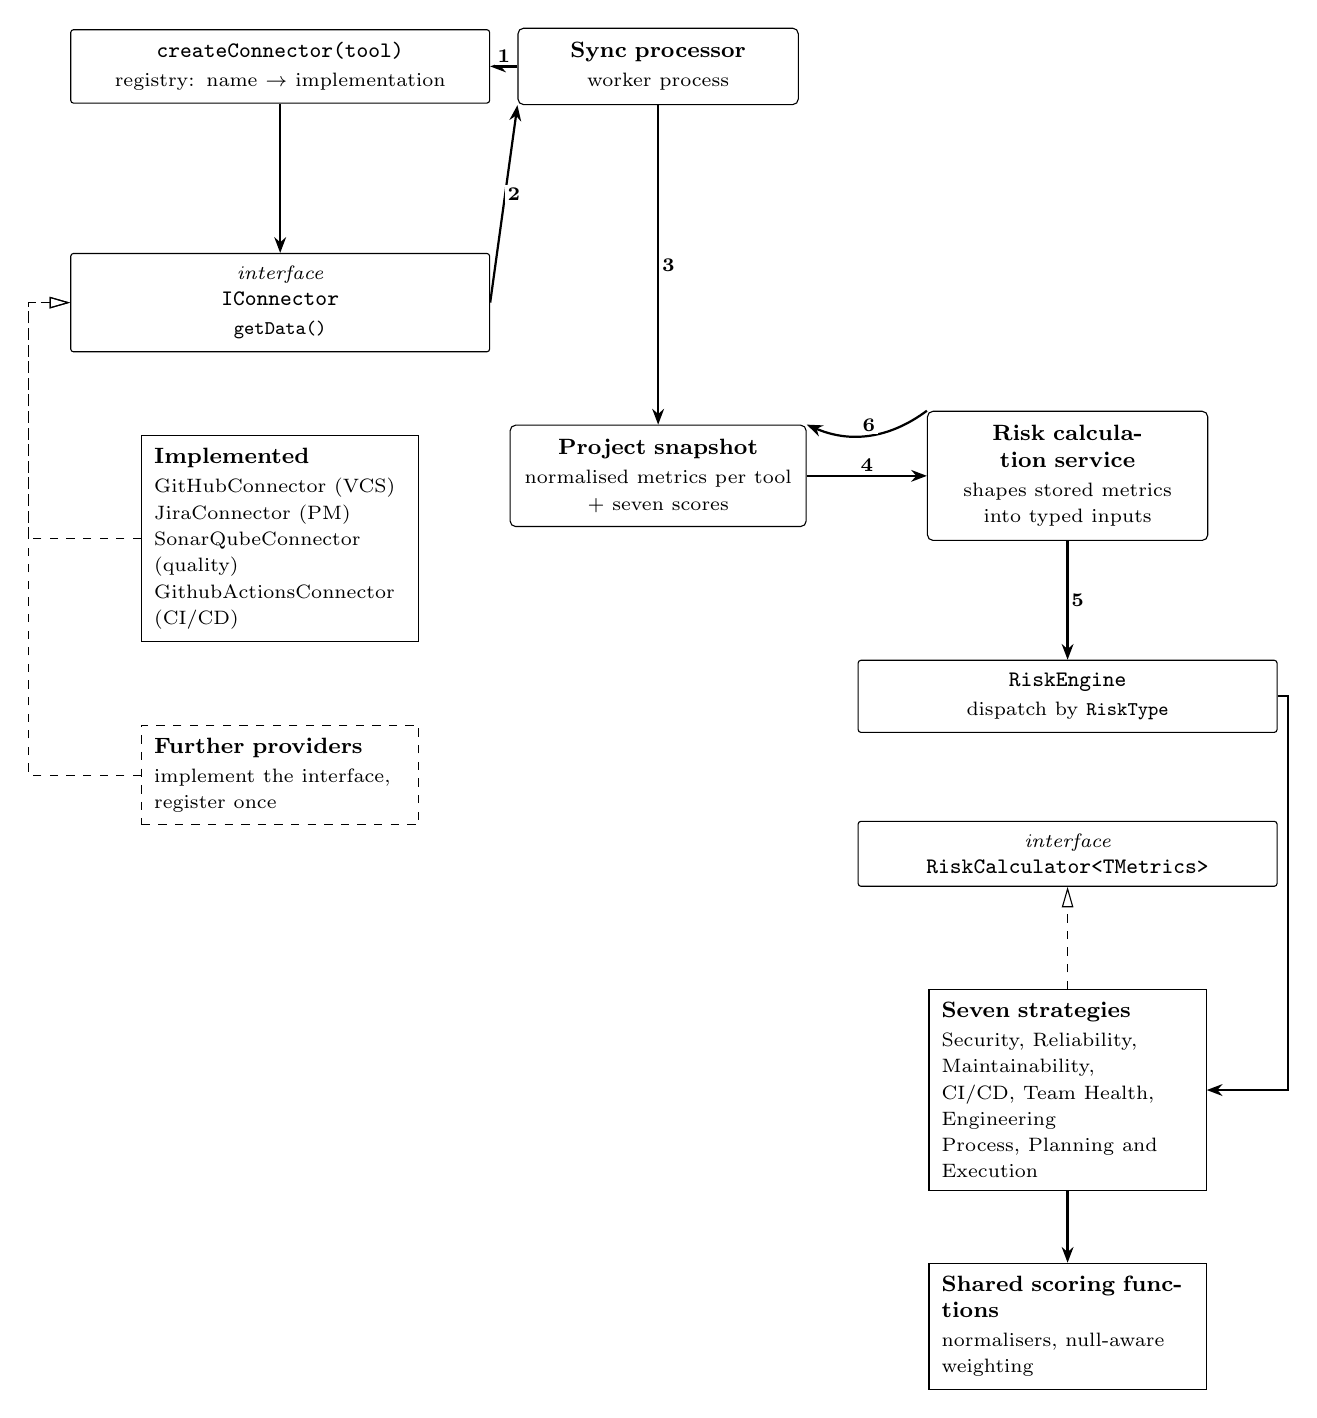
\begin{tikzpicture}[
  font=\footnotesize,
  iface/.style={draw, rounded corners=1pt, align=center, text width=50mm,
                inner sep=1.6mm},
  cls/.style={draw, align=left, text width=32mm, inner sep=1.6mm},
  ghost/.style={draw, dashed, align=left, text width=32mm, inner sep=1.6mm},
  store/.style={draw, rounded corners=2pt, align=center, text width=32mm,
                inner sep=1.8mm},
  arr/.style={-{Stealth[length=2mm]}, thick},
  real/.style={-{Triangle[open, length=2.6mm]}, dashed, thin},
  % step/.style={font=\scriptsize\bfseries, fill=white, inner sep=1pt}
  flowstep/.style={font=\scriptsize\bfseries, fill=white, inner sep=1pt}
]


%% ---------- centre: worker and store ----------
\node[store] (proc) at (0mm,0mm) {\textbf{Sync processor}\\[1pt]
  {\scriptsize worker process}};
\node[store, text width=34mm] (snap) at (0mm,-52mm)
  {\textbf{Project snapshot}\\[1pt]
   {\scriptsize normalised metrics per tool}\\
   {\scriptsize + seven scores}};

%% ---------- left: connector layer ----------
\node[iface] (reg) at (-48mm,0mm) {\texttt{createConnector(tool)}\\[1pt]
  {\scriptsize registry: name $\rightarrow$ implementation}};
\node[iface] (iface) at (-48mm,-30mm)
  {{\scriptsize\itshape interface}\\ \texttt{IConnector}\\[1pt]
   {\scriptsize \texttt{getData()}}};
\node[cls] (impl) at (-48mm,-60mm) {\textbf{Implemented}\\[1pt]
  {\scriptsize GitHubConnector (VCS)}\\
  {\scriptsize JiraConnector (PM)}\\
  {\scriptsize SonarQubeConnector (quality)}\\
  {\scriptsize GithubActionsConnector (CI/CD)}};
\node[ghost] (future) at (-48mm,-90mm) {\textbf{Further providers}\\[1pt]
  {\scriptsize implement the interface, register once}};

%% ---------- right: scoring layer ----------
\node[store] (rcs) at (52mm,-52mm) {\textbf{Risk calculation service}\\[1pt]
  {\scriptsize shapes stored metrics into typed inputs}};
\node[iface] (engine) at (52mm,-80mm) {\texttt{RiskEngine}\\[1pt]
  {\scriptsize dispatch by \texttt{RiskType}}};
\node[iface] (rcalc) at (52mm,-100mm)
  {{\scriptsize\itshape interface}\\ \texttt{RiskCalculator<TMetrics>}};
\node[cls] (strat) at (52mm,-130mm) {\textbf{Seven strategies}\\[1pt]
  {\scriptsize Security, Reliability, Maintainability,}\\
  {\scriptsize CI/CD, Team Health, Engineering}\\
  {\scriptsize Process, Planning and Execution}};
\node[cls] (util) at (52mm,-160mm) {\textbf{Shared scoring functions}\\[1pt]
  {\scriptsize normalisers, null-aware weighting}};

%% ---------- realisation: orthogonal spine at x = -70mm ----------
\draw[real] (impl.west)   -- (-80mm,-60mm)  -- (-80mm,-30mm) -- (iface.west);
% \draw[real] (stub.west)   -- (-70mm,-90mm)  -- (-70mm,-30mm) -- (iface.west);
\draw[real] (future.west) -- (-80mm,-90mm) -- (-80mm,-30mm) -- (iface.west);
\draw[real] (strat.north) -- (rcalc.south);

%% ---------- flow ----------
\draw[arr] (proc.west) -- node[flowstep, above] {1} (reg.east);
\draw[arr] (reg.south) -- (iface.north);
\draw[arr] (iface.east) -- node[flowstep, above right] {2} (proc.south west);
\draw[arr] (proc.south) -- node[flowstep, right] {3} (snap.north);
\draw[arr] (snap.east) -- node[flowstep, above] {4} (rcs.west);
\draw[arr] (rcs.south) -- node[flowstep, right] {5} (engine.north);
\draw[arr] (engine.east) -- (80mm,-80mm) -- (80mm,-130mm) -- (strat.east);
\draw[arr] (strat.south) -- (util.north);
\draw[arr] (rcs.north west) to[bend left=30]
  node[flowstep, above] {6} (snap.north east);
\end{tikzpicture}

\caption{Structure of the connector and scoring layers. The worker depends only
on the \texttt{IConnector} interface, never on a specific provider (1--2);
normalised metrics are written to the snapshot (3) and read back from it for
scoring (4--6), so the two layers never reference each other directly.}
\label{fig:connector-scoring}
\end{figure}

\paragraph{The connector extension point.}
Every provider implementation satisfies one interface, \texttt{IConnector},
declaring a single method that returns a normalised metric object. A registry maps
each supported tool name to the function that constructs its implementation, and
the sync processor obtains a connector only through that registry. The
consequence is that the worker contains no reference to any specific provider, 
it names a tool, receives something satisfying the interface, and calls one method
on it. Provider-specific concerns, GitHub's separate REST and GraphQL rate
budgets, Jira's instance-specific custom field identifiers, SonarQube's paginated
measure history, are confined entirely within their own implementations.

Adding a provider therefore costs one class and one registry entry, with no
change to the sync processor, the persistence layer or the scoring engine. This
is what satisfies O-07 and NFR-21.

\paragraph{Decoupling of ingestion from scoring.}
The connector layer and the risk engine never communicate directly. The worker
writes each tool's normalised output to the project snapshot, and the risk
calculation service subsequently reads those stored metrics back out, shapes them
into the typed input object each strategy expects, and invokes the engine. The
snapshot is the integration point between ingestion and scoring.

This indirection is deliberate, and it buys three properties. Scoring becomes
reproducible. Since the inputs are stored rather than consumed in flight, a
score can be recomputed at any later time from the snapshot that produced it,
without contacting any external tool, which is how the per-metric score
breakdown of FR-26 is served months after the data was collected. Scoring also
becomes independently revisable. The weighting rules can change and be re-applied
to historical snapshots, because the raw evidence was retained. And a failure in
either layer is harmless to the other. A connector fault costs one tool's metrics for one
snapshot, while a scoring fault leaves the ingested data intact for later
recomputation.

\paragraph{The scoring extension point.}
The risk engine mirrors the connector layer's shape. Each of the seven dimensions
is an independent strategy implementing \texttt{RiskCalculator<TMetrics>},
generic in the metric type it consumes, and the engine dispatches to the
appropriate one by enumeration member. Each strategy declares its inputs as a
list of weighted signals and delegates the arithmetic to a shared set of
normalisation functions and a common null-aware weighting routine, so that the
behaviour on missing data (FR-22) is implemented once and identically for every
dimension rather than restated seven times.

A dimension's weights or thresholds can therefore be changed by editing one
strategy, and a dimension can be added by writing one class and one enumeration
member. That this holds in practice was demonstrated during development, when the
scoring model was restructured from six categories to seven, the change was
confined to the strategy layer and the score persistence schema, leaving
ingestion, the queue, the progress stream and the client untouched.


\subsection{Data Model}
\label{subsec:data-model}

The schema comprises seventeen tables, presented here in three related views:
tenancy and project structure (\Cref{fig:erd-tenancy}), metric capture and
scoring (\Cref{fig:erd-metrics}), and team engagement (\Cref{fig:erd-engagement}).
The \texttt{project} entity appears in all three, as it is the point on which
every other concern hangs.

\begin{figure}[htbp]
\centering
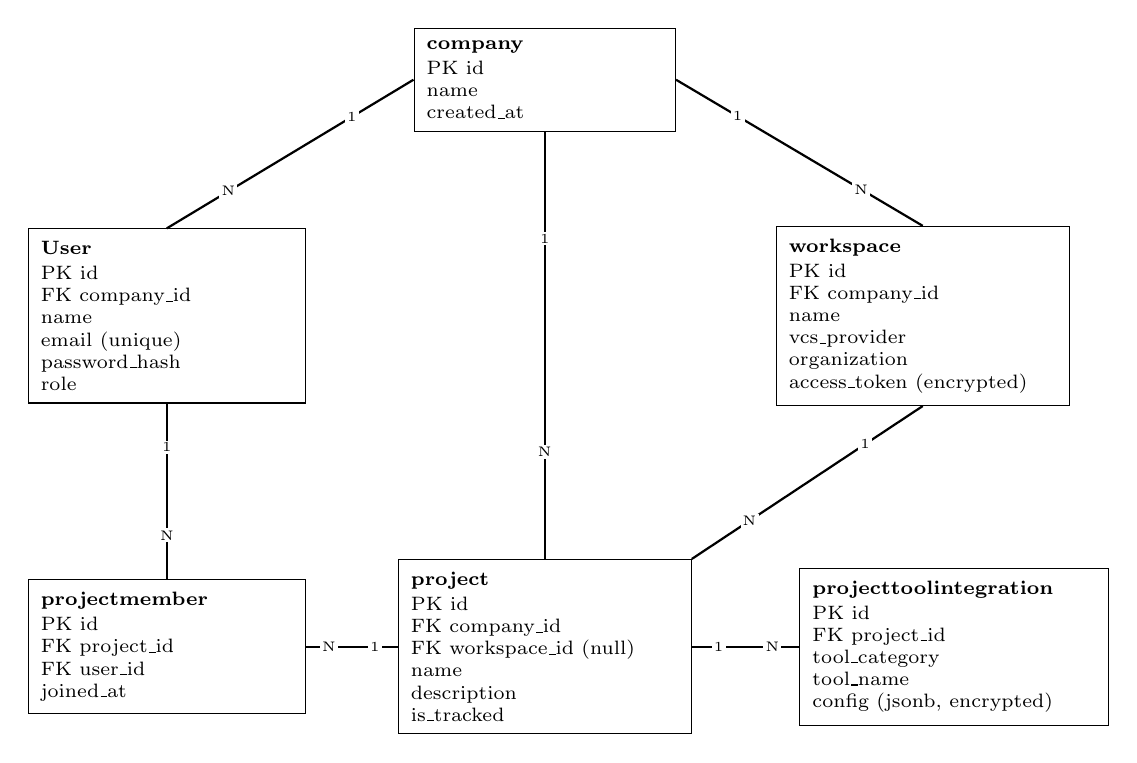
\begin{tikzpicture}[
  font=\scriptsize,
  ent/.style={draw, align=left, inner sep=1.6mm},
  rel/.style={thick},
  card/.style={font=\tiny, fill=white, inner sep=0.8pt}
]
\node[ent, text width=30mm] (co) at (0mm,0mm)
  {\textbf{company}\\[1pt] PK id\\ name\\ created\_at};

\node[ent, text width=32mm] (usr) at (-48mm,-30mm)
  {\textbf{User}\\[1pt] PK id\\ FK company\_id\\ name\\ email (unique)\\
   password\_hash\\ role};

\node[ent, text width=34mm] (ws) at (48mm,-30mm)
  {\textbf{workspace}\\[1pt] PK id\\ FK company\_id\\ name\\ vcs\_provider\\
   organization\\ access\_token (encrypted)};

\node[ent, text width=32mm] (pm) at (-48mm,-72mm)
  {\textbf{projectmember}\\[1pt] PK id\\ FK project\_id\\ FK user\_id\\ joined\_at};

\node[ent, text width=34mm] (proj) at (0mm,-72mm)
  {\textbf{project}\\[1pt] PK id\\ FK company\_id\\ FK workspace\_id (null)\\
   name\\ description\\ is\_tracked};

\node[ent, text width=36mm] (pti) at (52mm,-72mm)
  {\textbf{projecttoolintegration}\\[1pt] PK id\\ FK project\_id\\ tool\_category\\
   tool\_name\\ config (jsonb, encrypted)};

\draw[rel] (co.west) -- node[card, near start] {1} node[card, near end] {N}
(usr.north);
\draw[rel] (co.east) -- node[card, near start] {1} node[card, near end] {N}
(ws.north);
\draw[rel] (co.south) -- node[card, near start] {1} node[card, near end] {N}
(proj.north);
\draw[rel] (ws.south) -- node[card, near start] {1} node[card, near end] {N}
(proj.north east);
\draw[rel] (usr.south) -- node[card, near start] {1} node[card, near end] {N}
(pm.north);
\draw[rel] (proj.west) -- node[card, near start] {1} node[card, near end] {N}
(pm.east);
\draw[rel] (proj.east) -- node[card, near start] {1} node[card, near end] {N}
(pti.west);
\end{tikzpicture}
\caption{Tenancy and project structure. Every entity is owned by a company, which
is the tenancy boundary enforced on all data access.}
\label{fig:erd-tenancy}
\end{figure}

\begin{figure}[htbp]
\centering
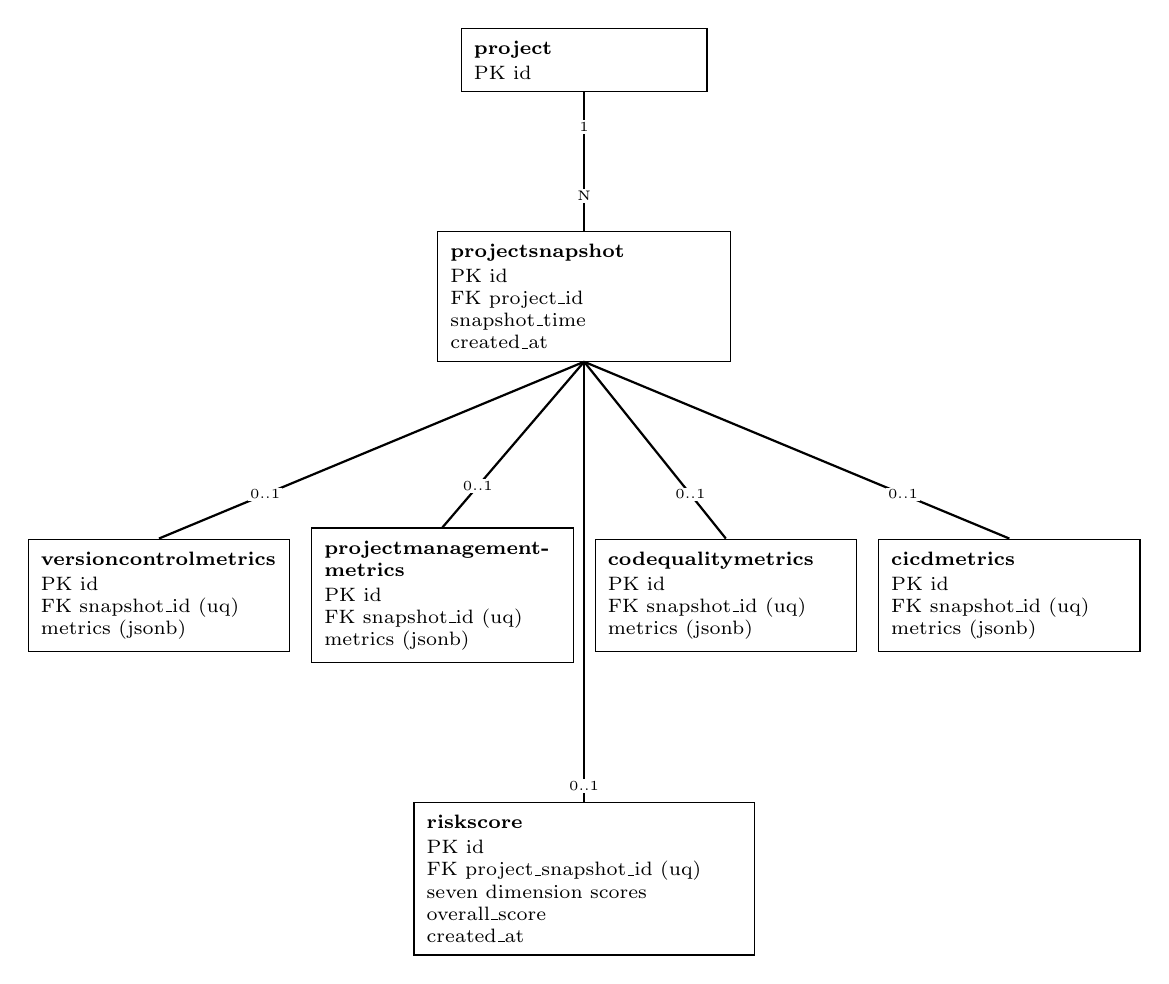
\begin{tikzpicture}[
  font=\scriptsize,
  ent/.style={draw, align=left, inner sep=1.6mm},
  rel/.style={thick},
  card/.style={font=\tiny, fill=white, inner sep=0.8pt}
]
\node[ent, text width=28mm] (proj) at (0mm,0mm)
  {\textbf{project}\\[1pt] PK id};

\node[ent, text width=34mm] (snap) at (0mm,-30mm)
  {\textbf{projectsnapshot}\\[1pt] PK id\\ FK project\_id\\ snapshot\_time\\
created\_at};

\node[ent, text width=30mm] (vcm) at (-54mm,-68mm)
  {\textbf{versioncontrolmetrics}\\[1pt] PK id\\ FK snapshot\_id (uq)\\ metrics
(jsonb)};
\node[ent, text width=30mm] (pmm) at (-18mm,-68mm)
  {\textbf{projectmanagement\-metrics}\\[1pt] PK id\\ FK snapshot\_id (uq)\\ metrics
(jsonb)};
\node[ent, text width=30mm] (cqm) at (18mm,-68mm)
  {\textbf{codequalitymetrics}\\[1pt] PK id\\ FK snapshot\_id (uq)\\ metrics
(jsonb)};
\node[ent, text width=30mm] (cicd) at (54mm,-68mm)
  {\textbf{cicdmetrics}\\[1pt] PK id\\ FK snapshot\_id (uq)\\ metrics (jsonb)};

\node[ent, text width=40mm] (risk) at (0mm,-104mm)
  {\textbf{riskscore}\\[1pt] PK id\\ FK project\_snapshot\_id (uq)\\
   seven dimension scores\\ overall\_score\\ created\_at};

\draw[rel] (proj.south) -- node[card, near start] {1} node[card, near end] {N}
(snap.north);
\draw[rel] (snap.south) -- node[card, near end] {0..1} (vcm.north);
\draw[rel] (snap.south) -- node[card, near end] {0..1} (pmm.north);
\draw[rel] (snap.south) -- node[card, near end] {0..1} (cqm.north);
\draw[rel] (snap.south) -- node[card, near end] {0..1} (cicd.north);
\draw[rel] (snap.south) -- (0mm,-86mm) -- node[card, near end] {0..1} (risk.north);
\end{tikzpicture}
\caption{Metric capture and scoring. A snapshot is an immutable record of one
synchronisation; the unique constraint on each child table admits at most one row
per snapshot per tool, and a snapshot for which a tool was unconfigured or failed
simply has no corresponding row.}
\label{fig:erd-metrics}
\end{figure}

\begin{figure}[htbp]
\centering
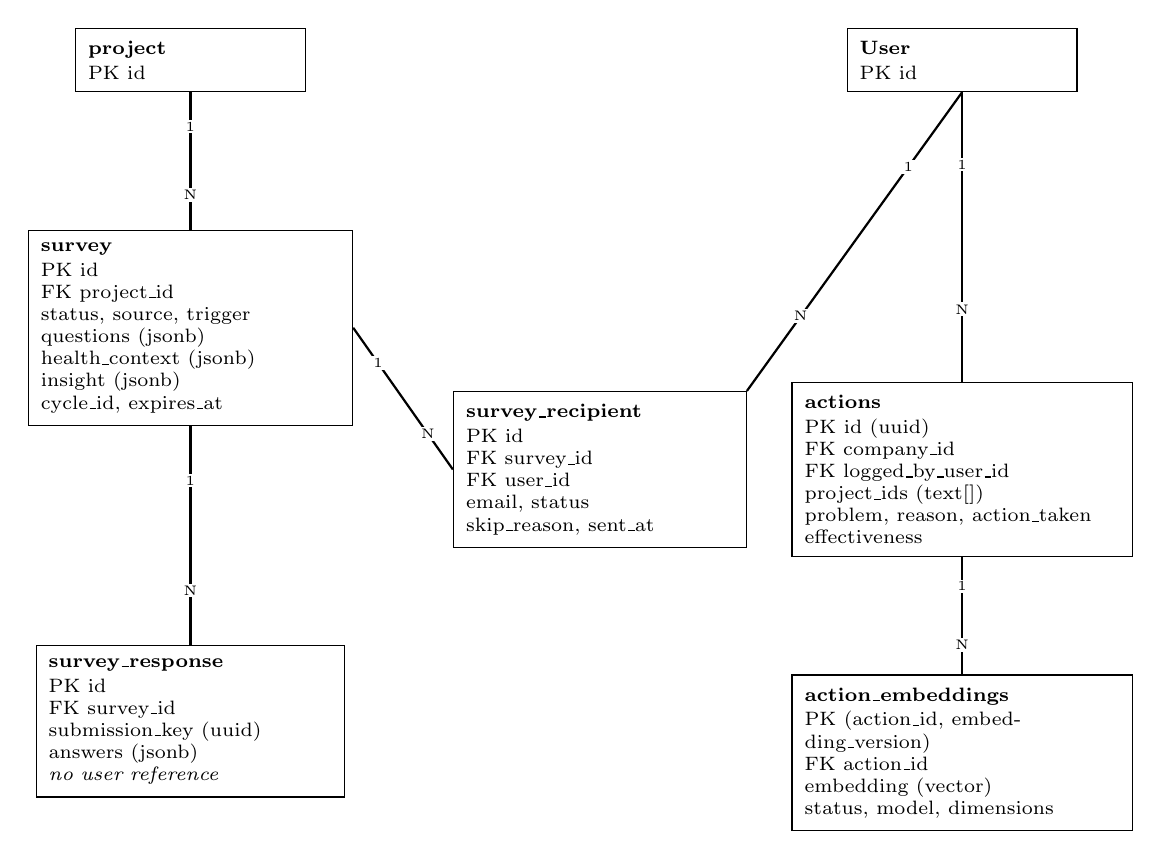
\begin{tikzpicture}[
  font=\scriptsize,
  ent/.style={draw, align=left, inner sep=1.6mm},
  rel/.style={thick},
  weak/.style={thick, dashed},
  card/.style={font=\tiny, fill=white, inner sep=0.8pt}
]
\node[ent, text width=26mm] (proj) at (-52mm,0mm)
  {\textbf{project}\\[1pt] PK id};
\node[ent, text width=26mm] (usr) at (46mm,0mm)
  {\textbf{User}\\[1pt] PK id};

\node[ent, text width=38mm] (srv) at (-52mm,-34mm)
  {\textbf{survey}\\[1pt] PK id\\ FK project\_id\\ status, source, trigger\\
   questions (jsonb)\\ health\_context (jsonb)\\ insight (jsonb)\\
   cycle\_id, expires\_at};

\node[ent, text width=36mm] (resp) at (-52mm,-84mm)
  {\textbf{survey\_response}\\[1pt] PK id\\ FK survey\_id\\ submission\_key (uuid)\\
   answers (jsonb)\\ \emph{no user reference}};

\node[ent, text width=34mm] (rcp) at (0mm,-52mm)
  {\textbf{survey\_recipient}\\[1pt] PK id\\ FK survey\_id\\ FK user\_id\\
   email, status\\ skip\_reason, sent\_at};

\node[ent, text width=40mm] (act) at (46mm,-52mm)
  {\textbf{actions}\\[1pt] PK id (uuid)\\ FK company\_id\\ FK logged\_by\_user\_id\\
   project\_ids (text[])\\ problem, reason, action\_taken\\ effectiveness};

\node[ent, text width=40mm] (emb) at (46mm,-88mm)
  {\textbf{action\_embeddings}\\[1pt] PK (action\_id, embedding\_version)\\
   FK action\_id\\ embedding (vector)\\ status, model, dimensions};

\draw[rel] (proj.south) -- node[card, near start] {1} node[card, near end] {N}
(srv.north);
\draw[rel] (srv.south) -- node[card, near start] {1} node[card, near end] {N}
(resp.north);
\draw[rel] (srv.east) -- node[card, near start] {1} node[card, near end] {N}
(rcp.west);
\draw[rel] (usr.south) -- node[card, near start] {1} node[card, near end] {N}
(rcp.north east);
\draw[rel] (usr.south) -- node[card, near start] {1} node[card, near end] {N}
(act.north);
\draw[rel] (act.south) -- node[card, near start] {1} node[card, near end] {N}
(emb.north);
% \draw[weak] (proj.north) -- (-52mm,14mm) -- (46mm,14mm)
%   node[card, midway, above] {referenced by value, not by key} (act.north west);
\end{tikzpicture}
\caption{Surveys and management actions. Two relationships are deliberately
absent as foreign keys: a survey response holds no reference to the respondent,
and an action names its projects in a text array rather than through a join
table.}
\label{fig:erd-engagement}
\end{figure}

\paragraph{Immutable snapshots.}
The central structural decision is that a synchronisation produces an
append-only record. A \texttt{projectsnapshot} row is created per run, each
tool's output is attached to it, and the computed scores are attached to the same
row; nothing is ever updated in place. Trend data is therefore a by-product of
the storage model rather than a separate concern, and any historical score
remains attributable to the exact inputs that produced it which is what makes
the on-demand score breakdown of FR-26 possible.

\paragraph{Semi-structured metric storage.}
Each of the four metric tables holds a single \texttt{jsonb} column rather than a
column per metric. This was a revision made during implementation, discussed in
\Cref{subsec:design-refinement}, and it reflects the reality that each connector
returns a deeply nested, provider-specific structure which evolves as a
connector's coverage improves. Relational columns would have required a schema
migration for every metric added, whereas the scoring layer reads the fields it
needs by name and tolerates their absence by design (FR-22).

\paragraph{Anonymity enforced structurally.}
\texttt{survey\_response} carries a randomly generated \texttt{submission\_key}
and no reference to any user. The system records separately, in
\texttt{survey\_recipient}, who was invited to a survey, but there is no
column anywhere linking an invitation to a response. The anonymity guarantee of
NFR-07 is therefore a property of the schema, not of application logic. No query
can reconstruct the association, and no future change to the service layer can
accidentally expose it.

\paragraph{Actions referenced by value.}
An action names the projects it concerns in a \texttt{text[]} column rather than
through a join table. This is a deliberate denormalisation. An action is a
managerial narrative that may span several projects, is queried almost
exclusively by containment, and carries no per-project attributes that a join
table would hold. The cost is the loss of referential integrity to
\texttt{project}, which the application compensates for by validating project
membership at write time.

\paragraph{Versioned embeddings.}
\texttt{action\_embeddings} is keyed on the pair
\texttt{(action\_id, embedding\_version)} rather than on the action alone, so that
vectors produced by different models or dimensionalities coexist. This permits an
embedding model to be replaced by generating a new version alongside the old one
and switching over once backfill completes, rather than by a destructive
migration. This capability was exercised when the embedding provider was
changed during development.


\subsection{Synchronisation Sequence}
\label{subsec:sync-sequence}

\Cref{fig:sync-sequence} traces one user-initiated synchronisation from the
button press to the updated dashboard. The client opens its progress stream before submitting
the synchronisation request, so that events emitted by a fast connector cannot
occur in the gap between the request returning and the stream being established.
No progress event travels directly from the worker to the browser. The
worker performs the work but holds no connection to the client, so every event is
published to Redis, relayed by the API process, and forwarded over Server-Sent
Events.

\begin{figure}[htbp]
\centering
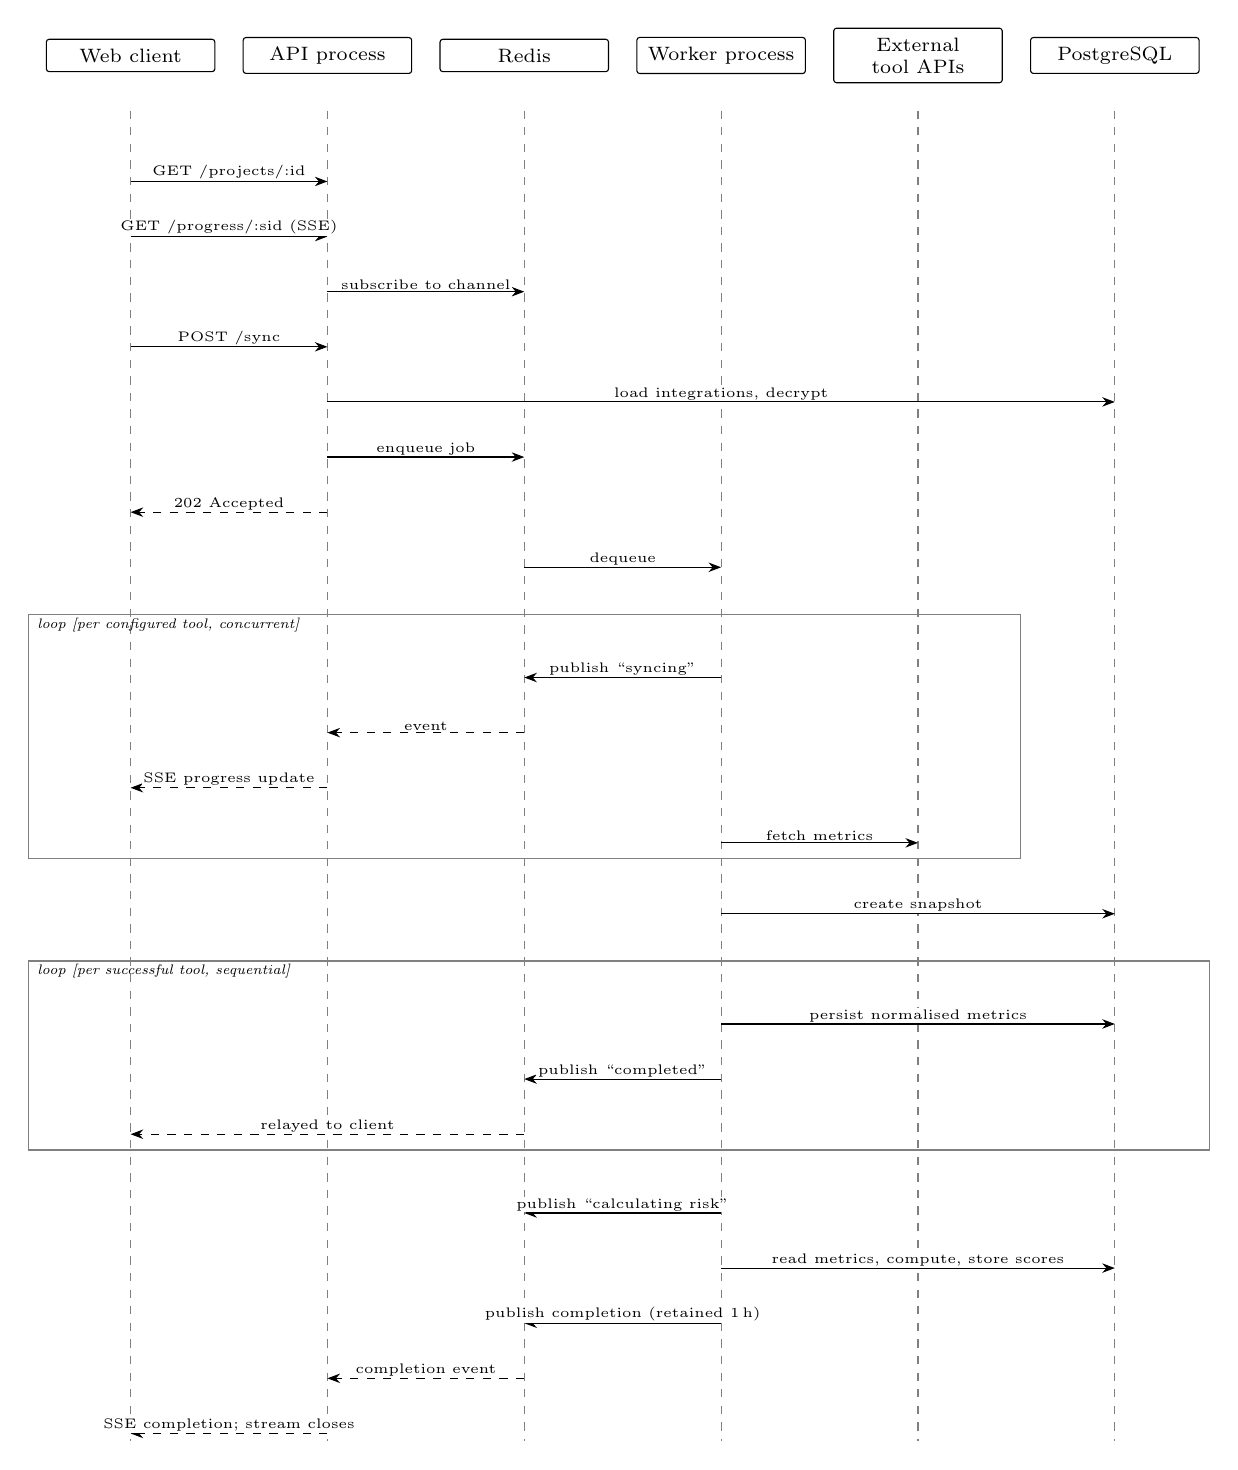
\begin{tikzpicture}[
  font=\scriptsize,
  head/.style={draw, rounded corners=1pt, align=center, text width=19mm,
               inner sep=1.2mm, font=\scriptsize},
  life/.style={dashed, gray},
  msg/.style={-{Stealth[length=1.6mm]}, thin},
  ret/.style={-{Stealth[length=1.6mm]}, thin, dashed},
  lbl/.style={font=\tiny, above, fill=white, inner sep=0.6pt},
  frame/.style={draw, thin, gray},
  ftag/.style={font=\tiny\itshape, anchor=north west, inner sep=1pt}
]

%% ---------- participants ----------
\node[head] (client) at (0mm,0mm)   {Web client};
\node[head] (api)    at (25mm,0mm)  {API process};
\node[head] (redis)  at (50mm,0mm)  {Redis};
\node[head] (worker) at (75mm,0mm)  {Worker process};
\node[head] (ext)    at (100mm,0mm) {External tool APIs};
\node[head] (db)     at (125mm,0mm) {PostgreSQL};

\foreach \x in {0,25,50,75,100,125}
  \draw[life] (\x mm,-7mm) -- (\x mm,-176mm);

%% ---------- setup ----------
\draw[msg] (0mm,-16mm)  -- node[lbl] {GET /projects/:id} (25mm,-16mm);
\draw[msg] (0mm,-23mm)  -- node[lbl] {GET /progress/:sid (SSE)} (25mm,-23mm);
\draw[msg] (25mm,-30mm) -- node[lbl] {subscribe to channel} (50mm,-30mm);
\draw[msg] (0mm,-37mm)  -- node[lbl] {POST /sync} (25mm,-37mm);
\draw[msg] (25mm,-44mm) -- node[lbl] {load integrations, decrypt} (125mm,-44mm);
\draw[msg] (25mm,-51mm) -- node[lbl] {enqueue job} (50mm,-51mm);
\draw[ret] (25mm,-58mm) -- node[lbl] {202 Accepted} (0mm,-58mm);
\draw[msg] (50mm,-65mm) -- node[lbl] {dequeue} (75mm,-65mm);

%% ---------- frame A: per tool, concurrent ----------
\draw[frame] (-13mm,-71mm) rectangle (113mm,-102mm);
\node[ftag] at (-13mm,-71mm) {~loop [per configured tool, concurrent]};
\draw[msg] (75mm,-79mm) -- node[lbl] {publish ``syncing''} (50mm,-79mm);
\draw[ret] (50mm,-86mm) -- node[lbl] {event} (25mm,-86mm);
\draw[ret] (25mm,-93mm) -- node[lbl] {SSE progress update} (0mm,-93mm);
\draw[msg] (75mm,-100mm) -- node[lbl] {fetch metrics} (100mm,-100mm);

%% ---------- snapshot ----------
\draw[msg] (75mm,-109mm) -- node[lbl] {create snapshot} (125mm,-109mm);

%% ---------- frame B: per successful tool ----------
\draw[frame] (-13mm,-115mm) rectangle (137mm,-139mm);
\node[ftag] at (-13mm,-115mm) {~loop [per successful tool, sequential]};
\draw[msg] (75mm,-123mm) -- node[lbl] {persist normalised metrics} (125mm,-123mm);
\draw[msg] (75mm,-130mm) -- node[lbl] {publish ``completed''} (50mm,-130mm);
\draw[ret] (50mm,-137mm) -- node[lbl] {relayed to client} (0mm,-137mm);

%% ---------- scoring and completion ----------
\draw[msg] (75mm,-147mm) -- node[lbl] {publish ``calculating risk''} (50mm,-147mm);
\draw[msg] (75mm,-154mm) -- node[lbl] {read metrics, compute, store scores}
(125mm,-154mm);
\draw[msg] (75mm,-161mm) -- node[lbl] {publish completion (retained 1\,h)}
(50mm,-161mm);
\draw[ret] (50mm,-168mm) -- node[lbl] {completion event} (25mm,-168mm);
\draw[ret] (25mm,-175mm) -- node[lbl] {SSE completion; stream closes} (0mm,-175mm);
\end{tikzpicture}
\caption{Synchronisation sequence. Solid arrows are requests and commands; dashed
arrows are responses and relayed events. Progress reaches the browser only by
being published to Redis and forwarded by the API process, because the worker
holds no client connection.}
\label{fig:sync-sequence}
\end{figure}

\paragraph{Ordering of fetch and persistence.}
The two loop fragments differ deliberately. Fetching is performed concurrently
across the configured tools, bounded by a concurrency limit, because the four
external APIs are independent and the elapsed time of a synchronisation is
dominated by network latency. Persistence is performed sequentially afterwards,
because every tool's output must attach to the same snapshot row. The snapshot is
created once, after at least one fetch has succeeded, and each tool's metrics are
then written against it. Creating the snapshot before the persistence loop rather
than lazily within it ensures that a failure part-way through cannot leave one
synchronisation's data split across two snapshot rows.

\paragraph{Partial completion.}
A tool that fails at either stage emits a failure event and is recorded in the
job's failed list, but does not abort the run (FR-19, NFR-10). The completion
event therefore carries three possible outcomes which are success, partial, or failed, 
derived from which tools succeeded, and additionally downgraded from success to partial 
if scoring itself failed, so that a run which collected data but
produced no usable score is not reported to the user as wholly successful.

\paragraph{Reconnection.}
The completion event is not only published but also retained in Redis for one
hour. When a client opens a progress stream, the API first checks for a retained
completion for that session and, if one exists, delivers it immediately and
closes the stream. This is what allows a user to reload the page or navigate away
during a long synchronisation and still receive its outcome on return (FR-17),
rather than subscribing to a channel on which nothing further will ever be
published.


\subsection{Application Programming Interface}
\label{subsec:api-surface}

The server exposes 54 HTTP endpoints beneath the version prefix
\texttt{/api/v1}, which is omitted from the paths listed in
\Cref{tab:api-surface}. The interface follows REST conventions in resource
naming and method semantics, with one deliberate exception: the progress endpoint
is a Server-Sent Events stream rather than a request-response resource, because
the client must receive an unbounded series of events for a single logical
operation.

\paragraph{Conventions.}
Authentication is carried by an \texttt{httpOnly} session cookie rather than a
bearer token. This suits a single-page client served from the same origin as the
API. The browser automatically attaches the cookie, including on the
\texttt{EventSource} connection used for progress streaming, which cannot carry
custom headers. Errors return a uniform \texttt{\{ message \}} body with a status
code distinguishing the cause. The status codes are 400 for malformed input, 401 for an absent or
expired session, 403 for an authenticated caller lacking rights to the resource,
404 for a resource outside the caller's company (so that cross-tenant probing
cannot distinguish "forbidden" from "nonexistent"), 409 for a conflicting state,
and 503 where an optional external capability is unavailable. Successful
mutations return 200 or 201, except synchronisation, which returns 202 to signal
that work has been accepted but not performed.

Within each router, literal path segments are registered before parameterised
ones --- \texttt{/projects/health} before \texttt{/projects/:id},
\texttt{/actions/search} before \texttt{/actions/:id} --- so that a literal
segment is not captured as an identifier by a more general route declared
earlier.

\begin{longtable}{
  >{\raggedright\arraybackslash}p{0.09\textwidth}
  >{\ttfamily\scriptsize\raggedright\arraybackslash}p{0.29\textwidth}
  >{\raggedright\arraybackslash}p{0.30\textwidth}
  >{\raggedright\arraybackslash}p{0.18\textwidth}
}
\caption{Endpoint inventory, excluding the \texttt{/api/v1} prefix}
\label{tab:api-surface}\\
\toprule
\textbf{Method} & \textbf{\normalsize\rmfamily Path} & \textbf{Purpose} &
\textbf{Auth required} \\
\midrule
\endfirsthead
\toprule
\textbf{Method} & \textbf{\normalsize\rmfamily Path} & \textbf{Purpose} &
\textbf{Auth required} \\
\midrule
\endhead
\bottomrule
\endlastfoot
\multicolumn{4}{l}{\textit{Service health}} \\
GET & /health & Service and dependency status & None \\
\addlinespace
\multicolumn{4}{l}{\textit{Authentication and account lifecycle}} \\
POST & /auth/send-verification-code & Email a signup verification code & None \\
POST & /auth/verify-email-code & Confirm a verification code & None \\
POST & /auth/register & Create a company and administrator, or join by invitation &
None \\
POST & /auth/login & Authenticate and open a session & None \\
POST & /auth/logout & Revoke the current session & None \\
GET & /auth/me & Resolve the authenticated user & Session \\
POST & /auth/forgot-password & Email a password reset link & None \\
POST & /auth/reset-password & Consume a reset token and revoke all sessions & None \\
GET & /auth/invite/:token & Inspect an invitation without consuming it & None \\
POST & /auth/accept-invite & Join a project as an existing user & Session \\
\addlinespace
\multicolumn{4}{l}{\textit{Workspaces and repository import}} \\
GET & /workspaces & List the company's workspaces & Session \\
POST & /workspaces & Create a workspace and import repositories & Session,
administrator \\
POST & /workspaces/preview-repos & List repositories reachable with a token, storing
nothing & Session, administrator \\
GET & /workspaces/:workspaceId/repos & List repositories, flagging those already
imported & Session, administrator \\
POST & /workspaces/:workspaceId/projects & Import further repositories as projects &
Session, administrator \\
\addlinespace
\multicolumn{4}{l}{\textit{Projects, health and configuration}} \\
GET & /projects & List accessible projects with latest scores & Session \\
GET & /projects/health & Dashboard feed: every accessible project with score history
& Session \\
GET & /projects/:id & Project detail, integrations and members & Session \\
GET & /projects/:projectId/health & Health history for one project & Session \\
GET & /projects/:projectId/snapshots /:snapshotId/score-breakdown /:scoreType &
Per-metric breakdown of one score & Session \\
PATCH & /projects/:projectId/integrations & Create or update a tool integration &
Session, administrator \\
PATCH & /projects/:projectId/tracked & Toggle portfolio tracking & Session,
administrator \\
POST & /projects/:projectId/invites & Invite a member by email & Session,
administrator \\
DELETE & /projects/:projectId/members /:userId & Remove a member & Session,
administrator \\
GET & /projects/:projectId/integrations /:toolName/token & Reveal the effective
credential & Session, administrator \\
\addlinespace
\multicolumn{4}{l}{\textit{Synchronisation}} \\
POST & /sync & Enqueue a synchronisation job & Session, project access \\
GET & /sync/:jobId & Inspect job state & Session \\
GET & /progress/:sessionId & Server-Sent Events progress stream & Session \\
\addlinespace
\multicolumn{4}{l}{\textit{Surveys, administrative}} \\
GET & /surveys & List surveys across projects & Requester-role header \\
GET & /surveys/:surveyId & Survey detail, responses and analysis & Requester-role
header \\
PATCH & /surveys/:surveyId/questions & Edit questions before dispatch &
Requester-role header \\
PATCH & /surveys/:surveyId/complete & Close and queue analysis & Requester-role
header \\
POST & /surveys/:surveyId/close & Close an active survey & Requester-role header \\
POST & /surveys/:surveyId/remind & Rebroadcast the link & Requester-role header \\
PATCH & /surveys/:surveyId/lifecycle & Pause, resume, retry or cancel &
Requester-role header \\
\addlinespace
\multicolumn{4}{l}{\textit{Surveys, project-scoped}} \\
POST & /projects/:projectId/surveys /generate-questions & Generate and score candidate
questions & Requester-role header \\
POST & /projects/:projectId/surveys /send-now & Create and dispatch immediately &
Requester-role header \\
POST & /projects/:projectId/surveys & Create and dispatch with supplied questions &
Requester-role header \\
GET & /projects/:projectId/surveys & List a project's surveys & Requester-role header
\\
GET & /projects/:projectId/surveys/quota & Remaining manual dispatches this month &
Requester-role header \\
GET & /projects/:projectId/surveys /schedule & Current month's scheduled pulse &
Requester-role header \\
GET & /projects/:projectId/pending-survey & Whether the project is flagged as due &
Requester-role header \\
\addlinespace
\multicolumn{4}{l}{\textit{Surveys, public respondent interface}} \\
GET & /public/surveys/:token & Retrieve the form behind an anonymous link & Token,
rate-limited \\
POST & /public/surveys/:token/responses & Submit an anonymous response & Token,
rate-limited \\
\addlinespace
\multicolumn{4}{l}{\textit{Management actions}} \\
POST & /actions & Record an action & Session \\
GET & /actions & List actions, scoped by role & Session \\
GET & /actions/search & Keyword or semantic search & Session \\
GET & /actions/effectiveness-review & Actions awaiting the author's review & Session
\\
GET & /actions/:id & Retrieve one action & Session \\
PUT & /actions/:id & Amend an action & Session \\
DELETE & /actions/:id & Delete an action & Session \\
PUT & /actions/:id/effectiveness & Rate effectiveness & Session, author only \\
PUT & /actions/:id/review-schedule & Defer the review & Session, author only \\
\end{longtable}

\paragraph{Tenancy scoping.}
Every endpoint marked \emph{Session} resolves the caller's company from the
session and restricts its query to that company. Project-scoped endpoints apply a
second check: an administrator may reach any project within their company, while
a member must additionally hold a membership record for the specific project. The
score-breakdown endpoint applies a third, because snapshot identifiers are
sequential across all projects and would otherwise be enumerable. It confirms
that the named snapshot belongs to the named project before serving it.

\paragraph{The public respondent interface.}
Two endpoints are reachable without a session, by design. A survey respondent is
not a user of the system and holds no account. Authorisation is carried instead
by the encrypted link token, which names the survey, its distribution cycle and
its deadline, and is sealed such that altering any of those fails decoding.
Because these endpoints are the system's only unauthenticated write surface, they
carry request rate limits, sixty form retrievals and ten submissions per
fifteen-minute window as defence in depth behind the token's own entropy.



\subsection{Design Calculations}
\label{subsec:design-calculations}

Two constraints established in \Cref{subsec:constraints} required
quantitative verification rather than assertion, the system had to operate
entirely within free service tiers (C-03), and it had to respect the rate limits
published by external providers (NFR-16). The estimates below were derived from
the connector metric schemas and the configured synchronisation cadence, and
determine whether the chosen parameters actually satisfy those constraints.

\paragraph{Storage per snapshot.}
Each synchronisation writes one \texttt{projectsnapshot} row, up to four metric
rows and one \texttt{riskscore} row. The metric payloads dominate. Their size was
estimated by counting the leaf fields of each connector's response type and
allowing approximately 38 bytes per field for the key string, value and
\texttt{jsonb} entry overhead, plus the contribution of the variable-length
arrays.

\begin{longtable}{
  >{\raggedright\arraybackslash}p{0.30\textwidth}
  >{\raggedright\arraybackslash}p{0.38\textwidth}
  >{\raggedright\arraybackslash}p{0.16\textwidth}
}
\caption{Estimated storage per snapshot}
\label{tab:storage-per-snapshot}\\
\toprule
\textbf{Component} & \textbf{Basis} & \textbf{Estimate} \\
\midrule
\endfirsthead
\toprule
\textbf{Component} & \textbf{Basis} & \textbf{Estimate} \\
\midrule
\endhead
\bottomrule
\endlastfoot
versioncontrolmetrics & 31 scalar fields, plus one entry per top-level directory
touched (assumed 15) & 2.3 kB \\
projectmanagementmetrics & 25 scalar fields, plus a sprint trend capped at 10 entries
& 1.5 kB \\
codequalitymetrics & 21 scalar fields, plus hotspot files capped at 5 entries & 1.2
kB \\
cicdmetrics & 10 scalar fields & 0.4 kB \\
projectsnapshot, riskscore and row overhead & Fixed-width columns & 0.3 kB \\
\midrule
\textbf{Total per snapshot} & & \textbf{$\approx$ 5.7 kB} \\
\end{longtable}

\paragraph{Storage growth.}
With the default schedule of one synchronisation per project per day, a project
accumulates 365 snapshots per year, or approximately 2.1\,MB. Allowing roughly
thirty per cent for indexes gives 2.7\,MB per project-year for scheduled
synchronisation alone. Manual synchronisation adds to this in direct proportion.
A team synchronising once more per working day approximately doubles the figure,
to about 5.4\,MB per project-year.

\begin{longtable}{
  >{\raggedright\arraybackslash}p{0.26\textwidth}
  >{\raggedright\arraybackslash}p{0.20\textwidth}
  >{\raggedright\arraybackslash}p{0.20\textwidth}
  >{\raggedright\arraybackslash}p{0.18\textwidth}
}
\caption{Projected database growth for a 25-project portfolio}
\label{tab:storage-growth}\\
\toprule
\textbf{Usage} & \textbf{Per project-year} & \textbf{25 projects, 3 years} &
\textbf{Free tier reached} \\
\midrule
\endfirsthead
\toprule
\textbf{Usage} & \textbf{Per project-year} & \textbf{25 projects, 3 years} &
\textbf{Free tier reached} \\
\midrule
\endhead
\bottomrule
\endlastfoot
Scheduled only & 2.7 MB & 203 MB & $\approx$ 7 years \\
Scheduled plus daily manual & 5.4 MB & 405 MB & $\approx$ 3.7 years \\
\end{longtable}

This is the least comfortable of the estimates. The managed database's free tier
provides 500\,MB, so a portfolio of twenty-five projects remains within it for
somewhere between four and seven years depending on how often users synchronise
manually --- adequate for the project's horizon, but not indefinitely. The
append-only snapshot model is what consumes the space, and it is also what makes
the remedy straightforward. Since each snapshot is self-contained, snapshots
older than a retention horizon can be deleted, or thinned to weekly resolution,
without affecting any other record. No such pruning is implemented, and it is
recorded as future work.

\paragraph{External request budget.}
The version-control connector dominates the request count, because it retrieves
the file list of every commit in a thirty-day window individually. For a
repository receiving approximately 200 commits per month the budget is as
follows.

\begin{longtable}{
  >{\raggedright\arraybackslash}p{0.40\textwidth}
  >{\raggedright\arraybackslash}p{0.44\textwidth}
}
\caption{Estimated version-control API requests per synchronisation}
\label{tab:api-budget}\\
\toprule
\textbf{Operation} & \textbf{Requests} \\
\midrule
\endfirsthead
\toprule
\textbf{Operation} & \textbf{Requests} \\
\midrule
\endhead
\bottomrule
\endlastfoot
Per-commit file detail (200 commits, concurrency 4) & $\approx$ 200 \\
Commit and closed-issue listing (paginated, 100 per page) & 3--4 \\
Pull requests with reviews, issues, branches (GraphQL) & 5--15 queries \\
Default branch, dependency alerts, secret-scanning alerts & 3--4 \\
\midrule
\textbf{Total per synchronisation} & \textbf{$\approx$ 210--260} \\
\end{longtable}

An authenticated personal access token permits 5{,}000 REST requests per hour,
which bounds the system at roughly nineteen to twenty-four synchronisations per
hour per credential. The scheduled fan-out spaces projects sharing a credential
ten minutes apart, producing at most six synchronisations per hour, or
approximately 1{,}500 requests which is around thirty per cent of the available
budget. The chosen spacing therefore satisfies NFR-16 with a headroom factor of
roughly three.

This holds up to eighteen projects per credential. Beyond that, the
180-minute cap on total spread causes further projects to be scheduled at the
same moment rather than spaced further apart, and the headroom narrows. A
workspace substantially larger than eighteen repositories would require the
spacing or cap to be reconsidered, which is why both are configurable rather than
fixed.

\paragraph{Worker throughput.}
Synchronisation duration is dominated by the same per-commit requests, issued at
a concurrency of four; together with the other three connectors, which run
concurrently with the version-control connector, a synchronisation is estimated
at one to three minutes for a repository of the size assumed above. The worker
processes two synchronisation jobs in parallel, so a twenty-five-project
scheduled run occupies approximately twenty-five to forty minutes of wall-clock
time. This fits comfortably within the 180-minute window over which the run is
spread, confirming that the queue is not the limiting factor but the deliberate
spacing is.

\paragraph{Cache and vector storage.}
The in-memory store holds three kinds of data, all small. Sessions are
approximately 200 bytes each with a one-day expiry. Queued jobs carry the
project's resolved integration credentials and are approximately 2--4\,kB each;
scheduled jobs retain their completed record for twenty-five hours so that their
deterministic identifiers stay reserved, giving roughly 100\,kB for a
twenty-five-project run. Retained completion events expire after one hour. The
total working set is well under one megabyte, against a free-tier allowance
measured in hundreds. Action embeddings occupy 768 four-byte components plus row
overhead, approximately 3.3\,kB per action, so even a corpus of a thousand
actions adds only some 3\,MB.

\paragraph{Conclusion.}
The calculations confirm that the design satisfies C-03 and NFR-16 with the
chosen parameters, and identify where each constraint would eventually bind: the
database free tier at roughly four to seven years of accumulated history for a
mid-sized portfolio, and the version-control rate limit at approximately eighteen
projects sharing a single credential. Both limits are addressed by configuration
rather than redesign which is a retention policy in the first case, and the already
configurable spacing and spread parameters in the second.




\subsection{Verification of the Design}
\label{subsec:design-verification}

Verification was applied at four levels, chosen so that each class of design risk
is checked by the cheapest mechanism capable of detecting it: static analysis for
type and contract errors, unit tests for the scoring model's arithmetic, live-API
scripts for connector behaviour against real providers, and end-to-end scripts
for the assembled pipeline.

\paragraph{Static verification.}
The entire codebase is written in a statically typed language with strict
compiler settings, and the connector and scoring layers are typed generically.
Each scoring strategy declares the metric object it consumes, so supplying a
strategy with the wrong metric type is a compile-time error rather than a runtime
one. Type checking and static analysis run on every change through continuous
integration (\Cref{sec:implementation}), which means a change that breaks a
contract between modules cannot reach the main branch.

\paragraph{Unit verification of the scoring model.}
The scoring model received the heaviest test coverage, because it is the
component whose failures are least visible. A connector that breaks produces an
obvious error, whereas a scoring defect produces a plausible but wrong number. Of
the 131 automated test cases, 83 target the risk engine.

\begin{longtable}{
  >{\raggedright\arraybackslash}p{0.34\textwidth}
  >{\raggedright\arraybackslash}p{0.12\textwidth}
  >{\raggedright\arraybackslash}p{0.38\textwidth}
}
\caption{Automated test coverage by area}
\label{tab:test-coverage}\\
\toprule
\textbf{Area} & \textbf{Cases} & \textbf{What is verified} \\
\midrule
\endfirsthead
\toprule
\textbf{Area} & \textbf{Cases} & \textbf{What is verified} \\
\midrule
\endhead
\bottomrule
\endlastfoot
Shared scoring functions & 26 & Normalisation at boundary values, weight
renormalisation when signals are absent, clamping of out-of-range inputs \\
Seven scoring strategies & 57 & Each dimension's best case scores 100 and worst case
0; weights match the documented rules; missing metrics are excluded rather than
treated as zero \\
Credential encryption & 4 & Round-trip correctness, distinct ciphertexts for
identical input, rejection of tampered ciphertext \\
Survey link tokens & 5 & Round-trip correctness, expiry detection, rejection of
tampered or malformed tokens \\
Survey question generation & 6 & Deduplication, quality gating, category diversity in
selection \\
Survey response validation & 6 & Answer-type conformance, rejection of answers
outside the survey \\
Scheduled synchronisation & 6 & Credential grouping, spacing and spread clamping,
deterministic job identifiers, continuation after one project fails \\
Timestamp handling & 7 & Correct interpretation of zone-naive and zone-aware values
\\
Concurrency helper and connector concurrency & 4 & Bounded parallelism, preservation
of result order \\
Semantic search, embeddings, reranking & 3 suites & Provider adapters and fallback
behaviour \\
\end{longtable}

The scoring tests are written against the published rules rather than against the
implementation, which is what allowed the restructuring from six categories to
seven to proceed with confidence. The tests encoded what each dimension was specified to produce, so a change that altered behaviour unintentionally
failed visibly.

\paragraph{Verification of connectors against live providers.}
Connector behaviour cannot be verified by unit tests alone, because the risk
being checked is precisely whether the provider's API behaves as the
implementation assumes. A separate script exists for each connector
(\texttt{test-github-metrics}, \texttt{test-jira},
\texttt{test-sonarqube-metrics}, \texttt{test-github-actions-metrics}), each of
which runs that connector against a real project and prints the complete
normalised metric object. These were used throughout development to confirm that
every field the scoring model expects is actually populated by real data, and to
identify the fields that are not. The unavailability of security alert counts
where scanning is disabled, and of coverage where no report is published, both
recorded as constraint C-05, were discovered this way rather than anticipated.

\paragraph{End-to-end verification of the pipeline.}
Two scripts verify the assembled system. \texttt{test-risk-scores} runs all four
connectors against a single real project and produces all seven scores,
exercising the complete path from provider APIs through normalisation and
persistence to the scoring engine which is the same path
\Cref{fig:connector-scoring} describes. A second script performs a smoke test of
the deployed stack. It confirms the API's health endpoint reports its
dependencies as reachable, confirms database connectivity, enqueues a
synchronisation job, and polls its status, thereby exercising the queue and
worker boundary that unit tests cannot reach.

\paragraph{Requirement traceability.}
\Cref{tab:verification-traceability} maps the requirements whose satisfaction
depends on design decisions rather than on straightforward implementation to the
verification that covers each.

\begin{longtable}{
  >{\raggedright\arraybackslash}p{0.14\textwidth}
  >{\raggedright\arraybackslash}p{0.36\textwidth}
  >{\raggedright\arraybackslash}p{0.34\textwidth}
}
\caption{Verification of design-critical requirements}
\label{tab:verification-traceability}\\
\toprule
\textbf{Requirement} & \textbf{Property to be verified} & \textbf{Verified by} \\
\midrule
\endfirsthead
\toprule
\textbf{Requirement} & \textbf{Property to be verified} & \textbf{Verified by} \\
\midrule
\endhead
\bottomrule
\endlastfoot
FR-22 & Scores computed from partial data, absent weights redistributed & Unit tests
on the shared weighting function and on each strategy \\
FR-19, NFR-10 & One tool failing does not abort a synchronisation & Scheduled-sync
processor tests; observed during live connector runs \\
NFR-12 & Repeated schedule triggers do not duplicate work & Scheduled-sync processor
tests on deterministic job identifiers \\
NFR-16 & External rate limits respected & Design calculation
(\Cref{subsec:design-calculations}); concurrency tests \\
NFR-01 & Credentials encrypted at rest & Encryption round-trip and tamper-rejection
tests \\
NFR-06 & Survey links tamper-evident & Token tamper-rejection tests \\
NFR-15 & Bounded concurrency on external calls & Concurrency helper tests \\
O-07, NFR-21 & New providers addable without changing scoring & Demonstrated
structurally by the placeholder connectors \\
\end{longtable}

\paragraph{Limitations of the verification performed.}
Three limitations should be stated. First, no automated integration tests execute
against a live database or queue; the boundary between the application and its
infrastructure is covered only by the manual test script. Second, the
connector verification scripts are observational rather than assertive. They
print their output for inspection rather than asserting expected values, which is
appropriate for data whose correct value changes with the repository but means
they cannot run unattended in continuous integration. Third, the calibration
constants in the scoring model are verified for internal consistency but not for
external validity. The tests confirm that a metric at its defined best scores
100, not that the threshold defining "best" is the right one. That remains open
work requiring real project outcomes to calibrate against.




\subsection{Design Refinements During Implementation}
\label{subsec:design-refinement}

The design described in this chapter is not the design the project began with.
Several structures were revised once implementation exposed problems that were
not visible on paper, and the schema migration history which includes seventeen migrations,
each recording its own rationale is the record of that revision.
\Cref{tab:refinements} summarises the changes that altered the design rather than
merely extending it.

\begin{longtable}{
  >{\raggedright\arraybackslash}p{0.26\textwidth}
  >{\raggedright\arraybackslash}p{0.28\textwidth}
  >{\raggedright\arraybackslash}p{0.30\textwidth}
}
\caption{Design refinements made during implementation}
\label{tab:refinements}\\
\toprule
\textbf{Change} & \textbf{Problem it addressed} & \textbf{Effect on the design} \\
\midrule
\endfirsthead
\toprule
\textbf{Change} & \textbf{Problem it addressed} & \textbf{Effect on the design} \\
\midrule
\endhead
\bottomrule
\endlastfoot
Per-tool credential columns on \texttt{project} replaced by a generic integration
table with a \texttt{jsonb} configuration & Twelve tool-specific columns had
accumulated; each new tool required further columns and a migration & Adding a tool
became a data change rather than a schema change \\
\addlinespace
Metric tables collapsed from one column per metric to a single \texttt{jsonb} column
& Every metric a connector gained required a migration, and the connector outputs are
nested rather than flat & Connector coverage could expand freely; the scoring layer
reads fields by name and tolerates absence \\
\addlinespace
Access tokens moved from individual projects onto the owning workspace & The same
credential was duplicated across every project imported from one organisation,
multiplying the cost of rotation & One credential per workspace, resolved at
synchronisation time \\
\addlinespace
Scoring model restructured from six risk categories to seven health dimensions & The
original categories conflated concerns the available metrics could distinguish, and
were oriented so that a lower score was better & Scores became uniformly
higher-is-better; columns were dropped rather than renamed \\
\addlinespace
Overall score changed from computed-on-read to persisted at synchronisation & The
aggregate was recomputed on every dashboard request and could not be indexed or
compared historically & One stored value per snapshot, computed by the same
null-aware mechanism as its components \\
\addlinespace
Timestamp columns converted from zone-naive to zone-aware & Values written as UTC
lost their offset on storage and were reinterpreted as local time by every client &
Chart labels and elapsed-time displays became correct regardless of the reader's
locale \\
\addlinespace
Embedding records keyed by model version & Changing embedding provider would
otherwise have required a destructive rewrite of every stored vector & A new
provider's vectors coexist with the old while backfill proceeds \\
\addlinespace
Credential encryption applied with a version-tagged ciphertext prefix & Introducing
encryption would otherwise have required backfilling every existing row before
deployment & Existing plaintext values remain readable and encrypt themselves when
next written \\
\addlinespace
Snapshot creation moved ahead of the per-tool persistence loop & A tool failing
part-way through persistence could leave one synchronisation's data split across two
snapshot rows & One snapshot per run, guaranteed structurally \\
\addlinespace
Superseded subsystems deleted rather than retained & A survey-score blending
subsystem, a per-member role column and an unused identifier column had stopped being
referenced & Dead structure removed rather than carried forward \\
\end{longtable}

Some of these are worth discussing, because each illustrates a different kind of
lesson.

\paragraph{Generalising structures that were shaped around specific tools.}
The first three entries share a cause. The system was built tool by tool, and
each new tool was initially accommodated by extending the schema to describe it such as
columns named for Jira's fields, then SonarQube's, then GitHub's. This works
until the third tool, at which point the cost of each addition becomes visible
and the structure's real shape which is a set of tools, each with a configuration,
becomes obvious. Replacing the specific columns with a generic integration table,
and the per-metric columns with a document per tool, is what makes the
extensibility claimed in \Cref{subsec:connector-scoring-structure} genuine. It is
worth being candid that this generality was arrived at by refactoring rather than
foreseen. The connector interface was designed for extension from the start, but
the persistence layer beneath it was not, and had to catch up.

\paragraph{Restructuring rather than renaming the scoring model.}
When the scoring model was revised from six categories to seven, the affected
columns were dropped and recreated rather than renamed, even where an obvious
correspondence existed such as the former delivery score and the new planning and
execution score. The reason is recorded in the migration itself. 
The old values were produced by a retired formula oriented so that a lower score
indicated better health, while the new model is oriented the opposite way.
Carrying the values forward under a new name would have produced a column whose
historical rows meant the inverse of its recent ones, which is worse than having
no history at all. Accepting the loss of prior data was the correct trade.


% \section{Application of Tools}
% \label{sec:tools}
% \guidance{Justify the selection of the important tools and technologies and
% state their relevant limitations.}


\section{Application of Tools}
\label{sec:tools}

The technology selections below were governed by three constraints established in
\Cref{subsec:constraints}. First, zero budget, so every service had to offer a
usable free tier (C-03); second, a five-person part-time team, so unfamiliar technology
carried a real cost (C-01, C-02); and third, no access to the partner's infrastructure,
so nothing could assume an agent or hosted runner inside their environment
(C-07). Each selection is justified against those constraints and its limitations
stated, including several that only became apparent in use.

\subsection{Language and Runtime}
\label{subsec:tool-runtime}

The server and client are both written in TypeScript on Node.js~20. A single
language across the API, the worker and the browser client meant that five
 developers moved between layers without a context switch, and more
substantively, that the contract between the connector layer and the scoring
layer is enforced by the compiler. Each scoring strategy declares the metric
object it consumes, so supplying a strategy with the wrong metric shape fails at
build time rather than producing a silently wrong number. Node's ecosystem also
provided official SDKs for the version-control provider, which removed a
substantial amount of pagination and authentication work.

\subsection{Server Framework and Integration SDKs}
\label{subsec:tool-server}

Express was chosen for the API for two reasons. Its middleware model matched the
cross-cutting concerns the system needed. Session resolution, tenancy scoping,
security headers, rate limiting, each of which is applied once rather than
per handler. And because Express exposes the raw response object, the
Server-Sent Events endpoint could be implemented directly, holding a connection
open and writing events as they arrive, without fighting an abstraction designed
around request-response.

Version-control access uses the provider's official SDK with its throttling and
retry plugins. The throttling plugin reads rate-limit information from the headers
of responses already in flight, which replaced an earlier approach in this codebase
that issued a separate rate-limit query before each guarded call which roughly
doubles the request count while not actually throttling, since concurrent callers
each observed the limit independently and each waited in parallel.


\subsection{Data Persistence}
\label{subsec:tool-database}

PostgreSQL was selected for a workload that is genuinely relational at its core. Companies own projects and projects own snapshots, but each connector returns a different nested metric document. PostgreSQL serves both. Conventional columns and foreign keys for the entity structure, and \texttt{jsonb} for the metric payloads. It also, through the \texttt{pgvector} extension, stores the action embeddings, which avoided introducing a separate vector database, a significant saving under C-03. Supabase provides it as a managed service with a free tier, accessed over a REST interface that requires no connection pool, which suits a deployment that may be suspended and resumed.


\subsection{Queueing, Caching and Scheduling}
\label{subsec:tool-queue}

Redis serves three purposes with one dependency. It backs the job queues, carries
the publish/subscribe channels through which synchronisation progress reaches the
API process, and stores sessions. BullMQ supplies the queue semantics the design
required without bespoke work, retries with exponential backoff, job priorities so
scheduled work cannot crowd out a user waiting on a synchronisation, delayed jobs
for the credential-spacing described in \Cref{subsec:design-calculations},
deterministic job identifiers for idempotence, and repeatable schedulers for the
periodic synchronisation.

\paragraph{Limitations.}
Consolidating three responsibilities onto one dependency also consolidates the
failure. Because sessions live in Redis, an outage prevents users from logging in
as well as preventing any work from running. The system has no degraded mode for
this. BullMQ's repeatable schedulers persist in Redis rather than in code, so a
schedule registered by an earlier deployment continues firing until explicitly
removed, which is why the worker reconciles the configured schedule against
Redis on every start rather than simply registering it. Its priority convention
is also a trap: an unset priority is treated as the highest, so the scheduled
work is given an explicit positive value while interactive work is deliberately
left unset.

\subsection{Client Application}
\label{subsec:tool-client}

The client is a React single-page application built with Vite and styled with
Tailwind, using Recharts for the trend visualisations and React Router for
navigation. React's component model suits a dashboard built from repeated card
and chart structures, and Recharts is declarative in the same idiom, so chart
configuration lives alongside the data rather than in imperative lifecycle code.
Vite's development proxy forwards API calls to the backend, making them
same-origin during development so that session cookies work without a CORS
configuration that differs from production.


\subsection{External Intelligence and Notification Services}
\label{subsec:tool-external}

Survey question generation, question scoring and response analysis use Google's
Gemini models, which were selected because a single provider covers both text
generation and the embeddings required for semantic action search, and because
its free tier made both feasible under C-03. Embeddings are stored at 768
dimensions, the smallest of the provider's recommended sizes, to reduce
storage and similarity-search cost. Semantic search results are optionally
reranked by a hosted reranking service, which improves precision over raw cosine
similarity without hosting a reranking model. Transactional email is delivered
through an HTTP API rather than SMTP, avoiding connection management, and survey
links are broadcast to team channels through their respective bot APIs.

\paragraph{Limitations.}
The language model's output is not deterministic and not guaranteed
well-formed, so every response is parsed defensively, validated against an
expected shape, and `for generated questions, those are passed through a quality gate
before use. The free tier permits the provider to use submitted inputs for
product improvement, which constrains what may be sent and is discussed in
\Cref{sec:standards}. There is no service-level guarantee, and model versions are
deprecated on the provider's schedule rather than the project's; the client is
therefore isolated behind an interface with a stub implementation, so that the
system degrades rather than fails when the provider is unavailable or
unconfigured. The reranking service is likewise optional, falling back to
keyword search, but it adds latency to the search path and introduces a further
external processor of partner data. Email deliverability depends on sender
verification and bounces are not currently handled.

\subsection{Engineering and Delivery Tooling}
\label{subsec:tool-delivery}

Tests run under Vitest, which reuses the same transform pipeline as the build and
therefore required no separate TypeScript or module configuration. Static
analysis uses ESLint with the TypeScript plugin. Continuous integration runs on
GitHub Actions, where the repository already lives, with path filtering so that a
change touching only the client does not run the server checks. The server
components are containerised so that the local and deployed environments differ
only in configuration. The API and worker are deployed to a container platform
that runs long-lived processes, which is necessary because the worker must hold queue
connections and cannot be expressed as a request-triggered function, while the
client is served as static assets by a separate platform that proxies API
requests to the backend, so that browser requests are same-origin in production
as well as in development.

% \section{Implementation}
% \label{sec:implementation}
% \guidance{Describe how the key modules were implemented and the development
% process followed (repository, version control, code review, CI/CD).}


\section{Implementation}
\label{sec:implementation}

\subsection{Implementation of the Key Modules}
\label{subsec:module-implementation}

\paragraph{Connector layer.}
Each connector is a class satisfying the single-method interface described in
\Cref{subsec:connector-scoring-structure}, responsible for turning one provider's
API into the normalised metric object its category defines. The version-control
connector is the largest, and combines both of the provider's interfaces. REST
for resources that paginate simply, such as commits and closed issues, and
GraphQL for those where a single query can retrieve a nested structure that REST
would require many round trips to assemble such as pull requests together with their
reviews, review comments and discussion threads. Requests that must be issued per
item, most notably the file list of each commit, are dispatched through a shared
bounded-concurrency helper rather than all at once, which is what keeps a
synchronisation within the request budget calculated in
\Cref{subsec:design-calculations}.

Every connector observes one discipline consistently, i.e., a metric that cannot be
determined is reported as \texttt{null}, never as zero. The distinction matters
downstream, because the scoring layer excludes a null metric and redistributes
its weight, whereas a zero would be scored as the worst possible value. This is
why, for example, the security alert count is null for a repository with
scanning disabled rather than being reported as no alerts.

\paragraph{Risk engine.}
Each of the seven dimensions is implemented as a strategy class that declares its
inputs as a list of weighted signals. A signal pairs a weight with a
normalised score, produced by applying one of six shared normalisation functions
to the raw metric, e.g. a rating converted to a scale, a count divided by project
size, a value interpolated between good and bad reference points, a value capped
once a target is reached, or a value scored by proximity to an ideal midpoint.
The strategy then delegates to a shared routine that discards absent signals,
rescales the remaining weights to sum to one, and returns both the score and the
weights actually applied. Because that routine returns the effective weights
rather than the declared ones, the per-metric breakdown of FR-26 is available
without any separate bookkeeping.

Two dimensions (engineering process, and planning and execution) are
computed as two independently weighted sub-groups combined afterwards using the
same routine one level up, so that a project with no issue-tracker data falls
back to its other sub-group rather than being scored as though half its inputs
were failing.

\paragraph{Synchronisation pipeline and progress streaming.}
The worker's synchronisation processor orchestrates one run. It fetches from the
configured tools concurrently, creates the snapshot once at least one fetch has
succeeded, writes each tool's output against that snapshot sequentially, then
invokes scoring. Each stage publishes an event to a Redis channel named for the
client's session. The API process holds the browser connection and subscribes to
that channel, relaying each event over Server-Sent Events; the completion event
is additionally stored under a session key with a one-hour expiry, so a client
that reconnects after the run has finished is served the stored outcome
immediately instead of subscribing to a channel that will not speak again.

Failure is handled per tool rather than per run. A connector that throws is
recorded as failed, its failure is published, and the remaining tools proceed;
the run's reported outcome is derived from which tools succeeded, and is further
downgraded if scoring itself failed, so that a run which gathered data but
produced no usable score is not reported as fully successful.

\paragraph{Survey subsystem.}
The survey feature is implemented across three queues and an hourly scheduled
tick. The tick assigns each project a randomised send moment within the
configured monthly window, fixing it on the survey row so it is decided once
rather than re-rolled; generates questions a configured number of days before
that moment; and dispatches at the moment itself. Question generation is a
pipeline rather than a single call. Candidates are generated, near-duplicates are
removed by a token-similarity comparison before any further paid call is made,
the survivors are scored by the model across four quality dimensions, those below
a threshold are discarded, and the remainder are selected preferring category
diversity. Dispatch mints an encrypted link token, broadcasts it once to the
configured team channels, and emails eligible developers individually, skipping
those inside their cooldown or owed a turn on another project.

\paragraph{Semantic action search.}
Recording an action enqueues an embedding job, which claims the work atomically
through a database function so that a retried job cannot embed twice, requests a
vector from the embedding provider, and stores it against the action keyed by
model version. Search has two modes. A lexical mode that queries the database
directly, and a deep mode that retrieves candidates within the caller's scope and
reranks them through a hosted reranking service. The deep path degrades to the
lexical one whenever reranking is unconfigured or unavailable, so the feature has
no hard dependency on either external service.

\paragraph{Security-related implementation.}
Credential encryption is applied inside the data-access functions rather than at
the call sites, so that every module above that boundary handles plaintext and
none can persist an unencrypted value. Ciphertexts carry a version prefix, which
allowed encryption to be introduced without backfilling existing rows. Sessions
are opaque identifiers stored in Redis against the user record, held in the
browser as \texttt{httpOnly} cookies, and indexed by user so that a password
reset can revoke every session that user holds.

\subsection{Development Process}
\label{subsec:development-process}

\paragraph{Repository organisation.}
The project is held in a single Git repository containing two independently
installable packages, one for the server and one for the client, each with its
own dependency manifest, TypeScript configuration and lint configuration. Within
the server package, code is separated into \texttt{apps}, holding the two runnable
processes, and \texttt{libs}, holding the domain libraries both processes share which mirrors the separation drawn in \Cref{fig:architecture}. Path aliases allow shared
code to be imported by a stable name rather than by relative traversal.

\paragraph{Version control workflow.}
Development proceeded on feature branches merged into \texttt{main} through pull
requests, of which thirty-six were opened over the course of the project across
282 commits. Branches were named either for the change they carried
(e.g., \texttt{cicd-pipeline}, \texttt{feat-secret-encryption}) or for their author
together with the area worked on (e.g., \texttt{abdullah-score-update},
\texttt{arafat-survey}); the convention was not fixed at the outset and both
forms persist. Merges preserve the branch history rather than squashing it, so
individual commits remain attributable after integration. Alongside the pull
request flow, some integration occurred by merging \texttt{main} directly into a
working branch, which appears in the history as ordinary merge commits.

Commit messages follow a conventional prefixed form
(\texttt{feat(projects): \ldots}) in part of the history and a free-form
descriptive style elsewhere. The convention was adopted partway through the
project rather than established at its start, and was not enforced by tooling.

\paragraph{Division of work.}
Work was partitioned along the module boundaries described in
\Cref{sec:architecture} rather than arbitrarily. The connector layer, the scoring
engine, the worker processes, the survey subsystem and the client application
were each taken up by a principal author, with others contributing. This mapping
of people onto modules was possible precisely because the modules communicate
through narrow interfaces, a connector is written against one method
signature, a scoring strategy against one metric type, so concurrent work on
different subsystems rarely produced conflicting changes to the same files.


\paragraph{Continuous integration.}
Every pull request and every push to \texttt{main} triggers an automated
pipeline. It begins by determining which packages a change touches, so that a
change confined to the client does not run the server checks and vice versa. For
the server it installs dependencies reproducibly from the lockfile, type-checks,
lints, builds, and runs the test suites with coverage measurement; for the client
it installs, type-checks, lints and builds. A final aggregating job succeeds only
if every job that ran passed, treating a skipped job as acceptable but a failed
or cancelled one as fatal, which gives a single status check suitable for
protecting the \texttt{main} branch. Concurrency control cancels any superseded
run for the same branch, so that only the most recent commit is validated.

\paragraph{Code review.}
Changes were reviewed by another team member before merging. Review focused on
correctness of the domain logic and on consistency with the module boundaries
described in \Cref{sec:architecture}, with the automated pipeline handling type,
style and test conformance so that review attention was spent on design rather
than on mechanical defects.

\section{Deployment}
\label{sec:deployment}
\guidance{Describe how the system is deployed and operated: the target
environment and infrastructure, configuration and release process,
monitoring and backup, and who operates and maintains it. State the
computing resources the deployment consumes; their environmental impact is
assessed in \Cref{sec:sustainability}.}
% Chapter 5 -- Rubric: PO4 (investigation, experiment, synthesis of conclusions),
% PO3 (3.4 evaluation against requirements), PO5 (application of modern tools)
\chapter{Investigation and Evaluation}
\label{ch:evaluation}

This chapter reports the investigative work carried out on the built system.
\Cref{sec:investigation} presents four investigations using analytical
derivation, structured adversarial inspection, automated test execution and
measured configuration evidence as appropriate to the question.
\Cref{sec:performance} evaluates the delivered system against every objective
and every functional and non-functional requirement of \Cref{ch:requirements}.
\Cref{sec:deviations} analyses each point at which the delivered system departs
from its specification and states the revision made or the reason none was made.

Pulse is a development-focused project rather than a research contribution, so
the investigations are validations of the design decisions that carried the most
risk rather than controlled experiments testing scientific hypotheses. Each
investigation states the form of evidence it can support; source inspection is
not presented as runtime measurement, and an unmeasured quantity is left
unresolved. One investigation (INV-2) tests the anonymity guarantee
adversarially, from the position of the most privileged insider.

Requirement identifiers (O-, FR-, NFR-, C-, G-, SH-, EC-) are those established
in \Cref{ch:problem,ch:research,ch:requirements}, so every claim here is
traceable back to a stated requirement. Repository-derived evidence was obtained
by executing the project's own tooling and inspecting the implementation paths
discussed below. The commands are listed in \Cref{subsec:reproduction} so the
figures can be reproduced. Where a quantity was not measured, the text says so
rather than estimating it.

\section{Experimental Investigation}
\label{sec:investigation}

\subsection{Selection of Investigations}
\label{subsec:investigation-selection}

Four decisions were judged to warrant investigation. A decision qualified if it
met at least two of three tests: its failure would invalidate a stated project
objective; its correctness is not observable from the user interface; and no
established practice prescribed the answer, so the team had to derive one.

\begin{longtable}{
  >{\raggedright\arraybackslash}p{0.07\textwidth}
  >{\raggedright\arraybackslash}p{0.33\textwidth}
  >{\raggedright\arraybackslash}p{0.17\textwidth}
  >{\raggedright\arraybackslash}p{0.30\textwidth}
}
\caption{Investigations and the design decisions they validate}
\label{tab:investigations}\\
\toprule
\textbf{ID} & \textbf{Decision under investigation} & \textbf{Objective / requirement at risk} & \textbf{Consequence if the decision is wrong} \\
\midrule
\endfirsthead
\toprule
\textbf{ID} & \textbf{Decision under investigation} & \textbf{Objective / requirement at risk} & \textbf{Consequence if the decision is wrong} \\
\midrule
\endhead
\bottomrule
\endlastfoot
INV-1 & Treating an absent metric by excluding it and renormalising the remaining
weights, rather than imputing a value for it & O-02, O-03, FR-22 & Projects with
partial tool coverage are scored unfairly, making the cross-project comparison
that is the product's central claim invalid \\
\addlinespace
INV-2 & Enforcing respondent anonymity in the database schema rather than in
application logic & O-04, NFR-07, NFR-08 & Respondents can be re-identified,
candour collapses, and the stakeholder conflict recorded in
\Cref{ch:requirements} (leadership insight vs.\ developer privacy) is
unresolved \\
\addlinespace
INV-3 & Using AI-assisted reranking to recover semantically related actions that
lexical matching can miss, while retaining lexical search as an independent
retrieval path & O-05, FR-39, NFR-13 & Without reranking, relevant actions
expressed with different vocabulary may be missed; when the provider is
unavailable, ordinary lexical retrieval remains available but explicit deep
search does not \\
\addlinespace
INV-4 & Bounded connector concurrency plus time-staggered scheduling to stay
inside free-tier API quotas & O-06, NFR-15, NFR-16 & A scheduled portfolio run
exhausts a shared credential's quota and the trend history that gives the product
its value develops gaps \\
\end{longtable}

\subsection{INV-1: Treatment of Absent Metrics in the Scoring Model}
\label{subsec:inv1}

\paragraph{The decision under investigation.} \Cref{ch:requirements} records
that most real projects have only a subset of the four tool categories
configured, and FR-22 requires that a score be computed from whichever metrics
are actually available. The scoring model must therefore define what a dimension
score \emph{means} when some of its input signals do not exist. Three treatments
were considered:

\begin{itemize}
  \item \textbf{Zero-imputation.} An absent signal scores 0 and retains its full
  weight.
  \item \textbf{Mean-imputation.} An absent signal takes the mean of the signals
  that are present, or of the portfolio.
  \item \textbf{Renormalisation.} An absent signal is excluded and the weights of
  the remaining signals are rescaled to sum to one. This is the treatment
  implemented by the shared scoring utility used across all risk dimensions.
\end{itemize}

The question is whether the choice is material, and if so which treatment is
defensible.

\paragraph{Why zero-imputation was rejected.} The objection is arithmetic rather
than empirical, and it can be shown with a single worked example using the
implemented weight vector of the security dimension
(\Cref{tab:security-weights}).

\begin{table}[H]
\centering
\caption{Implemented weight vector of the security dimension}
\label{tab:security-weights}
\begin{tabular}{llr}
\toprule
\textbf{Signal} & \textbf{Source tool} & \textbf{Weight} \\
\midrule
\texttt{securityRating} & SonarQube & 0.25 \\
\texttt{vulnCountDensity} & SonarQube & 0.20 \\
\texttt{securityReviewRating} & SonarQube & 0.15 \\
\texttt{securityHotspotsDensity} & SonarQube & 0.15 \\
\texttt{dependencyUpdateLag} & version control & 0.15 \\
\texttt{securityRemediationEffort} & SonarQube & 0.10 \\
\bottomrule
\end{tabular}
\end{table}

Consider a project that has connected version control but not SonarQube --- an
ordinary situation, and exactly the case FR-22 exists to handle. Five of the six
signals are absent, carrying 0.85 of the total weight. Suppose the one available
signal, \texttt{dependencyUpdateLag}, scores 80.

\begin{itemize}
  \item Under \textbf{renormalisation}, the single present signal's weight is
  rescaled from 0.15 to 1.0, and the dimension scores \textbf{80}. The score
  says: \emph{on the evidence available, this project's security posture looks
  good.}
  \item Under \textbf{zero-imputation}, the absent signals contribute
  $0.85 \times 0 = 0$ and the score is $0.15 \times 80 = 12$. The dimension
  scores \textbf{12}.
\end{itemize}

The same project, with identical underlying security practices, scores 80 or 12
depending only on whether an administrator has pasted in a SonarQube token.
Zero-imputation makes an absent measurement arithmetically indistinguishable
from a measurement of the worst possible value, so a project that has simply not
connected a tool is scored as though its code quality were \emph{known} to be
the worst observable.

This is disqualifying on two grounds. It violates FR-22 directly. More
seriously, it would defeat objective O-02: across a portfolio, the dominant
signal in the scores would be how many tools each project had configured, so the
cross-project comparison that the product exists to provide would be measuring
the wrong thing entirely. The distortion is also systematically
one-directional --- every absent signal drags the score down, never up --- so it
would not average out across a portfolio.

\paragraph{Why mean-imputation was rejected.} Mean-imputation avoids that bias
and, on accuracy alone, is a reasonable alternative to renormalisation. It was
rejected on a different ground.

Imputing the \emph{portfolio} mean makes one project's score depend on the
current state of every other project: a project's displayed score would change
when an unrelated project synchronised, without anything about the first project
having changed. That breaks O-03 and FR-26 outright, because a score breakdown
could no longer be stated in terms of that project's own metrics --- the honest
breakdown would have to read ``and 0.85 of this score is an assumption borrowed
from other projects.''

Imputing the project's \emph{own} mean avoids that coupling, but substitutes a
different problem: it fabricates evidence. It asserts that the project's
unmeasured security posture resembles its measured dependency hygiene, which is
an assumption the system has no basis for and cannot show the user.

Renormalisation makes the weaker and more honest claim --- \emph{this is the
score on the evidence available} --- and keeps every score a pure function of
that project's own inputs, which is what makes the per-signal breakdown of FR-26
possible at all.

\paragraph{Verification.} The implemented behaviour is asserted by the scoring
unit-test suite, which runs in CI on every change:

\begin{itemize}
  \item \texttt{renormalizedWeightedScore} \emph{``excludes missing signals and
  renormalizes the remaining weights to sum to 1''} (line 68) --- the direct
  assertion of FR-22.
  \item \emph{``computes a plain weighted average when every signal is
  present''} (line 56) --- confirms renormalisation is a no-op when nothing is
  missing, so the treatment does not perturb fully-configured projects.
  \item \emph{``returns null when no signal is present''} (line 48) --- a
  dimension with no evidence at all yields no score rather than a misleading
  zero, which is the same principle applied at the boundary.
  \item \emph{``excludes a present signal whose weight is 0''} and \emph{``clamps
  the result even if an individual signal score is out of 0..100''} (lines 80,
  89).
\end{itemize}

Each of the eight risk strategies additionally has a dedicated automated test
suite covering its signal set, satisfying NFR-22.

\paragraph{Limitation.} Renormalisation removes the bias, but it cannot
manufacture the information the absent signal would have carried. A dimension
score computed from two signals is a weaker estimate than one computed from six,
and the interface presents both identically --- a manager comparing two projects
cannot see that one score rests on materially less evidence. Team health is most
exposed, having only four signals, so a single absent input removes a quarter of
the evidence. This is recorded as an acknowledged limitation in
\Cref{subsec:deviation-confidence} and carried to future work.

\subsection{INV-2: Adversarial Investigation of Respondent Anonymity}
\label{subsec:inv2}

\paragraph{Research question.} NFR-07 requires that a survey response not be
attributable to the individual who submitted it. The absence of an identity
column establishes that no \emph{direct} attribution exists; it does not
establish that no attribution is \emph{possible}. The question is what an
adversary with realistic access could actually infer.

\paragraph{Threat model.} The adversary is the \textbf{company administrator}:
an insider with full read access to the tenant's data, including direct database
access, who wishes to learn how a named developer answered. This is the correct
adversary to model, because it is precisely the party whose access developers
(SH-03) are being asked to trust, and it is the strongest adversary the system
can meaningfully defend against. Defending against a database-level insider is
what distinguishes a structural guarantee from a policy promise.

\paragraph{Method.} Each plausible linkage route was enumerated and traced
through the applied response and recipient schemas, token representation,
dispatch path and insight-generation path. A route was classed as
\textbf{closed} only where the inspected representation contained no join key or
identity-bearing value; otherwise it was classed as \textbf{open} or
\textbf{statistically possible}. The result therefore establishes properties of
the evaluated implementation, not the probability of successful
re-identification in a real organisation.

\paragraph{Results.} \Cref{tab:anonymity} records each route attempted and its
outcome.

\begin{longtable}{
  >{\raggedright\arraybackslash}p{0.05\textwidth}
  >{\raggedright\arraybackslash}p{0.30\textwidth}
  >{\raggedright\arraybackslash}p{0.53\textwidth}
}
\caption{Re-identification routes attempted and outcomes}
\label{tab:anonymity}\\
\toprule
\textbf{\#} & \textbf{Linkage route} & \textbf{Outcome} \\
\midrule
\endfirsthead
\toprule
\textbf{\#} & \textbf{Linkage route} & \textbf{Outcome} \\
\midrule
\endhead
\bottomrule
\endlastfoot
A1 & \textbf{Direct.} A respondent column, foreign key or nullable author field
on \texttt{survey\_response} & \textbf{Closed by schema.} The table holds
\texttt{id}, \texttt{survey\_id}, \texttt{submission\_key} (a client-generated
UUID), \texttt{submitted\_at} and \texttt{answers} (jsonb). There is no identity
column and no foreign key to \texttt{User} \\
\addlinespace
A2 & \textbf{Token.} Recovering an individual from the access token embedded in
the survey link & \textbf{Closed by design.} \texttt{SurveyTokenPayload} is
\texttt{\{ surveyId, cycleId, deadline \}} only. One token is minted per
\emph{cycle}, not per recipient, so the token is byte-identical for every
developer on the project and carries no per-person information \\
\addlinespace
A3 & \textbf{Recipient join.} Correlating \texttt{survey\_recipient} rows
against \texttt{survey\_response} rows & \textbf{Closed.}
\texttt{survey\_recipient} records that a send was attempted and its outcome
(\texttt{sent}/\texttt{skipped}/\texttt{failed}). The only column it shares with
\texttt{survey\_response} is \texttt{survey\_id}, which is common to every
respondent, so the join is one-to-many in both directions and yields no
pairing \\
\addlinespace
A4 & \textbf{Timing.} Ordering responses by \texttt{submitted\_at} and
correlating against delivery times or individual working patterns &
\textbf{Open, statistical.} \texttt{submitted\_at} is stored at full precision
and is not coarsened. Because the link is broadcast once per cycle rather than
staggered per person, delivery time carries no per-person signal; but an
administrator could still correlate submission time against a developer's own
commit or CI activity, which the platform itself records. Narrowing rather than
identification, and harder as cohort size grows \\
\addlinespace
A5 & \textbf{Small cohort.} Inferring authorship on a project with very few
eligible respondents & \textbf{Open, statistical.} With few eligible respondents
the set of possible authors is small. This is a property of team size rather
than of anything the system stores, and narrows rather than identifies \\
\addlinespace
A6 & \textbf{Content.} A respondent identifying themselves within a free-text
answer, or writing in a recognisable style & \textbf{Open, irreducible.} No
technical control can prevent a respondent from identifying themselves in their
own words \\
\end{longtable}

\paragraph{Analysis and conclusion.} Route A1 is \textbf{closed structurally}:
direct attribution cannot be added without changing the response schema. Routes
A2 and A3 are closed by the current application and data design, but not by the
response schema alone. A future code change could mint a different token per
recipient, and a future schema or dispatch change could introduce a joinable
identifier. The defensible claim is therefore narrower: the stored response has
no direct identity field, while the shared-token and non-joinable-recipient
properties were verified by inspection of the evaluated implementation.

Routes A4--A6 are \textbf{statistical rather than structural}: they concern what
could be inferred from context, not what the system stores. \textbf{Respondent
anonymity is therefore enforced wherever the system can enforce it} --- no
stored response carries a respondent identity, the survey link is identical for
every recipient, and delivery records cannot be joined to responses. The
remaining routes depend on timing, team size and what respondents choose to
write, and no survey system can close them technically.

\subsection{INV-3: Availability of AI-Assisted Action Search}
\label{subsec:inv3}

\paragraph{Research question.} The action-search subsystem contains an ordinary
PostgreSQL lexical path and an explicitly requested \texttt{mode=deep} path that
reranks candidates through Pinecone. Lexical matching is fast and
provider-independent, but can miss conceptually related actions and problems
when they use different words; AI-assisted reranking exists to recover that
semantic similarity. A separate asynchronous pipeline generates Gemini
embeddings for actions. NFR-13 requires optional external-service
unavailability to produce graceful degradation. Does a deep-search request fall
back to lexical search when the reranker is unavailable, and what evidence
supports that behaviour?

\paragraph{Method.} The action-search endpoint was traced through its
request-handling and search-service layers. The acceptance criterion for full
conformance with NFR-13 was fixed before judging the result: when deep mode is
requested and Pinecone is unavailable, the endpoint must return lexical results
successfully and identify the serving path as lexical in its response metadata.
The three action-search test suites were then executed to determine whether that
failover is asserted automatically. Their test cases were reviewed as well as
counted, because a passing suite is evidence only for the behaviours it actually
asserts.

\paragraph{Results.} All 11 tests in the three suites pass (11/11, 836\,ms).
They assert query sanitisation and action scoping, Gemini request construction
and provider-response classification, and Pinecone result mapping and
malformed-score rejection. They do \textbf{not} invoke \texttt{searchActions()}
while the provider is unavailable, and therefore do not test lexical failover.

Inspection shows that the two paths currently remain separate rather than
switching automatically. With deep mode absent, the service calls PostgreSQL
lexical search and reports lexical mode. With deep mode requested, an
unavailable reranker produces an availability exception that the request layer
maps to HTTP \textbf{503} rather than initiating lexical retrieval. The
search-mode response metadata is set only after the service returns
successfully. Exposing that metadata cross-origin makes successful path
selection observable, but does not create automatic failover.

One availability property does hold independently: the embedding write path is
asynchronous, so logging an action does not block on Gemini. The embedding
record moves through pending, processing, ready and failed states, while a
content hash prevents unchanged actions from being embedded repeatedly. These
properties protect action creation, but they do not change the HTTP 503
behaviour of a requested deep search.

\paragraph{Analysis and conclusion.} NFR-13 is \textbf{partially satisfied}.
Ordinary lexical search remains usable without either AI provider, so the action
log remains searchable during an outage. A user who explicitly requests deep
search, however, receives a 503 when Pinecone is unavailable, so the experience
does not yet meet the stated graceful-degradation criterion. Full conformance
requires catching \texttt{ActionRerankingUnavailableError}, executing the
lexical query, returning HTTP 200 with \texttt{x-action-search-mode: lexical},
and adding integration tests for both unconfigured and temporarily unavailable
provider cases.

The honest limitation is that this establishes path availability, not retrieval
quality. The investigation does \textbf{not} show that Pinecone reranking
returns more relevant results than lexical search. Establishing that would
require a labelled query corpus with relevance judgements fixed in advance,
measured by recall@5 and mean reciprocal rank against the lexical baseline. That
corpus does not exist: the action log accumulates from first use (C-06) and
there is no partner action history to draw on.

A second exposure is that survey question generation and survey insight
generation also have no non-AI substitute: an extended Gemini outage postpones a
survey cycle rather than serving a reduced version of it. This is recorded as
residual risk R2 in \Cref{subsec:planning}.

\subsection{INV-4: Rate-Limit Headroom of Portfolio Synchronisation}
\label{subsec:inv4}

\paragraph{Research question.} Constraint C-03 confines the system to free
service tiers, and \Cref{ch:requirements} records the resulting conflict between
the client's expectation of current data and the providers' published rate
limits. Scheduled synchronisation (FR-18) fans out across every configured
project, and all projects imported from one workspace share a single access
credential. How many projects can one credential carry before a scheduled run
exhausts its quota?

\paragraph{Method and measured parameters.} The governing parameters were read
from the shipped configuration and code rather than assumed
(\Cref{tab:sync-parameters}).

\begin{longtable}{
  >{\raggedright\arraybackslash}p{0.30\textwidth}
  >{\raggedright\arraybackslash}p{0.28\textwidth}
  >{\raggedright\arraybackslash}p{0.30\textwidth}
}
\caption{Measured throttling and scheduling parameters}
\label{tab:sync-parameters}\\
\toprule
\textbf{Parameter} & \textbf{Value} & \textbf{Source} \\
\midrule
\endfirsthead
\toprule
\textbf{Parameter} & \textbf{Value} & \textbf{Source} \\
\midrule
\endhead
\bottomrule
\endlastfoot
Per-project tool fetch concurrency & 4 & Worker configuration, confirmed by
inspection \\
\addlinespace
Concurrency primitive & Bounded worker pool, rejects non-positive integers &
Shared synchronisation utility, unit-tested \\
\addlinespace
Spacing between projects sharing one credential & 10\,min default (bounded
0--240) & Scheduling configuration, confirmed by inspection \\
\addlinespace
Maximum scheduling spread & 180\,min default (bounded 0--1440) & Scheduling
configuration, confirmed by inspection \\
\addlinespace
Schedule time zone & Configurable, default UTC & Scheduling configuration,
confirmed by inspection \\
\addlinespace
Schedule times & Comma-separated HH:MM, validated and range-checked &
Configuration parser and validation tests \\
\addlinespace
Idempotency of a retried tick & Deterministic job ID per project and slot &
Synchronisation service and scheduled-worker tests \\
\addlinespace
GitHub GraphQL rate-limit guard & Pre-flight check of remaining quota against a
threshold & Version-control connector inspection \\
\end{longtable}

The scheduler assigns project index $i$ the delay $\min(iS, W)$. Where $S$ is
positive, this provides $\lfloor W/S \rfloor + 1$ distinct launch positions,
including time zero and the maximum-delay position. With the defaults
($S = 10$ minutes, $W = 180$ minutes), there are therefore \textbf{19 distinct
positions}: 0, 10, \ldots, 180 minutes. Projects 1--19 can occupy distinct
scheduled positions; project 20 and every subsequent project in the same
credential bucket are also assigned minute 180 and begin to overlap at the
scheduling level.

This calculation bounds launch spacing, not the number of simultaneously running
syncs. Actual overlap also depends on each sync's wall-clock duration, BullMQ
worker concurrency and queue backlog. Likewise,
\texttt{TOOL\_FETCH\_CONCURRENCY = 4} caps connector work \emph{inside one
project sync}; it is not a bound of four concurrent project syncs and cannot by
itself establish compliance with a provider quota.

\paragraph{Results and limitation.} The derivation above is sound but
\textbf{incomplete in one input}: the number of API calls issued per connector
per project sync was not instrumented, so the ceiling cannot be expressed in
projects-per-credential against a provider's published quota. Reading it off the
source is unreliable because the GitHub connector paginates and issues both REST
and GraphQL calls whose count depends on repository size.

\paragraph{Analysis and conclusion.} Two narrower conclusions are supported.
First, staggering reduces the initial request burst for the first 19 projects in
a credential bucket, while the per-project worker pool bounds simultaneous
connector fetches within each sync. Neither fact proves that rate-limit failure
becomes merely a longer run; that claim requires the missing call-count,
duration and worker-concurrency measurements. Second, the deterministic job
identifier makes a retried scheduled tick a no-op (NFR-12), so retrying the same
slot does not duplicate that slot's request volume. The projects-per-credential
ceiling remains unknown and is recorded as residual risk R1 in
\Cref{subsec:planning}.

\subsection{Synthesis}
\label{subsec:synthesis}

The four investigations support four bounded conclusions about the built system.
The scoring model's treatment of missing data is \textbf{sound by
construction} --- the rejected alternative would have scored an otherwise
identical project 12 instead of 80 on the worked example of \Cref{subsec:inv1},
purely for having one tool unconfigured --- which is the basis for the
cross-project comparability claimed by O-02. \textbf{Respondent anonymity is
enforced}: survey responses contain no identity field, the per-cycle token
carries no per-person information, and delivery records cannot be joined to
responses; the residual routes are statistical inferences from context rather
than stored linkages. AI-assisted reranking addresses semantic relationships
that lexical matching can miss; ordinary lexical search remains available
without AI, while explicit deep search currently returns 503 when Pinecone is
unavailable, so NFR-13 is partially met. Scheduled synchronisation has verified
staggering and idempotency controls, but its projects-per-credential capacity
remains unquantified until runtime request counts and durations are measured.

Collectively, the investigations also validate the decision recorded in
\Cref{ch:requirements} to prefer a rule-based scoring model over a learned or
LLM-judged one: INV-1 was possible \emph{at all} only because the model is
deterministic and decomposable, and neither of the rejected alternatives could
have been audited this way.

\section{Performance Evaluation}
\label{sec:performance}

\subsection{Setup, Tooling and Acceptance Criteria}
\label{subsec:eval-setup}

Every change reaching the main branch is validated by an automated pipeline that
is a required status check under branch protection. The evaluation below
therefore describes a branch state that is, by construction, the state of every
merged change rather than a specially prepared build.

The pipeline applies a path filter (\texttt{dorny/paths-filter}) so that a
backend-only change does not run frontend jobs and vice versa, with a
\texttt{concurrency} group that cancels superseded runs,
\texttt{permissions: contents: read}, and a single aggregate \texttt{ci-ok} job
that treats a skipped one-sided job as a pass and any failure or cancellation as
a failure.

For the backend the pipeline runs, in order: strict TypeScript type checking,
ESLint, a production build, \texttt{test:coverage} (Vitest with V8 coverage),
and \texttt{test:actions} (three \texttt{node:test} suites). For the frontend it
runs type checking, linting and a production build with
\nolinkurl{VITE_API_BASE_URL=/api/v1} baked in.

\paragraph{A note on the coverage figure.} The test runner is configured to
instrument \textbf{every backend application and library source unit}, rather
than only units imported by a test. This is a deliberate methodological choice
and it makes the headline number look far worse than a default configuration
would. Default instrumentation reports the percentage of \emph{the code the
tests already reach}, which flatters a codebase by silently excluding exactly
the modules nobody has tested. Instrumenting every source unit means an untested
module appears as 0\,\% rather than as an absence. The figure below is therefore
a percentage \textbf{of the system}, not a percentage of the tested part of it,
and \textbf{it is not comparable with a default-configured figure from another
project.}

Four verification methods are used in the tables that follow, each requirement
being assigned the weakest method sufficient to establish it:

\begin{itemize}
  \item \textbf{T --- Test.} An automated test asserts the behaviour and runs in
  CI on every change.
  \item \textbf{D --- Demonstration.} The behaviour was exercised end-to-end
  against the running system and observed.
  \item \textbf{I --- Inspection.} The property is established by reading the
  schema, configuration or source, and is not observable at run time.
  \item \textbf{A --- Analysis.} The property is established by derivation or by
  one of the investigations in \Cref{sec:investigation}.
\end{itemize}

Statuses are \textbf{Met}, \textbf{Partial} (met in part, or met by a weaker
mechanism than specified), \textbf{Not met}, and \textbf{Unverified} (not
established by any of the four methods; no claim is made).

\subsection{Measured Results}
\label{subsec:measurements}

All figures below were obtained by running the commands listed in
\Cref{subsec:reproduction}.

\begin{longtable}{
  >{\raggedright\arraybackslash}p{0.42\textwidth}
  >{\raggedright\arraybackslash}p{0.48\textwidth}
}
\caption{Quantitative results}
\label{tab:measurements}\\
\toprule
\textbf{Measure} & \textbf{Result} \\
\midrule
\endfirsthead
\toprule
\textbf{Measure} & \textbf{Result} \\
\midrule
\endhead
\bottomrule
\endlastfoot
TypeScript strict type check (backend) & \textbf{Pass} (exit 0) \\
ESLint (backend) & \textbf{Pass} (exit 0) --- no blocking findings and 131
warnings, predominantly \texttt{@typescript-eslint/no-explicit-any} \\
Vitest suites & \textbf{20 files, 131 tests, 131 passed, 0 failed}, 3.15\,s \\
\texttt{node:test} action-search suites & \textbf{11 tests, 11 passed, 0
failed}, 836\,ms \\
Total automated tests & \textbf{142 across 23 test files} \\
Statement coverage (all-files instrumented) & 12.37\,\% (722 / 5,835) \\
Branch coverage & 12.34\,\% (489 / 3,961) \\
Function coverage & 9.75\,\% (99 / 1,015) \\
Line coverage & 12.93\,\% (685 / 5,295) \\
Frontend automated tests & \textbf{None} \\
\end{longtable}

\begin{longtable}{
  >{\raggedright\arraybackslash}p{0.30\textwidth}
  >{\raggedright\arraybackslash}p{0.14\textwidth}
  >{\raggedright\arraybackslash}p{0.44\textwidth}
}
\caption{Statement coverage by area, showing where testing effort was
concentrated}
\label{tab:coverage-by-area}\\
\toprule
\textbf{Area} & \textbf{Statement coverage} & \textbf{Interpretation} \\
\midrule
\endfirsthead
\toprule
\textbf{Area} & \textbf{Statement coverage} & \textbf{Interpretation} \\
\midrule
\endhead
\bottomrule
\endlastfoot
Security and token utilities & \textbf{91.66\,\%} & The cryptographic core is
the most heavily tested code in the system, appropriately \\
\addlinespace
Version-control throttling and retry utility & 69.56\,\% & Provider throttling
and retry behaviour \\
\addlinespace
Risk-engine subsystem & 52.38\,\% & The eight strategies and scoring arithmetic
are covered; the dispatcher and descriptive signal catalogue are untested \\
\addlinespace
Synchronisation utilities & 52.17\,\% & Bounded-concurrency behaviour is
covered; connector registration is untested \\
\addlinespace
\texttt{GithubActions} / \texttt{Github} connectors & 14.67\,\% / 12.79\,\% &
Exercised only incidentally \\
\addlinespace
\texttt{Jira}, \texttt{SonarQube}, \texttt{GitLab}, \texttt{Linear} connectors &
0\,\% & Not unit-tested; validated by demonstration against live APIs instead \\
\addlinespace
Queueing, notifications, embeddings, authentication and reranking & 0\,\% &
I/O-boundary modules, exercised through doubles or by demonstration \\
\end{longtable}

\paragraph{Interpretation.} The distribution is more informative than the
headline. Testing effort went where correctness is both critical and cheaply
assertable --- cryptography, scoring arithmetic, concurrency bounds --- and the
near-zero areas are overwhelmingly I/O boundaries against third-party services,
which unit tests can only assert against a double anyway. That is a defensible
allocation under constraint C-02 (no dedicated QA member). It is nonetheless a
real limitation, and it should be stated plainly rather than explained away:
\textbf{NFR-22 requires scoring rules to be documented and covered by automated
tests and that is satisfied, but the system as a whole rests on 142 tests and
has no frontend test at all.} A regression in the React application would be
caught only by type checking, linting and manual use.

\paragraph{Security review.} \Cref{ch:requirements} commits the project to
OWASP-aligned practice. The team reviewed the implementation manually against
the OWASP Top~10 --- authentication and session handling, access control,
injection, cryptographic storage of connector credentials, and rate limiting of
the unauthenticated survey endpoint. The codebase was additionally analysed with
SonarQube through Pulse's own SonarQube connector, so the platform's security
dimension was applied to its own repository. This is an internal review rather
than an independent third-party assessment.

\paragraph{Partner acceptance.} The system was not piloted against SSCL's own
GitHub, Jira or SonarCloud data. Evaluation used the team's own repositories and
tool accounts, which exercised every connector end to end without bringing
partner data into the development environment. The system was instead reviewed
with SSCL's Chief Technical Officer in five meetings, each held after a major
improvement (\Cref{subsec:multidisciplinary}).

\subsection{Evaluation Against Functional Requirements}
\label{subsec:eval-fr}

\begin{longtable}{
  >{\raggedright\arraybackslash}p{0.07\textwidth}
  >{\raggedright\arraybackslash}p{0.06\textwidth}
  >{\raggedright\arraybackslash}p{0.57\textwidth}
  >{\raggedright\arraybackslash}p{0.13\textwidth}
}
\caption{Verification of functional requirements}
\label{tab:fr-verification}\\
\toprule
\textbf{ID} & \textbf{M.} & \textbf{Evidence} & \textbf{Status} \\
\midrule
\endfirsthead
\toprule
\textbf{ID} & \textbf{M.} & \textbf{Evidence} & \textbf{Status} \\
\midrule
\endhead
\bottomrule
\endlastfoot
FR-01 & I, D & Registration creates a company and administrator account; a
one-time verification code is retained transiently and the account is created
only after verification & Met \\
FR-02 & T, I & Login service and persisted server-side session store & Met \\
FR-03 & I & Single-use reset token; the reset flow explicitly invalidates every
existing session belonging to the user & Met \\
FR-04 & I, D & Single-use invitation accepted during registration or by an
authenticated account & Met \\
FR-05 & T, I & Central authorisation service and requester-role resolution;
member access gated on project-membership records & Met \\
FR-06 & D & Administrator removes a \texttt{projectmember} row & Met \\
FR-07 & D & Workspace endpoint binds a workspace to its provider, organisation
identifier and access token & Met \\
FR-08 & D & Workspace interface lists reachable repositories through the
provider adapter before any persistence & Met \\
FR-09 & D & Selected repositories imported as \texttt{project} rows & Met \\
FR-10 & D & Subsequent import excludes already-imported repositories & Met \\
FR-11 & D & Per-project \texttt{projecttoolintegration} rows for PM, quality and
CI/CD; VCS credential inherited from workspace & Met \\
FR-12 & I, D & Credentials masked by default; reveal is a separate
administrator-restricted action & Met \\
FR-13 & D & \texttt{POST /sync} enqueues a job and returns job ID and stream key
immediately & Met \\
FR-14 & T, D & Implemented connectors cover VCS, issue tracking, code analysis
and CI/CD & Met \\
FR-15 & I & One \texttt{projectsnapshot} row per run; raw metrics as JSONB in
four per-domain tables keyed by \texttt{snapshot\_id}; no update path & Met \\
FR-16 & D & SSE over \texttt{/progress}; per-tool status rendered by
\texttt{SyncProgressBanner} & Met \\
FR-17 & I, D & Persistent event store replays missed progress events to a
reconnecting client & Met \\
FR-18 & T, I & Schedule queue is reconciled from configured times when the
worker starts; covered by scheduled-worker tests & Met \\
FR-19 & I & Synchronisation processing tracks unsuccessful tools, marks each
tool's outcome, persists successful results and reports the run as partial &
Met \\
FR-20 & T & Eight strategy classes, each with its own automated test suite &
Met \\
FR-21 & T & Overall score composed from dimension scores per snapshot;
\texttt{riskscore.overall\_score} & Met \\
FR-22 & T, A & Scoring tests assert that missing signals are excluded and
remaining weights are renormalised to sum to one; design rationale in
\Cref{subsec:inv1} & Met \\
FR-23 & I & \texttt{riskscore} rows keyed to \texttt{project\_snapshot\_id}
(unique) & Met \\
FR-24 & D & Portfolio dashboard lists accessible projects with overall score,
dimension scores and trend & Met \\
FR-25 & D & Per-project view with current score, trend and dimension history
(Recharts) & Met \\
FR-26 & D, I & Score-breakdown interface renders contributing signals, values,
weights and contributions from the signal catalogue & Met \\
FR-27 & I, D & Survey-question service generates from health scores, trend and
notable metric conditions & Met \\
FR-28 & T & Deterministic deduplication followed by a scoring prompt with a
configurable minimum score of 60 & Met \\
FR-29 & I, D & Questions editable while \texttt{draft}; editing rejected once
\texttt{sent\_at} is set & Met \\
FR-30 & T, I & Distribution processor assigns a randomised monthly send moment
per project within a configurable window, fixed once assigned & Met \\
FR-31 & D & On-demand dispatch available to an authorised user & Met (pending
confirmation) \\
FR-32 & I, D & One anonymous link per cycle, broadcast to configured channels and
emailed individually to eligible developers & Met \\
FR-33 & I & Cooldown enforced from \texttt{survey\_recipient} history against
\texttt{SURVEY\_MIN\_DAYS\_BETWEEN\_SURVEYS} (default 15, bounded 1--60);
skipped sends recorded with \texttt{skip\_reason: 'cooldown\_active'}. Fair
rotation between a developer's projects is unconfirmed & Partial \\
FR-34 & T & Automated token tests cover decoding, cycle validation and deadline
expiry & Met \\
FR-35 & I, D & Survey-insight service produces category scores, themes,
narrative summary and per-question summaries on close & Met \\
FR-36 & I, D & \texttt{project\_survey\_status.pending\_survey} raised when
configured thresholds are breached & Met \\
FR-37 & D & \texttt{actions} row carrying problem, reason, action taken, date
and affected \texttt{project\_ids} & Met \\
FR-38 & D & Per-project and company-wide listings, scoped by role & Met \\
FR-39 & T, A & Lexical search and optional Pinecone reranking are implemented.
Ordinary lexical retrieval remains available without AI, but a requested deep
search returns 503 rather than falling back when Pinecone is unavailable;
investigation INV-3 (\Cref{subsec:inv3}) & Partial \\
FR-40 & I, D & \texttt{next\_review\_at} with deferral presets; non-modal
\texttt{WeeklyReviewBanner} and \texttt{InlineRating} & Met \\
FR-41 & I & Author may modify or delete own actions; administrator may do so for
any action in the company (\texttt{logged\_by\_user\_id},
\texttt{company\_id} on \texttt{actions}) & Met \\
\end{longtable}

\subsection{Evaluation Against Non-Functional Requirements}
\label{subsec:eval-nfr}

\begin{longtable}{
  >{\raggedright\arraybackslash}p{0.08\textwidth}
  >{\raggedright\arraybackslash}p{0.06\textwidth}
  >{\raggedright\arraybackslash}p{0.56\textwidth}
  >{\raggedright\arraybackslash}p{0.13\textwidth}
}
\caption{Verification of non-functional requirements}
\label{tab:nfr-verification}\\
\toprule
\textbf{ID} & \textbf{M.} & \textbf{Evidence} & \textbf{Status} \\
\midrule
\endfirsthead
\toprule
\textbf{ID} & \textbf{M.} & \textbf{Evidence} & \textbf{Status} \\
\midrule
\endhead
\bottomrule
\endlastfoot
NFR-01 & T, I & Credential-security subsystem encrypts connector secrets at rest
with AES-256-GCM, a 12-byte random IV per record and a 16-byte authentication
tag; 92.59\,\% statement coverage & Met \\
NFR-02 & I & \texttt{bcryptjs} at 10 rounds, 8-character minimum enforced at
registration; no recovery path exists & Met \\
NFR-03 & I & Session ID in a cookie with \texttt{httpOnly: true},
\texttt{secure: env.nodeEnv === 'production'}, \texttt{sameSite: 'lax'};
revocable via \texttt{sessionStore.destroy} / \texttt{destroyAllForUser} &
Met \\
NFR-04 & I & Credentials masked except through the FR-12 reveal action;
credential used as a scheduling grouping key is reduced to a one-way hash first
& Met (pending confirmation) \\
NFR-05 & I & Request-rate limiting is applied to the public survey endpoint with
distinct limits for form retrieval and submission; this is the only
unauthenticated endpoint family & Met \\
NFR-06 & T & AES-256-GCM authentication tag makes modification of the embedded
\texttt{surveyId}, \texttt{cycleId} or \texttt{deadline} fail decode rather than
succeed with altered values; \texttt{decodeToken} returns \texttt{null} rather
than throwing & Met \\
NFR-07 & I, A & No identity column or user foreign key on
\texttt{survey\_response} (structural); the shared-token and
non-joinable-recipient properties were verified by inspection
(\Cref{subsec:inv2}) & Met \\
NFR-08 & I & Aggregate survey insight is generated only once the number of
responses reaches the configured minimum
(\texttt{SURVEY\_MIN\_ANONYMOUS\_RESPONSES}, default 5, floor 3); below it, no
insight is produced & Met \\
NFR-09 & I & No personal identifiers found in the AI payload construction:
inspection for author, assignee, login, email, issue-key and branch fields found
only aggregate scores, depersonalised conditions, the project name and
respondent count. \textbf{However, free-text survey answers are transmitted
verbatim and may contain names the system cannot strip} (gap G-03) & Partial \\
NFR-10 & I & A failing connector does not abort the remaining connectors; the
run is recorded as partial (\texttt{failedTools[]}) & Met \\
NFR-11 & I & BullMQ retry with increasing backoff on every queue & Met \\
NFR-12 & T & Deterministic job identifier per project and time slot makes a
repeated or retried tick a no-op & Met \\
NFR-13 & I, A & Lexical search remains available as the ordinary mode, but it is
not used as failover: an unconfigured or failed Pinecone deep search returns
HTTP 503. The current tests do not assert failover. Survey question and insight
generation also have no non-AI substitute (\Cref{subsec:inv3}) & Partial \\
NFR-14 & I & Compensating logic on multi-table operations, required because the
Supabase REST client exposes no cross-table transaction (C-04) & Unverified \\
NFR-15 & T & The bounded worker pool limits parallel connector calls to four;
automated concurrency tests verify the bound & Met \\
NFR-16 & A & Projects sharing a credential staggered by
\texttt{SCHEDULED\_SYNC\_PAT\_SPACING\_MINUTES} (default 10) within
\texttt{SCHEDULED\_SYNC\_MAX\_SPREAD\_MINUTES} (default 180); GitHub connector
performs a pre-flight \texttt{rateLimit.remaining} check. Investigation INV-4
derives the headroom but lacks the per-connector call count & Partial \\
NFR-17 & I & Dashboard reads are served from stored snapshots; no dashboard
route calls an external tool & Met \\
NFR-18 & --- & A usability claim about the client's workflow that cannot be
established by inspection & Unverified \\
NFR-19 & D & Per-tool progress visible during a running synchronisation via SSE
& Met \\
NFR-20 & D, I & Any dimension score expands into its contributing signals with
values, weights and contributions & Met \\
NFR-21 & A & A connector registry maps each tool name to a factory behind a
shared interface; the risk engine consumes a typed metrics bundle rather than
provider-specific data. Six connectors coexist without changing the scoring
subsystem & Met \\
NFR-22 & T & Per-strategy and scoring-arithmetic unit tests; scoring rules
maintained in dedicated internal documentation & Met \\
NFR-23 & T & Type check, lint, build and tests are a required \texttt{ci-ok}
check before merge; the type check, lint and test commands were re-run
successfully for this evaluation & Met \\
NFR-24 & I & All configuration supplied through environment variables; no
credential or endpoint literal in source & Met \\
NFR-25 & I & Container configuration uses a Node~20 Alpine image and defines
Redis, API and worker services; the worker runs from the same application image
with an overridden command & Met \\
NFR-26 & I & Scheduling configured by named time zone
(\texttt{SCHEDULED\_SYNC\_TZ}, default UTC), independent of the host clock; a
migration converted naive timestamps to \texttt{timestamptz} & Met \\
\end{longtable}

\subsection{Evaluation Against Project Objectives}
\label{subsec:eval-objectives}

\begin{longtable}{
  >{\raggedright\arraybackslash}p{0.06\textwidth}
  >{\raggedright\arraybackslash}p{0.62\textwidth}
  >{\raggedright\arraybackslash}p{0.17\textwidth}
}
\caption{Achievement of project objectives}
\label{tab:objective-achievement}\\
\toprule
\textbf{ID} & \textbf{Basis of assessment} & \textbf{Outcome} \\
\midrule
\endfirsthead
\toprule
\textbf{ID} & \textbf{Basis of assessment} & \textbf{Outcome} \\
\midrule
\endhead
\bottomrule
\endlastfoot
O-01 & FR-13, FR-14, FR-24, FR-25 met: all four tool categories ingested and
presented in one view & \textbf{Achieved} \\
\addlinespace
O-02 & FR-20--FR-22 met; \Cref{subsec:inv1} establishes that the comparability
claim survives partial tool coverage, and that the rejected alternative would
have made tool coverage the dominant term in the score & \textbf{Achieved} \\
\addlinespace
O-03 & FR-26 and NFR-20 met: every score decomposes into named signals with
measured values, applied weights and individual contributions.
\Cref{subsec:inv1} records that this explainability is what ruled out the
imputation alternatives, since neither can state a breakdown in terms of the
project's own metrics & \textbf{Achieved} \\
\addlinespace
O-04 & NFR-07 and NFR-08 met: the response schema prevents direct identity
storage (INV-2 route A1), and the shared per-cycle token and non-joinable
recipient table close every inspected linkage route (\Cref{subsec:inv2}).
Respondent anonymity is enforced by the data model rather than promised by
policy & \textbf{Achieved} \\
\addlinespace
O-05 & FR-37--FR-38 and FR-40--FR-41 are met, while FR-39 is partial: actions
are recorded, retrievable lexically and optionally reranked through Pinecone,
but deep retrieval fails with 503 during provider unavailability. Whether
interventions \emph{demonstrably worked} cannot be assessed --- that requires a
deployment period longer than the project had, since effectiveness ratings only
become meaningful weeks after an action & \textbf{Partially achieved as a
mechanism} \\
\addlinespace
O-06 & FR-18 and NFR-12 met: scheduled synchronisation accumulates history
without user action, idempotently & \textbf{Achieved} \\
\addlinespace
O-07 & NFR-21 met: six connectors across four categories coexist without
modification to the scoring logic --- two more than the four in scope &
\textbf{Achieved, exceeded} \\
\end{longtable}

\subsection{Summary of Conformance}
\label{subsec:conformance-summary}

Of 41 functional requirements, \textbf{38 are met}, one is met pending a
confirmation the team must make (FR-31), and two are partial (FR-33, rotation
fairness unconfirmed; and FR-39, no deep-search failover). Of 26 non-functional
requirements, \textbf{21 are met}, three are partial (NFR-09, NFR-13, NFR-16)
and two are unverified by any admissible method (NFR-14, NFR-18). Of seven
objectives, five are achieved, one is achieved and exceeded (O-07), and one
(O-05) is partially achieved.

\subsection{Reproducing the Measurements}
\label{subsec:reproduction}

Every repository-derived quantitative figure in this chapter can be regenerated
using the commands in \Cref{tab:reproduction}.

\begin{longtable}{
  >{\raggedright\arraybackslash}p{0.38\textwidth}
  >{\raggedright\arraybackslash}p{0.52\textwidth}
}
\caption{Commands reproducing the measurements}
\label{tab:reproduction}\\
\toprule
\textbf{Figure} & \textbf{Command} \\
\midrule
\endfirsthead
\toprule
\textbf{Figure} & \textbf{Command} \\
\midrule
\endhead
\bottomrule
\endlastfoot
Type check (\Cref{tab:measurements}) & \texttt{cd backend \&\& npm run
typecheck} \\
Lint findings and warning counts & \texttt{cd backend \&\& npm run lint} \\
Vitest file/test counts and pass state & \texttt{cd backend \&\& npx vitest
run} \\
Coverage, overall and per-area (\Cref{tab:measurements,tab:coverage-by-area}) &
\texttt{cd backend \&\& npm run test:coverage} \\
Action-search suite (INV-3) & \texttt{cd backend \&\& npm run test:actions} \\
Test file and case counts & \texttt{find backend/apps backend/libs
backend/tests -name "*.test.ts" \textbar{} wc -l} \\
\end{longtable}

\Cref{subsec:inv1} cites \nolinkurl{backend/libs/risk-engines/scoring.test.ts}
(assertions at lines 48, 56, 68, 80 and 89) and the weight vector in
\nolinkurl{backend/libs/risk-engines/risks/security/security.strategy.ts}. The
worked example is arithmetic and can be checked by hand against those weights.

\section{Deviations and Design Revisions}
\label{sec:deviations}

Each deviation is given with its symptom, the technical analysis of its cause,
and the design revision made --- or the reason none was made.

\subsection{Transactional Email: Gmail SMTP Replaced by the Brevo HTTP API}
\label{subsec:deviation-email}

\paragraph{Symptom.} Transactional email --- verification codes, password
resets, invitations and survey links --- was initially delivered through
Nodemailer over Gmail SMTP and proved unreliable at the volume a multi-project
portfolio produces. A single survey dispatch sends one message per eligible
developer per project, and the scheduled distribution concentrates those sends
into a short window.

\paragraph{Cause.} A consumer mail account applies per-account sending limits
and reputation-based filtering that are not designed for machine-generated
transactional mail. Compounding this, SMTP introduces a stateful connection and
authentication handshake onto a path that must be stateless and cheaply
retryable from a background worker.

\paragraph{Revision.} Delivery was moved to Brevo's HTTP API. The email service
now uses a single idempotent HTTPS request instead of an SMTP connection,
allowing the existing queue retry policy (NFR-11) to handle transient provider
unavailability consistently. When no Brevo credential is configured, the service
records the intended message without sending it, so local development needs no
mail credential. No requirement changed; the mechanism satisfying it did.

\subsection{Removal of Manual Guidance from Survey Question Generation}
\label{subsec:deviation-guidance}

\paragraph{Symptom.} An earlier design allowed an administrator to inject
free-text guidance to steer AI question generation. In use, guidance text
propagated into the wording of the generated questions.

\paragraph{Cause.} This is a leading-question problem rather than a
prompt-engineering limitation, and could not have been addressed by better
prompting. A survey whose questions are shaped by a manager's stated concern
measures that concern rather than the team's state, and the resulting insight is
then presented to the same manager as an independent reading of team health. The
mechanism therefore undermined the objectivity that the risk-engine-driven
design exists to provide, and indirectly the candour on which the whole survey
subsystem depends.

\paragraph{Revision.} The override path was removed entirely. Questions now
derive strictly from computed risk scores, their trend and raw connector
metrics, as FR-27 specifies. Removing rather than constraining the feature was
deliberate: a constrained override would have had to be policed by judgement on
every use, whereas an absent one cannot be misused. The
\texttt{custom\_guidance} column survives on the \texttt{survey} table as
dormant schema and should be dropped in a future migration.

\subsection{Project Tracking State Moved to Persisted Storage}
\label{subsec:deviation-tracking}

\paragraph{Symptom.} The portfolio ``tracked''/bookmark state, initially held in
browser-local storage, did not survive a change of device or browser, so a
manager's curated portfolio view was silently lost.

\paragraph{Cause.} The state is a property of the user's relationship to a
project, not of the browser session, and had been placed at the wrong
architectural layer.

\paragraph{Revision.} \texttt{is\_tracked} was added as a persisted column,
exposed through the health feed and an administrator toggle endpoint, and the
portfolio filter and bookmark control were wired to read and write it.

\subsection{Scope Exceeded: Connectors and Notification Channels Beyond
Specification}
\label{subsec:deviation-connectors}

\Cref{ch:problem} scopes the work to one connector per category --- GitHub,
Jira, SonarCloud and GitHub Actions --- and scopes survey broadcast to Slack and
Discord. The delivered system contains \textbf{six} connectors (adding GitLab
under VCS and Linear under project management) and \textbf{three} notification
channels (adding Telegram), all behind the same interfaces.

This is an extension beyond scope rather than a shortfall, and it is positive
evidence for NFR-21 and objective O-07: additional providers were absorbed
without any change to the scoring logic. It is declared here because
\Cref{ch:problem}'s scope statement predates these additions.

\subsection{Acknowledged Limitation: Score Confidence Is Not Expressed}
\label{subsec:deviation-confidence}

\Cref{subsec:inv1} establishes that renormalisation removes the bias
zero-imputation would introduce, but it cannot recover the information an
absent signal would have carried: a score computed from two signals is a weaker
estimate than one computed from six, and the interface presents both
identically. Team health is most exposed, having only four signals, so one
absent input removes a quarter of the evidence behind the score.

No requirement demands otherwise, so this was recorded as a limitation rather
than non-conformance: a manager comparing two projects in the portfolio view
cannot see that one score rests on materially less evidence than the other,
which is precisely the comparison O-02 exists to support. The natural revision
is to surface the count or weight-fraction of present signals alongside each
score --- the \texttt{weights} array returned by
\texttt{renormalizedWeightedScore()} and the signal catalogue already carry all
the data required, so this is a presentation change rather than a model change.
It is recorded as future work in \Cref{ch:conclusion}.

\subsection{Deployment Topology}
\label{subsec:deviation-deployment}

\Cref{ch:research}'s feasibility study records that free hosting tiers covered
the API and frontend but not the always-on worker, which holds long-lived BullMQ
connections and therefore cannot run as a serverless function; it concluded that
the worker ``remains unhosted''. That conclusion was superseded during
development, and the system is now hosted and operational (C-08).

In the deployed configuration, requests under the API path are forwarded from
the Vercel-hosted client to the Render-hosted backend, while the worker also
runs on Render's always-on tier. The container build produces one application
image for both backend processes, with the worker selected through a command
override.

% Chapter 6 -- Rubric: PO6 (society/health/safety), PO7 (environment/sustainability),
% PO8 (ethics), PO9 (individual and teamwork), PO11 (project management and finance)
\chapter{Project Management, Teamwork, and Impact}
\label{ch:management}

\section{Project Management and Finance}
\label{sec:management}

\subsection{Planning and Risk Management}
\label{subsec:planning}

\paragraph{Process.} The project was delivered incrementally, as constraint C-01
required: development ran across two academic semesters alongside concurrent
coursework, so no phase could assume a block of uninterrupted time. Work
proceeded on short feature branches merged into \texttt{main} through pull
requests, with the automated pipeline described in \Cref{subsec:eval-setup} as a
required check before merge.

\paragraph{Phases.} Five phases were planned, ordered by dependency rather than
preference, since each supplies the input to the next:

\begin{enumerate}
  \item \textbf{Requirements and connector feasibility.} Elicitation with SSCL
  and study of the candidate tools' public APIs to establish which metrics were
  obtainable in practice. This had to precede any scoring design, because the
  constraint recorded as C-05 --- that several intended metrics are simply not
  exposed --- determines which dimensions the model can support at all.
  \item \textbf{Ingestion.} The connector abstraction, the snapshot data model,
  the job queue and SSE progress streaming.
  \item \textbf{Scoring.} The eight risk strategies, the shared null-aware
  weighted-scoring math, and the score-breakdown presentation.
  \item \textbf{Surveys.} Question generation and quality gating, anonymous
  dispatch and collection, insight generation, and the scheduled monthly
  distribution cycle.
  \item \textbf{Action logging and consolidation.} The action log, lexical
  search with optional AI-assisted reranking, effectiveness review, and the
  portfolio and tracking refinements. INV-3 found that the intended
  reranking-to-lexical failover is not implemented.
\end{enumerate}

The project ran over one year, across two academic semesters.
\Cref{fig:schedule} shows how the phases were distributed across them. The
unplanned work described in \Cref{subsec:deviation-email} (email provider
migration) and \Cref{subsec:deviation-guidance} (removal of manual survey
guidance) was absorbed within the survey phase.

\begin{figure}[H]
\centering
\begin{ganttchart}[
    hgrid, vgrid,
    x unit=2.2cm, y unit chart=0.75cm, y unit title=0.7cm,
    title label font=\small\bfseries,
    bar label font=\small,
    bar/.append style={fill=gray!55},
    bar height=0.5
  ]{1}{4}
  \gantttitle{Semester 1}{2} \gantttitle{Semester 2}{2} \\
  \gantttitle{First half}{1} \gantttitle{Second half}{1}
  \gantttitle{First half}{1} \gantttitle{Second half}{1} \\
  \ganttbar{1. Requirements and feasibility}{1}{1} \\
  \ganttbar{2. Ingestion}{1}{2} \\
  \ganttbar{3. Scoring}{2}{3} \\
  \ganttbar{4. Surveys}{3}{4} \\
  \ganttbar{5. Action logging and consolidation}{4}{4}
\end{ganttchart}
\caption{Phase schedule across the two semesters}
\label{fig:schedule}
\end{figure}

\paragraph{Risk management.} Risks were identified at the start of the ingestion
phase and reviewed at each phase boundary. \Cref{tab:risks} records each with
the mitigation adopted and the exposure that remains after it --- the residual
column being the one that matters, since a risk register listing only
mitigations claims a completeness no project has.

\begin{longtable}{
  >{\raggedright\arraybackslash}p{0.05\textwidth}
  >{\raggedright\arraybackslash}p{0.22\textwidth}
  >{\raggedright\arraybackslash}p{0.32\textwidth}
  >{\raggedright\arraybackslash}p{0.28\textwidth}
}
\caption{Project risks, mitigations and residual exposure}
\label{tab:risks}\\
\toprule
\textbf{ID} & \textbf{Risk} & \textbf{Mitigation adopted} & \textbf{Residual exposure} \\
\midrule
\endfirsthead
\toprule
\textbf{ID} & \textbf{Risk} & \textbf{Mitigation adopted} & \textbf{Residual exposure} \\
\midrule
\endhead
\bottomrule
\endlastfoot
R1 & Third-party rate limits exhausted by portfolio-wide scheduled
synchronisation (C-03, NFR-16) & Bounded connector concurrency (4 per project),
staggering of projects sharing a credential (10\,min default within a 180\,min
spread), pre-flight rate-limit checks in the GitHub connector, and product
positioning as a trend indicator rather than a real-time monitor & A ceiling on
projects per credential that INV-4 could not quantify for want of a
per-connector call count; a portfolio beyond that size needs additional
credentials \\
\addlinespace
R2 & Dependence on external AI providers for embeddings, reranking and text
generation & Ordinary lexical action search remains independent of AI, and
action embedding is asynchronous & A requested deep search returns HTTP 503
rather than falling back when Pinecone is unavailable; survey question
generation and insight have \textbf{no} non-AI substitute, so an extended Gemini
outage postpones a survey cycle outright (NFR-13, INV-3) \\
\addlinespace
R3 & Metrics assumed available but not obtainable in practice (C-05) & API
feasibility study before scoring design; null-aware renormalised scoring so an
absent metric is excluded rather than penalised (FR-22), rationale in
\Cref{subsec:inv1} & Scores computed from fewer signals are weaker estimates and
the interface does not communicate this (\Cref{subsec:deviation-confidence}) \\
\addlinespace
R4 & Free-tier services withdrawn, throttled or altered mid-project & All
environment-specific configuration externalised (NFR-24) so a provider can be
substituted without code change --- which is precisely what made the
Gmail-to-Brevo migration cheap & A provider change still requires a person to
perform it; no fallback provider is pre-configured for any service \\
\addlinespace
R5 & Loss of team capacity to coursework and examination periods (C-01, C-02) &
Small, independently mergeable units of work; trunk kept deployable; CI as the
check that a returning member had not broken something they had forgotten the
details of & Phases dependent on one member's knowledge resumed more slowly; no
dedicated QA or operations capacity existed to absorb the gap \\
\addlinespace
R6 & Partner data unavailable for validation under the NDA (C-09) &
Investigations designed to be answerable without partner data --- INV-1 argues
from the scoring arithmetic and INV-2 from the schema, neither of which requires
a dataset & Absent-metric behaviour (INV-1) is argued analytically rather than
measured on real snapshots; retrieval \emph{quality} (INV-3) and rate-limit
headroom (INV-4) remain unquantified; evaluation used the team's own
repositories rather than partner data \\
\addlinespace
R7 & Anonymity guarantee eroded by later development & Direct identity storage
is prevented by the response schema; shared-token and non-joinable-recipient
behaviour is explicit in the current application design (INV-2) & The
application-level properties can be weakened by later code changes without
changing \texttt{survey\_response}; statistical inference routes A4--A6
remain \\
\end{longtable}

R7's residual column reflects the design principle behind INV-2: guarantees
should be placed in the schema wherever the schema can express them, because
application-level properties such as the shared token and dispatch behaviour
remain choices that a later change could reverse.

\subsection{Budgeting and Resource Identification}
\label{subsec:budget}

Constraint C-03 permitted no monetary budget, so every external service was used
within its free tier. The project incurred no monetary cost
(\Cref{tab:budget}).

\begin{longtable}{
  >{\raggedright\arraybackslash}p{0.22\textwidth}
  >{\raggedright\arraybackslash}p{0.42\textwidth}
  >{\raggedright\arraybackslash}p{0.14\textwidth}
  >{\raggedright\arraybackslash}p{0.06\textwidth}
}
\caption{Resources consumed and their cost}
\label{tab:budget}\\
\toprule
\textbf{Resource} & \textbf{Purpose} & \textbf{Tier} & \textbf{Cost} \\
\midrule
\endfirsthead
\toprule
\textbf{Resource} & \textbf{Purpose} & \textbf{Tier} & \textbf{Cost} \\
\midrule
\endhead
\bottomrule
\endlastfoot
Supabase (managed PostgreSQL) & Primary datastore: snapshots, scores, surveys,
actions, embeddings & Free tier & \$0 \\
\addlinespace
Managed Redis & BullMQ backing store, sessions, and short-lived
reset/invite/verification tokens & Free tier & \$0 \\
\addlinespace
Render & API and always-on worker hosting & Free tier & \$0 \\
\addlinespace
Vercel & Static frontend hosting & Free tier & \$0 \\
\addlinespace
Google Gemini API & Embeddings (\texttt{gemini-embedding-001}, 768 dims) for
action search; question generation and survey insight
(\texttt{gemini-2.5-flash}) & Free tier & \$0 \\
\addlinespace
Pinecone & Reranking of action-search candidates in explicit deep mode & Free
tier & \$0 \\
\addlinespace
Brevo & Transactional email (verification, reset, invitation, survey) & Free
tier & \$0 \\
\addlinespace
GitHub, Jira, SonarCloud & Metric sources & Team's own accounts & \$0 \\
\midrule
\textbf{Total} & & & \textbf{\$0} \\
\end{longtable}

\subsection{Economic Analysis and Financial Prospecting}
\label{subsec:economics}

\paragraph{Operating cost and how it scales.} Operating cost decomposes into
three usage-proportional components and one fixed component, and the shape of
that decomposition is the economically interesting finding.

Per tracked project per month the system consumes: one scheduled synchronisation
per configured slot per day, each producing one snapshot and one scoring
pass --- both of which are compute and storage against the database rather than
calls against a paid API; one survey cycle, costing exactly two Gemini
generation calls (one to generate questions, one to analyse responses); and one
embedding call per logged action, cached by \texttt{content\_hash} so that an
unedited action is never re-embedded. The fixed component is the always-on
worker, which must run continuously regardless of portfolio size.

\textbf{The qualitative conclusion follows without needing the exact numbers:
per-project marginal cost is very low --- two AI generation calls per month plus
database storage --- while the fixed worker cost dominates at small portfolio
sizes.} That cost shape argues strongly for a single multi-tenant hosted
offering over a per-organisation deployment, since the dominant cost is
amortised across all tenants in the first case and replicated per customer in
the second.

At the current scale every one of these components fits within a free tier, so
the operating cost is nil. As a portfolio grows, the always-on worker hosting
and the database are the first components that would require paid plans, since
they are the ones whose free-tier limits are tied to continuous running and
stored volume rather than to occasional calls.

\paragraph{Value proposition.} The benefit to an organisation of SSCL's kind is
the recurring manual effort removed: a manager reconciling four to five tool
dashboards per project on a fixed cadence, which \Cref{ch:problem} identifies as
the originating problem. That effort grows with every project a manager
oversees, while Pulse's per-project cost stays close to zero, so the benefit
increases with portfolio size. A second benefit, earlier detection of a
deteriorating project, is deliberately not claimed in monetary terms: the system
has not run long enough to observe an instance, and claiming it would be
unsupported.

\paragraph{Revenue model.} The comparable commercial products identified in
\Cref{ch:research} --- LinearB, Swarmia, Faros AI and Jellyfish --- are priced
per seat. Per-seat pricing sits poorly with Pulse's cost structure for two
reasons. First, cost scales with tracked projects and survey cycles rather than
with logins, so per-seat pricing would systematically misprice the product
against its own cost base. Second, and more seriously, charging per developer
creates a direct financial incentive to exclude developers from the surveys, and
the representativeness of that survey signal is the product's principal
differentiator. A \textbf{per-tracked-project subscription} aligns price with
cost and leaves survey coverage free at the margin, and is therefore the model
proposed.

\subsection{Sustainability in Business and Commercialisation}
\label{subsec:commercialisation}

The following points determine the system's future after the project.

\begin{itemize}
  \item \textbf{Handover.} The system is hosted and operational (C-08) and will
  be handed over to SSCL.
  \item \textbf{Custody of infrastructure.} The API and worker run on a
  free-tier Render deployment (\Cref{subsec:deviation-deployment}), with
  Supabase, Redis, Vercel, Gemini, Pinecone and Brevo accounts held by the team.
  At handover each of these will be transferred to or recreated under SSCL's
  ownership, and every credential rotated --- including the AES key protecting
  per-project connector credentials, since re-keying requires re-encrypting the
  stored values rather than simply changing an environment variable. The
  encrypted connector credentials in the database are SSCL's property, not the
  team's.
  \item \textbf{NDA obligations.} The work is governed by a non-disclosure
  agreement signed with SSCL (C-09). Because evaluation used the team's own
  repositories, no SSCL production data is held in the team's database.
  \item \textbf{What production would require beyond the current deployment.} A
  paid database tier with backups; a redundant or restart-supervised worker,
  since a single worker instance is a single point of failure for all
  synchronisation, survey dispatch and embedding; centralised log aggregation
  and alerting (gap G-04); and a named on-call owner. The free-tier deployment
  is adequate to demonstrate the system but not to run it for a customer at
  scale.
\end{itemize}

\section{Individual and Teamwork}
\label{sec:teamwork}

\subsection{Participation and Contribution}
\label{subsec:contribution}

The team comprised five students. \Cref{tab:contributions} records each member's
role and the modules they worked on.

\begin{longtable}{
  >{\raggedright\arraybackslash}p{0.20\textwidth}
  >{\raggedright\arraybackslash}p{0.13\textwidth}
  >{\raggedright\arraybackslash}p{0.18\textwidth}
  >{\raggedright\arraybackslash}p{0.34\textwidth}
}
\caption{Team roles and modules}
\label{tab:contributions}\\
\toprule
\textbf{Name} & \textbf{Student ID} & \textbf{Role} & \textbf{Modules worked on} \\
\midrule
\endfirsthead
\toprule
\textbf{Name} & \textbf{Student ID} & \textbf{Role} & \textbf{Modules worked on} \\
\midrule
\endhead
\bottomrule
\endlastfoot
\guidance{[Name]} & \guidance{[ID]} & \guidance{[Role]} & \guidance{[Modules]} \\
\addlinespace
\guidance{[Name]} & \guidance{[ID]} & \guidance{[Role]} & \guidance{[Modules]} \\
\addlinespace
\guidance{[Name]} & \guidance{[ID]} & \guidance{[Role]} & \guidance{[Modules]} \\
\addlinespace
\guidance{[Name]} & \guidance{[ID]} & \guidance{[Role]} & \guidance{[Modules]} \\
\addlinespace
\guidance{[Name]} & \guidance{[ID]} & \guidance{[Role]} & \guidance{[Modules]} \\
\end{longtable}

\subsection{Collaboration and Conflict Resolution}
\label{subsec:collaboration}

Collaboration was structured around a weekly meeting. At each meeting, tasks
were assigned for the coming week. At the next meeting, each member reported how
far their assigned work had progressed, and the team checked for dependencies
between tasks --- whether one member's work was waiting on another's --- so that
blocked work was identified and re-sequenced early rather than discovered at
integration. Technical disagreements were raised and settled in the same
meeting; where a question affected the product's direction, it was taken to the
industry collaborator (\Cref{subsec:leadership}).

Changes reached \texttt{main} through pull requests. Because C-02 left the team
without dedicated quality-assurance or operations members, review was the point
at which a second person saw a change before it reached \texttt{main}, and the
automated gate of NFR-23 existed partly so that review effort could be spent on
design and intent rather than on correctness a machine can establish.

\subsection{Leadership and Direction}
\label{subsec:leadership}

Technical direction was set through a cycle of internal discussion and partner
review. The team discussed possible improvements among themselves, implemented
them, and then presented each major improvement to SSCL's Chief Technical
Officer, who gave technical direction for the next stage of work
(\Cref{subsec:multidisciplinary}). The team therefore owned the design of each
change, while the partner set its priorities and kept the product aligned with
what its intended users needed.

\Cref{ch:evaluation} supplies a ready example of a setback converted into a
revised plan, and it is stronger evidence of direction than any general
statement about leadership. When transactional email proved unreliable, the
response was to migrate the provider and eliminate the failure mode
(\Cref{subsec:deviation-email}) rather than to add retries around a mechanism
that was structurally unsuited to the job.

\subsection{Multidisciplinary Engagement}
\label{subsec:multidisciplinary}

The project required the team to work outside software engineering proper in
three distinct directions.

\paragraph{With the industry partner.} Requirements came from SSCL's Chief
Technical Officer and from an intern with operational exposure, which meant
translating a managerial complaint about dashboard reconciliation into a
specification with verifiable acceptance criteria --- a requirements-engineering
and client-management activity rather than a programming one. Engagement
continued throughout development: the team held five meetings with SSCL's CTO,
each after a major improvement to the system, and the design changed as a
result:

\begin{itemize}
  \item \textbf{Audience.} The system was initially conceived for developers as
  well as leadership. SSCL advised designing it only for top-level users such as
  the CTO or CEO, which fixed the product's positioning as a portfolio-level
  management tool.
  \item \textbf{Anonymity.} SSCL required surveys to be anonymous, which the
  design enforces in the data model (NFR-07, \Cref{subsec:inv2}).
  \item \textbf{Delivery.} SSCL asked that survey links be sent by email rather
  than posted to Slack, Discord or any other public channel. Email delivery to
  each eligible developer is the default; chat-channel broadcast is used only if
  an organisation chooses to supply a Slack, Discord or Telegram token.
  \item \textbf{Frequency.} SSCL asked that a developer receive no more than one
  survey within a set period --- a month, or 15 days --- and that the period be
  configurable. This is the cooldown of FR-33
  (\texttt{SURVEY\_MIN\_DAYS\_BETWEEN\_SURVEYS}, default 15 days).
  \item \textbf{Action logging.} The team proposed the action log, and SSCL
  approved it; it became FR-37--FR-41.
\end{itemize}

\paragraph{Into the measurement of work itself.} Deciding what constitutes
``engineering health'', and how team morale and blockers can be measured without
measuring individuals, draws on organisational behaviour and survey methodology
rather than on computing. Several of the project's most consequential decisions
are of this kind and not technical at all: collecting qualitative signal
anonymously; declining to let a manager steer question wording
(\Cref{subsec:deviation-guidance}); and designing the effectiveness review so
that an owner may defer judgement rather than being forced to rate an outcome
before evidence exists. Each trades data quality or convenience for measurement
validity or respondent welfare.

\paragraph{Into research ethics and data protection.} Deciding what may
legitimately be inferred about identifiable people from data they did not
volunteer, and what may be transmitted to a third-party model, is a governance
question. The GDPR-derived principles treated as design constraints in
\Cref{ch:requirements}, and the adversarial anonymity analysis in
\Cref{subsec:inv2}, are the output of that work.

\section{Impact on Society}
\label{sec:society}

The system's users are engineering managers, but the people it measures are
developers, and the two groups experience it very differently. This section
considers both, and covers health, safety, cultural and legal issues explicitly.

\paragraph{Benefit: earlier detection.} The primary benefit is that a
deteriorating project is identified from accumulated trend data rather than from
its first visible failure --- a missed deadline or a broken release. Those
affected are the client's leadership and managers (SH-01, SH-02) and,
indirectly, the developers, for whom an intervention arriving before a crisis is
less disruptive than one arriving after.

\paragraph{Benefit: a feedback channel that did not previously exist.}
Developers (SH-03) gain a route by which low morale, persistent blockers or loss
of confidence in a plan reach management without any individual having to raise
it personally. \Cref{ch:problem} identifies the absence of this channel as one
of the two gaps the project addresses, and the anonymity of the channel is
precisely what makes using it safe. This benefit is therefore \textbf{contingent
on the anonymity guarantee being real}, which is why anonymity is enforced in
the data model itself rather than promised in policy (\Cref{subsec:inv2}).

\paragraph{Health and safety.} The system carries no physical safety
implication: it controls no equipment and operates strictly read-only against
the partner's tools (C-07). Its health dimension is occupational and
psychological. Here the design has one genuine risk to answer for, addressed
below, and one deliberate protection: the effectiveness review (FR-40) permits
an action owner to defer judgement rather than forcing a rating before evidence
exists, and presents overdue items in deliberately non-alarming styling ---
amber rather than red --- with a persistent inline banner rather than a modal
that interrupts or a toast that vanishes on a timer. Both choices accept a
weaker dataset in exchange for not manufacturing pressure, which is the correct
trade when the pressure would fall on a person and the data is only diagnostic.

\paragraph{Principal risk: repurposing as individual surveillance.} A system
that scores team health and reports on engineering practice can be turned
against the people it measures. Three misuses are foreseeable:

\begin{enumerate}
  \item \emph{Reading a low team-health score as an indictment of named
  individuals.} This cannot be prevented technically --- a manager determined to
  read a project score as a verdict on a person will do so. The available
  mitigation is presentational: because every score expands into the metrics
  that produced it (FR-26), a manager who inspects a declining score sees bus
  factor, ownership concentration or review network density, not a name.
  \item \emph{Using survey findings to identify and pressure dissenters.}
  Answered structurally by omitting respondent identity from
  \texttt{survey\_response}: no stored response can be traced to its author.
  Statistical inference from timing or content remains possible in principle
  (\Cref{subsec:inv2}).
  \item \emph{Treating connector metrics such as commit or review counts as
  individual productivity measures.} Answered by scoring only at project level
  and by excluding per-individual measurement from scope explicitly in
  \Cref{ch:problem}. Note that the raw data to do this nonetheless passes
  through the system, so the protection is a design commitment rather than an
  impossibility; a future maintainer could add per-developer views without
  fighting the architecture.
\end{enumerate}

\paragraph{Cultural considerations.} Survey candour depends on trust that
anonymity is real, and that trust is cultural at least as much as technical. In
a hierarchical workplace, or a small team where any response narrows authorship,
developers may reasonably decline to answer candidly whatever the schema
guarantees. This bounds the system's usefulness in exactly the situations where
team health is most at risk. Enforcing anonymity in the schema is the technical
half of that trust; the organisational half --- management visibly not
attempting to identify respondents --- lies with the adopting organisation.

\paragraph{Legal considerations.} Survey responses relate to identifiable
individuals' working conditions even where the responses themselves are
unattributable, and connector metrics include developer identities in their raw
form. The design response is documented in \Cref{ch:requirements}: GDPR
principles treated as design constraints, prompts constructed to exclude
personal names and work-item identifiers, and credentials encrypted at rest.
This evaluation verified the prompt claim by inspection --- no author, assignee,
login, email, issue-key or branch fields appear in the AI payload construction
(\Cref{subsec:eval-nfr}, NFR-09). The residual legal exposures are the free-text
answers transmitted verbatim (gap G-03) and the absence of any data-subject
access, rectification or erasure mechanism (gap G-01).

\section{Environmental Impact and Life Cycle Sustainability}
\label{sec:environment}
\label{sec:sustainability}

The system owns no hardware, so its footprint is entirely the third-party cloud
capacity it consumes, and it scales with usage rather than being fixed. Impact
is considered across three life-cycle stages, with mitigation proposed for each
negative impact.

\paragraph{Development.} Consumption comprised developer workstations and the CI
pipeline. CI is the non-obvious contributor: it runs type checking, linting, a
build and two test suites on every push, and across a year of development that
accumulates. Two design decisions already reduce it. The path filter means a
backend-only change never builds the frontend, and the \texttt{concurrency}
group with \texttt{cancel-in-progress} means that pushing twice in quick
succession cancels the superseded run rather than letting both complete. Both
were adopted for speed and reduce compute proportionally as a side effect.

\paragraph{Operation.} Three components dominate. Scheduled synchronisation runs
per project per configured slot and issues bounded-concurrency API calls; AI
inference is the most energy-intensive operation per unit, covering embeddings
for action search and two generation calls per survey cycle; and the always-on
worker consumes continuously regardless of load, which at small portfolio sizes
makes it the largest single share of an otherwise small total.

Several existing design decisions reduce operational impact, and each is worth
naming because each was taken for a different reason and has this as a side
effect:

\begin{itemize}
  \item Embeddings are computed once per action and keyed by
  \texttt{content\_hash}, so an unedited action is never re-embedded and a
  repeated search never recomputes an embedding the system already holds.
  \item Ordinary lexical search removes AI inference from the request path when
  the user selects that mode. It remains available during an AI outage, although
  a deep-search request currently returns 503 instead of switching to it
  automatically (\Cref{subsec:inv3}).
  \item Dashboard reads are served from stored snapshots and never trigger live
  connector calls (NFR-17), so viewing a dashboard, the most frequent user
  action, costs nothing externally.
  \item Synchronisation is scheduled rather than continuous, which follows
  directly from the product's positioning as a trend indicator and is the single
  largest avoided cost relative to a real-time design.
\end{itemize}

Two further reductions are available and are proposed here even though they are
not implemented: \textbf{synchronising only projects whose upstream state has
changed} since the last snapshot, detectable cheaply from a repository's latest
commit SHA before issuing the full metric fetch; and \textbf{pruning or
aggregating snapshot detail beyond a retention horizon}, since a two-year-old
daily snapshot serves no analytical purpose that a weekly aggregate would not,
and storage grows unboundedly at one snapshot per project per day.

\paragraph{Retirement.} Two distinct retirements must be handled and neither
currently has an implemented path.

When a \emph{customer offboards}, their connector credentials, snapshots,
scores, surveys, responses and action log should be deleted on a stated
timetable, and their access tokens revoked at the provider so that they cannot
be used even if a copy of the ciphertext survives. When the \emph{system itself}
is retired, the same applies across all tenants, together with deletion of
embeddings held in the external Pinecone index --- which lives outside the
primary database and is easily overlooked precisely because deleting the
Postgres rows feels like completing the job.

\textbf{Neither path exists today.} Gap G-02 records that no retention schedule
is defined, and G-01 that no erasure mechanism is exposed. This is
simultaneously a sustainability gap and a data-protection exposure, and it is
required work before any handover to SSCL.

\section{Ethics}
\label{sec:ethics}

\subsection{Equity and Inclusivity}
\label{subsec:equity}

\paragraph{Accessibility.} The frontend is built on Radix UI primitives, which
supply keyboard interaction and ARIA semantics for dialogs, menus, tabs and
similar components by default, so a baseline is inherited rather than earned.
Beyond that baseline, this evaluation found deliberate accessibility work in the
codebase: 46 \texttt{aria-label} attributes, 23 explicit \texttt{role}
assignments, and uses of \texttt{aria-hidden}, \texttt{aria-expanded},
\texttt{aria-modal}, \texttt{aria-labelledby}, \texttt{aria-haspopup},
\texttt{aria-checked} and \texttt{aria-valuenow}, plus one visually-hidden
(\texttt{sr-only}) heading. That is more than an untouched component library
provides and indicates the concern was actively considered.

What has \textbf{not} been established is conformance. No automated audit or
assistive-technology testing was performed; colour contrast ratios have not been
measured against the WCAG Level AA threshold; and the Recharts trend
visualisations offer limited screen-reader semantics. A specific risk worth
checking is that risk level is bucketed into LOW/MEDIUM/HIGH at the 40/70
thresholds and rendered with colour coding --- a red/amber/green scale is the
classic failure mode for colour-vision deficiency unless the numeric value is
always rendered alongside it. Conformance is therefore claimed as
\textbf{partial and unverified}, consistent with gap G-06, and attributable to
C-02: the team had no dedicated design or accessibility specialist.

\paragraph{Fairness across teams of different shapes.} The system must not
advantage teams that happen to use the tools it integrates best. Two provisions
address this. Weight renormalisation (FR-22) means a team without SonarQube or
without Jira is scored on what it does have rather than penalised for what it
lacks --- and \Cref{subsec:inv1} shows what the alternative would have cost such
a team: on the worked example, a security score of 12 rather than 80, decided
entirely by which tools were connected rather than by how the team works. The
connector abstraction (NFR-21) means a team on a different toolchain is excluded
by implementation effort rather than by design, as the six shipped connectors
demonstrate.

\paragraph{Who is excluded.} Two groups, stated plainly. Teams whose tools have
no connector cannot be scored at all. And newly adopted projects have no trend
data at all, since C-06 records that historical backfill is impossible, so the
system is least useful precisely when a team first tries it and must be
persuaded of its value.

\subsection{Accountability and Personal Responsibility}
\label{subsec:accountability}

\paragraph{For the system's output.} Pulse produces diagnostic signals about
projects, not judgements about people, and that distinction is load-bearing
rather than rhetorical. A score identifies where to look; accountability for
what is done with that information rests with the manager who acts on it, not
with the tool. The design supports this rather than merely asserting it: every
score is decomposable into the metrics that produced it (FR-26, NFR-20), so a
manager cannot honestly treat a number as an unexaminable verdict, and the
deliberate separation of the connector-derived risk score from the AI-derived
survey insight means neither silently contaminates the other's meaning.

\paragraph{Within the team.} Every change reached \texttt{main} through a
reviewed pull request, so each change carries both an identified author and an
identified reviewer, and the automated gate of NFR-23 meant neither could merge
work that failed to build or to pass its tests. Module responsibility followed
task assignment at the weekly meeting (\Cref{subsec:collaboration}).

\paragraph{A note on this evaluation.} The anonymity analysis in
\Cref{subsec:inv2} was conducted by the team adversarially, against its own
system. Accountability for a system's behaviour includes testing its guarantees
from the attacker's side, particularly where the guarantee is a promise made to
third parties --- in this case SSCL's developers, whose survey responses are
promised anonymity.

\subsection{Proper Use of Intellectual Property}
\label{subsec:ip}

\paragraph{Third-party software.} The system is built on open-source
dependencies consumed through npm. On the backend: Express,
\texttt{@supabase/supabase-js}, BullMQ, ioredis, Octokit (with the retry and
throttling plugins), \texttt{@slack/web-api}, \texttt{@google/genai}, bcryptjs,
helmet, cors, cookie-parser, morgan, pino, express-rate-limit, fast-xml-parser,
adm-zip, nodemailer and resend. On the frontend: React, Vite, React Router,
Tailwind CSS, Radix UI, MUI (\texttt{@mui/material}, \texttt{@mui/icons-material}),
Recharts, Emotion, \texttt{react-hook-form}, \texttt{date-fns},
\texttt{lucide-react}, \texttt{next-themes}, \texttt{motion}, \texttt{cmdk},
\texttt{sonner}, \texttt{react-dnd}, \texttt{canvas-confetti} and others, with
ESLint, TypeScript and Vitest in the toolchain.

\paragraph{Third-party services.} GitHub, GitLab, Jira, Linear, SonarCloud,
Gemini, Pinecone, Brevo, Slack, Telegram and Discord are used through their
public APIs under their respective terms of service, read-only against the
partner's instances using tokens the partner supplies (C-07). SH-06 records
adherence to those terms as a stakeholder expectation, and the rate-limit
provisions verified in \Cref{subsec:inv4} are part of honouring it rather than
merely of staying within a budget.

\paragraph{Partner material.} Work is conducted under a non-disclosure agreement
signed with SSCL (C-09) governing both the handling of their data and what this
report may disclose.

\paragraph{Generative AI.} The candidates' declaration requires disclosure of
generative-AI use, and it should be stated specifically and completely,
separating the \emph{product} from the \emph{process}.

\begin{itemize}
  \item \textbf{In the product:} Google Gemini is a runtime component of the
  delivered system. It generates survey questions, scores survey responses and
  generates the insight summary, and asynchronously produces stored action
  embeddings (\texttt{gemini-embedding-001}). The current deep-search request
  path reranks action candidates directly through Pinecone; INV-3 found that it
  does not fall back when Pinecone is unavailable. This is disclosed as an
  architectural dependency, not as authoring assistance, and is described
  throughout \Cref{ch:design,ch:evaluation}.
  \item \textbf{In the process:} AI coding assistants, principally Claude and
  Codex, were used for coding and debugging. In every case the team reviewed and
  verified the output and takes responsibility for it.
\end{itemize}

\subsection{Professionalism and Ethical Codes}
\label{subsec:codes}

Three principles of the \textbf{ACM Code of Ethics and Professional Conduct}
bore directly on decisions recorded elsewhere in this report. They are given
here with the decision each governed and the cheaper alternative that was
rejected, because that is what distinguishes engagement with a code from
citation of one.

\paragraph{Respect privacy (ACM 1.6).} The Code requires that systems collecting
personal information collect only what is necessary and not repurpose it beyond
what the subject understood. Pulse collects opinions about a project's condition
from people whose employer will read the result. The decision this principle
governed was \emph{where} to enforce anonymity. Omitting identity from
\texttt{survey\_response} means direct attribution would require a deliberate
schema change rather than an accidental application join. Investigation INV-2
then tested that protection adversarially and found every stored linkage route
closed. ACM 1.3 (honesty about limitations) is why the statistical routes that
no schema can close are reported alongside that result rather than omitted.

\paragraph{Avoid harm (ACM 1.2) and evaluate the risks of systems (ACM 2.5).}
The foreseeable harm from this system is not technical failure but correct
operation misapplied: scores read as verdicts on individuals, survey findings
used to identify dissenters. ACM 2.5 requires comprehensive risk evaluation
rather than a favourable one, which is why \Cref{sec:society} records the misuse
the design \emph{cannot} prevent alongside the two it can, and why
\Cref{subsec:inv2} was conducted as an adversarial exercise against the team's
own system rather than as a confirmation of it.

\paragraph{Hold the public good as the central concern (ACM 3.1; IEEE Code of
Ethics clause 1).} This principle settled the two decisions where user welfare
and engineering convenience pulled in opposite directions. Removing the
manual-guidance override (\Cref{subsec:deviation-guidance}) discarded working,
client-requested functionality because it would have quietly biased what the
survey measured, and therefore what developers were understood to have said. The
deferrable effectiveness review (FR-40) accepts a weaker dataset rather than
pressing an owner to certify an outcome before the evidence exists. In both
cases the convenient option was available, defensible on delivery grounds, and
not taken.

\paragraph{Institution of Engineers, Bangladesh (IEB) code of ethics.} The IEB
code requires an engineer to act with integrity towards clients and employers
and to respect the confidentiality of the information they entrust. That
obligation governed how the project treated its industry partner: the work was
carried out under a signed non-disclosure agreement, and the system was
evaluated against the team's own repositories rather than SSCL's. Testing on
partner data would have been quicker and more realistic, but it would have
brought SSCL's confidential engineering data into a student development
environment, and it was not done.

% Chapter 7 -- Rubric: PO12 (12.1)
\chapter{Conclusion}
\label{ch:conclusion}

\section{Conclusion and Future Work}
\label{sec:conclusion}
\guidance{Summarise achievement against each objective, the limitations, and
focused future work. Do not repeat the abstract.}

\section{Continuous Engagement and Self-directed Learning}
\label{sec:lessons}
\guidance{Demonstrate engagement in staying up to date: the tools, technologies,
and domain knowledge learned independently during the project, and the
emerging technical literature or documentation identified and used.}


\end{document}
